\documentclass[twoside]{book}

% Packages required by doxygen
\usepackage{calc}
\usepackage{doxygen}
\usepackage{graphicx}
\usepackage[utf8]{inputenc}
\usepackage{makeidx}
\usepackage{multicol}
\usepackage{multirow}
\usepackage{textcomp}
\usepackage[table]{xcolor}

% NLS support packages
\usepackage[spanish]{babel}
% Font selection
\usepackage[T1]{fontenc}
\usepackage{mathptmx}
\usepackage[scaled=.90]{helvet}
\usepackage{courier}
\usepackage{amssymb}
\usepackage{sectsty}
\renewcommand{\familydefault}{\sfdefault}
\allsectionsfont{%
  \fontseries{bc}\selectfont%
  \color{darkgray}%
}
\renewcommand{\DoxyLabelFont}{%
  \fontseries{bc}\selectfont%
  \color{darkgray}%
}

% Page & text layout
\usepackage{geometry}
\geometry{%
  a4paper,%
  top=2.5cm,%
  bottom=2.5cm,%
  left=2.5cm,%
  right=2.5cm%
}
\tolerance=750
\hfuzz=15pt
\hbadness=750
\setlength{\emergencystretch}{15pt}
\setlength{\parindent}{0cm}
\setlength{\parskip}{0.2cm}
\makeatletter
\renewcommand{\paragraph}{%
  \@startsection{paragraph}{4}{0ex}{-1.0ex}{1.0ex}{%
    \normalfont\normalsize\bfseries\SS@parafont%
  }%
}
\renewcommand{\subparagraph}{%
  \@startsection{subparagraph}{5}{0ex}{-1.0ex}{1.0ex}{%
    \normalfont\normalsize\bfseries\SS@subparafont%
  }%
}
\makeatother

% Headers & footers
\usepackage{fancyhdr}
\pagestyle{fancyplain}
\fancyhead[LE]{\fancyplain{}{\bfseries\thepage}}
\fancyhead[CE]{\fancyplain{}{}}
\fancyhead[RE]{\fancyplain{}{\bfseries\leftmark}}
\fancyhead[LO]{\fancyplain{}{\bfseries\rightmark}}
\fancyhead[CO]{\fancyplain{}{}}
\fancyhead[RO]{\fancyplain{}{\bfseries\thepage}}
\fancyfoot[LE]{\fancyplain{}{}}
\fancyfoot[CE]{\fancyplain{}{}}
\fancyfoot[RE]{\fancyplain{}{\bfseries\scriptsize Generado el Jueves, 9 de Noviembre de 2017 02\-:01\-:53 para F\-I\-U\-B\-E\-R por Doxygen }}
\fancyfoot[LO]{\fancyplain{}{\bfseries\scriptsize Generado el Jueves, 9 de Noviembre de 2017 02\-:01\-:53 para F\-I\-U\-B\-E\-R por Doxygen }}
\fancyfoot[CO]{\fancyplain{}{}}
\fancyfoot[RO]{\fancyplain{}{}}
\renewcommand{\footrulewidth}{0.4pt}
\renewcommand{\chaptermark}[1]{%
  \markboth{#1}{}%
}
\renewcommand{\sectionmark}[1]{%
  \markright{\thesection\ #1}%
}

% Indices & bibliography
\usepackage{natbib}
\usepackage[titles]{tocloft}
\setcounter{tocdepth}{3}
\setcounter{secnumdepth}{5}
\makeindex

% Hyperlinks (required, but should be loaded last)
\usepackage{ifpdf}
\ifpdf
  \usepackage[pdftex,pagebackref=true]{hyperref}
\else
  \usepackage[ps2pdf,pagebackref=true]{hyperref}
\fi
\hypersetup{%
  colorlinks=true,%
  linkcolor=blue,%
  citecolor=blue,%
  unicode%
}

% Custom commands
\newcommand{\clearemptydoublepage}{%
  \newpage{\pagestyle{empty}\cleardoublepage}%
}


%===== C O N T E N T S =====

\begin{document}

% Titlepage & ToC
\hypersetup{pageanchor=false}
\pagenumbering{roman}
\begin{titlepage}
\vspace*{7cm}
\begin{center}%
{\Large F\-I\-U\-B\-E\-R }\\
\vspace*{1cm}
{\large Generado por Doxygen 1.8.6}\\
\vspace*{0.5cm}
{\small Jueves, 9 de Noviembre de 2017 02:01:53}\\
\end{center}
\end{titlepage}
\clearemptydoublepage
\tableofcontents
\clearemptydoublepage
\pagenumbering{arabic}
\hypersetup{pageanchor=true}

%--- Begin generated contents ---
\chapter{appserver}
\label{md__r_e_a_d_m_e}
\hypertarget{md__r_e_a_d_m_e}{}
Build status\-: \href{https://travis-ci.org/fiuber/appserver}{\tt !\mbox{[}Build Status\mbox{]}(https\-://travis-\/ci.\-org/fiuber/appserver.\-svg?branch=master)}

\section*{Manual de configuracion e instalacion}

\subsection*{Instalacion}

Para la instalacion del A\-P\-P server de manera local se deberan seguir los siguientes pasos\-:


\begin{DoxyItemize}
\item Realizar un clone del repositorio de la siguiente forma \char`\"{}git clone https\-://github.\-com/fiuber/appserver.\-git\char`\"{} previamente navegando al directorio en el que se quiera clonar el repositorio.
\item Correr el script ./lanzar que se encarga hacer el build de la imagen de docker y correrla exponiendo el puerto 5000.
\item Ya se pueden realizar request al App Server en la direccion localhost\-:5000 con el programa postman o similar.
\end{DoxyItemize}

Si en cambio se desea realizar pruebas al servidor de produccion se pueden enviar requests a la direccion \char`\"{}http\-://fiuberappserver.\-herokuapp.\-com/\char`\"{} donde esta el mismo.

\subsection*{Configuracion}

Se incluye un archivo de configuracion por defecto pero el servidor puede ser configurado a gusto utilizando el archivo \char`\"{}\-\_\-\-\_\-init\-\_\-\-\_\-.\-py\char`\"{} ubicado en el directorio \char`\"{}src/\char`\"{} del App Server en donde se encuentran todos los parametros que se pueden variar del servidor tales como\-:


\begin{DoxyItemize}
\item \char`\"{}app.\-config\mbox{[}'\-M\-O\-N\-G\-O\-\_\-\-D\-B\-N\-A\-M\-E'\mbox{]}\char`\"{}\-: Es el nombre que tenga la base de datos en mongo\-D\-B.
\item \char`\"{}app.\-config\mbox{[}'\-M\-O\-N\-G\-O\-\_\-\-U\-R\-I'\mbox{]}\char`\"{}\-: Las credenciales para acceder a la base de datos de mongo\-D\-B en formato U\-R\-I.
\item \char`\"{}directions\-A\-P\-I\-Key\char`\"{}\-: Es la clave del A\-P\-I de google Directions a utilizar en las request de rutas.
\item \char`\"{}\-U\-R\-L\-Shared\-Server\char`\"{}\-: Direcction U\-R\-L en la cual esta el Shared Server.
\end{DoxyItemize}

\subsection*{Modelo de datos}

En el siguiente enlace puede verse una descripcion del modelo de datos usado para almacenar la informacion en mongo\-D\-B\-:

\href{https://github.com/fiuber/appserver/blob/master/documentacion/modelo%20de%20datos%20.pdf}{\tt https\-://github.\-com/fiuber/appserver/blob/master/documentacion/modelo\%20de\%20datos\%20.\-pdf} 
\chapter{Indice jerárquico}
\section{Jerarquía de la clase}
Esta lista de herencias esta ordenada aproximadamente por orden alfabético\-:\begin{DoxyCompactList}
\item \contentsline{section}{src.\-resources.\-error\-\_\-handler.\-Error\-Handler}{\pageref{classsrc_1_1resources_1_1error__handler_1_1_error_handler}}{}
\item \contentsline{section}{src.\-models.\-log.\-Log}{\pageref{classsrc_1_1models_1_1log_1_1_log}}{}
\item \contentsline{section}{src.\-resources.\-response\-\_\-builder.\-Response\-Builder}{\pageref{classsrc_1_1resources_1_1response__builder_1_1_response_builder}}{}
\item Test\-Case\begin{DoxyCompactList}
\item \contentsline{section}{src.\-tests.\-test\-\_\-conectividad.\-Test\-Conectividad}{\pageref{classsrc_1_1tests_1_1test__conectividad_1_1_test_conectividad}}{}
\item \contentsline{section}{src.\-tests.\-test\-\_\-endpoint\-\_\-aceptar\-Viaje.\-Test\-Endpoint\-Aceptar\-Viaje}{\pageref{classsrc_1_1tests_1_1test__endpoint__aceptar_viaje_1_1_test_endpoint_aceptar_viaje}}{}
\item \contentsline{section}{src.\-tests.\-test\-\_\-endpoint\-\_\-agregar\-Auto\-Usuario.\-Test\-Endpoint\-Agregar\-Auto\-Usuario}{\pageref{classsrc_1_1tests_1_1test__endpoint__agregar_auto_usuario_1_1_test_endpoint_agregar_auto_usuario}}{}
\item \contentsline{section}{src.\-tests.\-test\-\_\-endpoint\-\_\-agregar\-Posible\-Viaje.\-Test\-Endpoint\-Agregar\-Posible\-Viaje}{\pageref{classsrc_1_1tests_1_1test__endpoint__agregar_posible_viaje_1_1_test_endpoint_agregar_posible_viaje}}{}
\item \contentsline{section}{src.\-tests.\-test\-\_\-endpoint\-\_\-agregar\-Usuario.\-Test\-Endpoint\-Agregar\-Usuario}{\pageref{classsrc_1_1tests_1_1test__endpoint__agregar_usuario_1_1_test_endpoint_agregar_usuario}}{}
\item \contentsline{section}{src.\-tests.\-test\-\_\-endpoint\-\_\-auto\-Por\-I\-D.\-Test\-Endpoint\-Auto\-Por\-I\-D}{\pageref{classsrc_1_1tests_1_1test__endpoint__auto_por_i_d_1_1_test_endpoint_auto_por_i_d}}{}
\item \contentsline{section}{src.\-tests.\-test\-\_\-endpoint\-\_\-autos\-Por\-Posicion\-Cercana.\-Test\-Endpoint\-Autos\-Por\-Posicion\-Cercana}{\pageref{classsrc_1_1tests_1_1test__endpoint__autos_por_posicion_cercana_1_1_test_endpoint_autos_por_posicion_cercana}}{}
\item \contentsline{section}{src.\-tests.\-test\-\_\-endpoint\-\_\-autos\-Por\-Usuario.\-Test\-Endpoint\-Autos\-Por\-Usuario}{\pageref{classsrc_1_1tests_1_1test__endpoint__autos_por_usuario_1_1_test_endpoint_autos_por_usuario}}{}
\item \contentsline{section}{src.\-tests.\-test\-\_\-endpoint\-\_\-driver\-Modificar\-Posicion.\-Test\-Endpoint\-Driver\-Modificar\-Posicion}{\pageref{classsrc_1_1tests_1_1test__endpoint__driver_modificar_posicion_1_1_test_endpoint_driver_modificar_posicion}}{}
\item \contentsline{section}{src.\-tests.\-test\-\_\-endpoint\-\_\-eliminar\-Auto\-Usuario.\-Test\-Endpoint\-Eliminar\-Auto\-Usuario}{\pageref{classsrc_1_1tests_1_1test__endpoint__eliminar_auto_usuario_1_1_test_endpoint_eliminar_auto_usuario}}{}
\item \contentsline{section}{src.\-tests.\-test\-\_\-endpoint\-\_\-eliminar\-Metodopago.\-Test\-Endpoint\-Eliminar\-Metodopago}{\pageref{classsrc_1_1tests_1_1test__endpoint__eliminar_metodopago_1_1_test_endpoint_eliminar_metodopago}}{}
\item \contentsline{section}{src.\-tests.\-test\-\_\-endpoint\-\_\-eliminar\-Usuario.\-Test\-Endpoint\-Eliminar\-Usuario}{\pageref{classsrc_1_1tests_1_1test__endpoint__eliminar_usuario_1_1_test_endpoint_eliminar_usuario}}{}
\item \contentsline{section}{src.\-tests.\-test\-\_\-endpoint\-\_\-modificar\-Auto\-Usuario.\-Test\-Endpoint\-Modificar\-Auto\-Usuario}{\pageref{classsrc_1_1tests_1_1test__endpoint__modificar_auto_usuario_1_1_test_endpoint_modificar_auto_usuario}}{}
\item \contentsline{section}{src.\-tests.\-test\-\_\-endpoint\-\_\-modificar\-Metodopago.\-Test\-Endpoint\-Modificar\-Metodopago}{\pageref{classsrc_1_1tests_1_1test__endpoint__modificar_metodopago_1_1_test_endpoint_modificar_metodopago}}{}
\item \contentsline{section}{src.\-tests.\-test\-\_\-endpoint\-\_\-modificar\-Usuario.\-Test\-Endpoint\-Modificar\-Usuario}{\pageref{classsrc_1_1tests_1_1test__endpoint__modificar_usuario_1_1_test_endpoint_modificar_usuario}}{}
\item \contentsline{section}{src.\-tests.\-test\-\_\-endpoint\-\_\-obtener\-Metodopago.\-Test\-Endpoint\-Obtener\-Metodopago}{\pageref{classsrc_1_1tests_1_1test__endpoint__obtener_metodopago_1_1_test_endpoint_obtener_metodopago}}{}
\item \contentsline{section}{src.\-tests.\-test\-\_\-endpoint\-\_\-obtener\-Posibles\-Viajes.\-Test\-Endpoint\-Obtener\-Posibles\-Viajes}{\pageref{classsrc_1_1tests_1_1test__endpoint__obtener_posibles_viajes_1_1_test_endpoint_obtener_posibles_viajes}}{}
\item \contentsline{section}{src.\-tests.\-test\-\_\-endpoint\-\_\-rechazar\-Viaje.\-Test\-Endpoint\-Rechazar\-Viaje}{\pageref{classsrc_1_1tests_1_1test__endpoint__rechazar_viaje_1_1_test_endpoint_rechazar_viaje}}{}
\item \contentsline{section}{src.\-tests.\-test\-\_\-endpoint\-\_\-ruta\-Entre\-Puntos.\-Test\-Endpoint\-Ruta\-Entre\-Puntos}{\pageref{classsrc_1_1tests_1_1test__endpoint__ruta_entre_puntos_1_1_test_endpoint_ruta_entre_puntos}}{}
\item \contentsline{section}{src.\-tests.\-test\-\_\-endpoint\-\_\-token.\-Test\-Endpoint\-Token}{\pageref{classsrc_1_1tests_1_1test__endpoint__token_1_1_test_endpoint_token}}{}
\item \contentsline{section}{src.\-tests.\-test\-\_\-endpoint\-\_\-usuario\-Modificar\-Posicion.\-Test\-Endpoint\-Usuario\-Modificar\-Posicion}{\pageref{classsrc_1_1tests_1_1test__endpoint__usuario_modificar_posicion_1_1_test_endpoint_usuario_modificar_posicion}}{}
\item \contentsline{section}{src.\-tests.\-test\-\_\-log.\-Test\-Log}{\pageref{classsrc_1_1tests_1_1test__log_1_1_test_log}}{}
\item \contentsline{section}{src.\-tests.\-test\-\_\-push.\-Test\-Push}{\pageref{classsrc_1_1tests_1_1test__push_1_1_test_push}}{}
\item \contentsline{section}{src.\-tests.\-test\-\_\-token.\-Test\-Token}{\pageref{classsrc_1_1tests_1_1test__token_1_1_test_token}}{}
\end{DoxyCompactList}
\item Resource\begin{DoxyCompactList}
\item \contentsline{section}{src.\-models.\-conectividad.\-Conectividad}{\pageref{classsrc_1_1models_1_1conectividad_1_1_conectividad}}{}
\item \contentsline{section}{src.\-models.\-token.\-Token}{\pageref{classsrc_1_1models_1_1token_1_1_token}}{}
\item \contentsline{section}{src.\-resources.\-aceptar\-Viaje.\-Aceptar\-Viaje}{\pageref{classsrc_1_1resources_1_1aceptar_viaje_1_1_aceptar_viaje}}{}
\item \contentsline{section}{src.\-resources.\-agregar\-Auto\-Usuario.\-Agregar\-Auto\-Usuario}{\pageref{classsrc_1_1resources_1_1agregar_auto_usuario_1_1_agregar_auto_usuario}}{}
\item \contentsline{section}{src.\-resources.\-agregar\-Posible\-Viaje.\-Agregar\-Posible\-Viaje}{\pageref{classsrc_1_1resources_1_1agregar_posible_viaje_1_1_agregar_posible_viaje}}{}
\item \contentsline{section}{src.\-resources.\-auth.\-Auth}{\pageref{classsrc_1_1resources_1_1auth_1_1_auth}}{}
\item \contentsline{section}{src.\-resources.\-auto\-Por\-I\-D.\-Auto\-Por\-I\-D}{\pageref{classsrc_1_1resources_1_1auto_por_i_d_1_1_auto_por_i_d}}{}
\item \contentsline{section}{src.\-resources.\-autos\-Por\-Posicion\-Cercana.\-Autos\-Por\-Posicion\-Cercana}{\pageref{classsrc_1_1resources_1_1autos_por_posicion_cercana_1_1_autos_por_posicion_cercana}}{}
\item \contentsline{section}{src.\-resources.\-autos\-Por\-Usuario.\-Autos\-Por\-Usuario}{\pageref{classsrc_1_1resources_1_1autos_por_usuario_1_1_autos_por_usuario}}{}
\item \contentsline{section}{src.\-resources.\-driver\-Modificar\-Posicion.\-Conductor\-Modificar\-Posicion}{\pageref{classsrc_1_1resources_1_1driver_modificar_posicion_1_1_conductor_modificar_posicion}}{}
\item \contentsline{section}{src.\-resources.\-eliminar\-Auto\-Usuario.\-Eliminar\-Auto\-Usuario}{\pageref{classsrc_1_1resources_1_1eliminar_auto_usuario_1_1_eliminar_auto_usuario}}{}
\item \contentsline{section}{src.\-resources.\-eliminar\-Metodo\-Pago.\-Eliminar\-Metodo\-Pago}{\pageref{classsrc_1_1resources_1_1eliminar_metodo_pago_1_1_eliminar_metodo_pago}}{}
\item \contentsline{section}{src.\-resources.\-index.\-Hello\-World}{\pageref{classsrc_1_1resources_1_1index_1_1_hello_world}}{}
\item \contentsline{section}{src.\-resources.\-modificar\-Auto\-Usuario.\-Modificar\-Auto\-Usuario}{\pageref{classsrc_1_1resources_1_1modificar_auto_usuario_1_1_modificar_auto_usuario}}{}
\item \contentsline{section}{src.\-resources.\-modificar\-Metodo\-Pago.\-Modificar\-Metodo\-Pago}{\pageref{classsrc_1_1resources_1_1modificar_metodo_pago_1_1_modificar_metodo_pago}}{}
\item \contentsline{section}{src.\-resources.\-obtener\-Metodo\-Pago.\-Obtener\-Metodo\-Pago}{\pageref{classsrc_1_1resources_1_1obtener_metodo_pago_1_1_obtener_metodo_pago}}{}
\item \contentsline{section}{src.\-resources.\-obtener\-Posibles\-Viajes.\-Obtener\-Posibles\-Viajes}{\pageref{classsrc_1_1resources_1_1obtener_posibles_viajes_1_1_obtener_posibles_viajes}}{}
\item \contentsline{section}{src.\-resources.\-rechazar\-Viaje.\-Rechazar\-Viaje}{\pageref{classsrc_1_1resources_1_1rechazar_viaje_1_1_rechazar_viaje}}{}
\item \contentsline{section}{src.\-resources.\-ruta\-Entre\-Puntos.\-Ruta\-Entre\-Puntos}{\pageref{classsrc_1_1resources_1_1ruta_entre_puntos_1_1_ruta_entre_puntos}}{}
\item \contentsline{section}{src.\-resources.\-user\-Control.\-Register}{\pageref{classsrc_1_1resources_1_1user_control_1_1_register}}{}
\item \contentsline{section}{src.\-resources.\-user\-Control.\-User\-Controller}{\pageref{classsrc_1_1resources_1_1user_control_1_1_user_controller}}{}
\item \contentsline{section}{src.\-resources.\-usuario\-Modificar\-Posicion.\-Usuario\-Modificar\-Posicion}{\pageref{classsrc_1_1resources_1_1usuario_modificar_posicion_1_1_usuario_modificar_posicion}}{}
\end{DoxyCompactList}
\end{DoxyCompactList}

\chapter{Índice de clases}
\section{Lista de clases}
Lista de las clases, estructuras, uniones e interfaces con una breve descripción\-:\begin{DoxyCompactList}
\item\contentsline{section}{\hyperlink{classsrc_1_1resources_1_1aceptar_viaje_1_1_aceptar_viaje}{src.\-resources.\-aceptar\-Viaje.\-Aceptar\-Viaje} \\*Clase para aceptar un viaje de un chofer }{\pageref{classsrc_1_1resources_1_1aceptar_viaje_1_1_aceptar_viaje}}{}
\item\contentsline{section}{\hyperlink{classsrc_1_1resources_1_1agregar_auto_usuario_1_1_agregar_auto_usuario}{src.\-resources.\-agregar\-Auto\-Usuario.\-Agregar\-Auto\-Usuario} \\*Clase para agregar un auto a un usuario }{\pageref{classsrc_1_1resources_1_1agregar_auto_usuario_1_1_agregar_auto_usuario}}{}
\item\contentsline{section}{\hyperlink{classsrc_1_1resources_1_1agregar_posible_viaje_1_1_agregar_posible_viaje}{src.\-resources.\-agregar\-Posible\-Viaje.\-Agregar\-Posible\-Viaje} \\*Clase para agregar un viaje a la lista de posibles viajes de un chofer }{\pageref{classsrc_1_1resources_1_1agregar_posible_viaje_1_1_agregar_posible_viaje}}{}
\item\contentsline{section}{\hyperlink{classsrc_1_1resources_1_1auth_1_1_auth}{src.\-resources.\-auth.\-Auth} \\*Clase para autenticacion y creacion del Token }{\pageref{classsrc_1_1resources_1_1auth_1_1_auth}}{}
\item\contentsline{section}{\hyperlink{classsrc_1_1resources_1_1auto_por_i_d_1_1_auto_por_i_d}{src.\-resources.\-auto\-Por\-I\-D.\-Auto\-Por\-I\-D} \\*Clase para la busqueda de un auto de un conductor }{\pageref{classsrc_1_1resources_1_1auto_por_i_d_1_1_auto_por_i_d}}{}
\item\contentsline{section}{\hyperlink{classsrc_1_1resources_1_1autos_por_posicion_cercana_1_1_autos_por_posicion_cercana}{src.\-resources.\-autos\-Por\-Posicion\-Cercana.\-Autos\-Por\-Posicion\-Cercana} \\*Clase para la busqueda de autos de usuarios }{\pageref{classsrc_1_1resources_1_1autos_por_posicion_cercana_1_1_autos_por_posicion_cercana}}{}
\item\contentsline{section}{\hyperlink{classsrc_1_1resources_1_1autos_por_usuario_1_1_autos_por_usuario}{src.\-resources.\-autos\-Por\-Usuario.\-Autos\-Por\-Usuario} \\*Clase para la busqueda de autos de un usuario }{\pageref{classsrc_1_1resources_1_1autos_por_usuario_1_1_autos_por_usuario}}{}
\item\contentsline{section}{\hyperlink{classsrc_1_1resources_1_1driver_modificar_posicion_1_1_conductor_modificar_posicion}{src.\-resources.\-driver\-Modificar\-Posicion.\-Conductor\-Modificar\-Posicion} \\*Clase para actualizar la posicion de un conductor }{\pageref{classsrc_1_1resources_1_1driver_modificar_posicion_1_1_conductor_modificar_posicion}}{}
\item\contentsline{section}{\hyperlink{classsrc_1_1models_1_1conectividad_1_1_conectividad}{src.\-models.\-conectividad.\-Conectividad} \\*Clase para el manejo de las peticiones H\-T\-T\-P }{\pageref{classsrc_1_1models_1_1conectividad_1_1_conectividad}}{}
\item\contentsline{section}{\hyperlink{classsrc_1_1resources_1_1eliminar_auto_usuario_1_1_eliminar_auto_usuario}{src.\-resources.\-eliminar\-Auto\-Usuario.\-Eliminar\-Auto\-Usuario} \\*Clase para eliminar un auto de un usuario }{\pageref{classsrc_1_1resources_1_1eliminar_auto_usuario_1_1_eliminar_auto_usuario}}{}
\item\contentsline{section}{\hyperlink{classsrc_1_1resources_1_1error__handler_1_1_error_handler}{src.\-resources.\-error\-\_\-handler.\-Error\-Handler} \\*Clase para creacion de errores }{\pageref{classsrc_1_1resources_1_1error__handler_1_1_error_handler}}{}
\item\contentsline{section}{\hyperlink{classsrc_1_1resources_1_1index_1_1_hello_world}{src.\-resources.\-index.\-Hello\-World} \\*Inicializa la vista del App\-Server }{\pageref{classsrc_1_1resources_1_1index_1_1_hello_world}}{}
\item\contentsline{section}{\hyperlink{classsrc_1_1resources_1_1modificar_auto_usuario_1_1_modificar_auto_usuario}{src.\-resources.\-modificar\-Auto\-Usuario.\-Modificar\-Auto\-Usuario} \\*Clase para modificar un auto de un usuario }{\pageref{classsrc_1_1resources_1_1modificar_auto_usuario_1_1_modificar_auto_usuario}}{}
\item\contentsline{section}{\hyperlink{classsrc_1_1resources_1_1obtener_posibles_viajes_1_1_obtener_posibles_viajes}{src.\-resources.\-obtener\-Posibles\-Viajes.\-Obtener\-Posibles\-Viajes} \\*Clase para obtener la lista de posibles viajes de un chofer }{\pageref{classsrc_1_1resources_1_1obtener_posibles_viajes_1_1_obtener_posibles_viajes}}{}
\item\contentsline{section}{\hyperlink{classsrc_1_1resources_1_1user_control_1_1_register}{src.\-resources.\-user\-Control.\-Register} \\*Clase para registro de nuevo usuario }{\pageref{classsrc_1_1resources_1_1user_control_1_1_register}}{}
\item\contentsline{section}{\hyperlink{classsrc_1_1resources_1_1response__builder_1_1_response_builder}{src.\-resources.\-response\-\_\-builder.\-Response\-Builder} \\*Clase para creacion de responses }{\pageref{classsrc_1_1resources_1_1response__builder_1_1_response_builder}}{}
\item\contentsline{section}{\hyperlink{classsrc_1_1resources_1_1ruta_entre_puntos_1_1_ruta_entre_puntos}{src.\-resources.\-ruta\-Entre\-Puntos.\-Ruta\-Entre\-Puntos} \\*Clase para la obtencion entre la ruta entre dos posiciones }{\pageref{classsrc_1_1resources_1_1ruta_entre_puntos_1_1_ruta_entre_puntos}}{}
\item\contentsline{section}{\hyperlink{classsrc_1_1tests_1_1test__conectividad_1_1_test_conectividad}{src.\-tests.\-test\-\_\-conectividad.\-Test\-Conectividad} }{\pageref{classsrc_1_1tests_1_1test__conectividad_1_1_test_conectividad}}{}
\item\contentsline{section}{\hyperlink{classsrc_1_1tests_1_1test__endpoint__aceptar_viaje_1_1_test_endpoint_aceptar_viaje}{src.\-tests.\-test\-\_\-endpoint\-\_\-aceptar\-Viaje.\-Test\-Endpoint\-Aceptar\-Viaje} }{\pageref{classsrc_1_1tests_1_1test__endpoint__aceptar_viaje_1_1_test_endpoint_aceptar_viaje}}{}
\item\contentsline{section}{\hyperlink{classsrc_1_1tests_1_1test__endpoint__agregar_auto_usuario_1_1_test_endpoint_agregar_auto_usuario}{src.\-tests.\-test\-\_\-endpoint\-\_\-agregar\-Auto\-Usuario.\-Test\-Endpoint\-Agregar\-Auto\-Usuario} }{\pageref{classsrc_1_1tests_1_1test__endpoint__agregar_auto_usuario_1_1_test_endpoint_agregar_auto_usuario}}{}
\item\contentsline{section}{\hyperlink{classsrc_1_1tests_1_1test__endpoint__agregar_posible_viaje_1_1_test_endpoint_agregar_posible_viaje}{src.\-tests.\-test\-\_\-endpoint\-\_\-agregar\-Posible\-Viaje.\-Test\-Endpoint\-Agregar\-Posible\-Viaje} }{\pageref{classsrc_1_1tests_1_1test__endpoint__agregar_posible_viaje_1_1_test_endpoint_agregar_posible_viaje}}{}
\item\contentsline{section}{\hyperlink{classsrc_1_1tests_1_1test__endpoint__auto_por_i_d_1_1_test_endpoint_auto_por_i_d}{src.\-tests.\-test\-\_\-endpoint\-\_\-auto\-Por\-I\-D.\-Test\-Endpoint\-Auto\-Por\-I\-D} }{\pageref{classsrc_1_1tests_1_1test__endpoint__auto_por_i_d_1_1_test_endpoint_auto_por_i_d}}{}
\item\contentsline{section}{\hyperlink{classsrc_1_1tests_1_1test__endpoint__autos_por_posicion_cercana_1_1_test_endpoint_autos_por_posicion_cercana}{src.\-tests.\-test\-\_\-endpoint\-\_\-autos\-Por\-Posicion\-Cercana.\-Test\-Endpoint\-Autos\-Por\-Posicion\-Cercana} }{\pageref{classsrc_1_1tests_1_1test__endpoint__autos_por_posicion_cercana_1_1_test_endpoint_autos_por_posicion_cercana}}{}
\item\contentsline{section}{\hyperlink{classsrc_1_1tests_1_1test__endpoint__autos_por_usuario_1_1_test_endpoint_autos_por_usuario}{src.\-tests.\-test\-\_\-endpoint\-\_\-autos\-Por\-Usuario.\-Test\-Endpoint\-Autos\-Por\-Usuario} }{\pageref{classsrc_1_1tests_1_1test__endpoint__autos_por_usuario_1_1_test_endpoint_autos_por_usuario}}{}
\item\contentsline{section}{\hyperlink{classsrc_1_1tests_1_1test__endpoint__eliminar_auto_usuario_1_1_test_endpoint_eliminar_auto_usuario}{src.\-tests.\-test\-\_\-endpoint\-\_\-eliminar\-Auto\-Usuario.\-Test\-Endpoint\-Eliminar\-Auto\-Usuario} }{\pageref{classsrc_1_1tests_1_1test__endpoint__eliminar_auto_usuario_1_1_test_endpoint_eliminar_auto_usuario}}{}
\item\contentsline{section}{\hyperlink{classsrc_1_1tests_1_1test__endpoint__modificar_auto_usuario_1_1_test_endpoint_modificar_auto_usuario}{src.\-tests.\-test\-\_\-endpoint\-\_\-modificar\-Auto\-Usuario.\-Test\-Endpoint\-Modificar\-Auto\-Usuario} }{\pageref{classsrc_1_1tests_1_1test__endpoint__modificar_auto_usuario_1_1_test_endpoint_modificar_auto_usuario}}{}
\item\contentsline{section}{\hyperlink{classsrc_1_1tests_1_1test__endpoint__obtener_posibles_viajes_1_1_test_endpoint_obtener_posibles_viajes}{src.\-tests.\-test\-\_\-endpoint\-\_\-obtener\-Posibles\-Viajes.\-Test\-Endpoint\-Obtener\-Posibles\-Viajes} }{\pageref{classsrc_1_1tests_1_1test__endpoint__obtener_posibles_viajes_1_1_test_endpoint_obtener_posibles_viajes}}{}
\item\contentsline{section}{\hyperlink{classsrc_1_1tests_1_1test__endpoint__token_1_1_test_endpoint_token}{src.\-tests.\-test\-\_\-endpoint\-\_\-token.\-Test\-Endpoint\-Token} }{\pageref{classsrc_1_1tests_1_1test__endpoint__token_1_1_test_endpoint_token}}{}
\item\contentsline{section}{\hyperlink{classsrc_1_1tests_1_1test__token_1_1_test_token}{src.\-tests.\-test\-\_\-token.\-Test\-Token} }{\pageref{classsrc_1_1tests_1_1test__token_1_1_test_token}}{}
\item\contentsline{section}{\hyperlink{classsrc_1_1models_1_1token_1_1_token}{src.\-models.\-token.\-Token} \\*Clase para autenticacion y creacion del \hyperlink{classsrc_1_1models_1_1token_1_1_token}{Token} }{\pageref{classsrc_1_1models_1_1token_1_1_token}}{}
\item\contentsline{section}{\hyperlink{classsrc_1_1models_1_1user_1_1_user}{src.\-models.\-user.\-User} }{\pageref{classsrc_1_1models_1_1user_1_1_user}}{}
\item\contentsline{section}{\hyperlink{classsrc_1_1resources_1_1user_control_1_1_user_controller}{src.\-resources.\-user\-Control.\-User\-Controller} \\*Clase para modificar, eliminar y obtener un usuario }{\pageref{classsrc_1_1resources_1_1user_control_1_1_user_controller}}{}
\item\contentsline{section}{\hyperlink{classsrc_1_1resources_1_1usuario_modificar_posicion_1_1_usuario_modificar_posicion}{src.\-resources.\-usuario\-Modificar\-Posicion.\-Usuario\-Modificar\-Posicion} \\*Clase para actualizar la posicion de un usuario }{\pageref{classsrc_1_1resources_1_1usuario_modificar_posicion_1_1_usuario_modificar_posicion}}{}
\end{DoxyCompactList}

\chapter{Documentación de las clases}
\hypertarget{classsrc_1_1resources_1_1aceptar_viaje_1_1_aceptar_viaje}{\section{Referencia de la Clase src.\-resources.\-aceptar\-Viaje.\-Aceptar\-Viaje}
\label{classsrc_1_1resources_1_1aceptar_viaje_1_1_aceptar_viaje}\index{src.\-resources.\-aceptar\-Viaje.\-Aceptar\-Viaje@{src.\-resources.\-aceptar\-Viaje.\-Aceptar\-Viaje}}
}


Clase para aceptar un viaje de un chofer.  


Diagrama de herencias de src.\-resources.\-aceptar\-Viaje.\-Aceptar\-Viaje\begin{figure}[H]
\begin{center}
\leavevmode
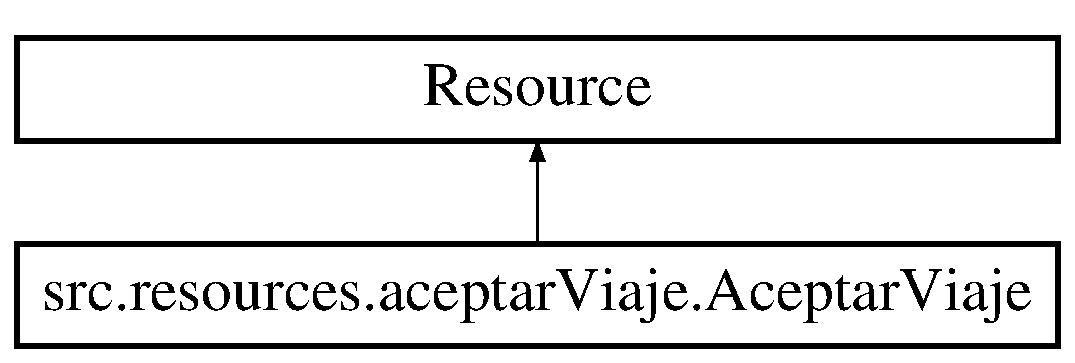
\includegraphics[height=2.000000cm]{classsrc_1_1resources_1_1aceptar_viaje_1_1_aceptar_viaje}
\end{center}
\end{figure}
\subsection*{Métodos públicos}
\begin{DoxyCompactItemize}
\item 
\hypertarget{classsrc_1_1resources_1_1aceptar_viaje_1_1_aceptar_viaje_aa0409475ce903baca3b2aefbb48d0e61}{def {\bfseries \-\_\-\-\_\-init\-\_\-\-\_\-}}\label{classsrc_1_1resources_1_1aceptar_viaje_1_1_aceptar_viaje_aa0409475ce903baca3b2aefbb48d0e61}

\item 
def \hyperlink{classsrc_1_1resources_1_1aceptar_viaje_1_1_aceptar_viaje_a83eb87e969accc14f808c6af720f75e1}{post}
\begin{DoxyCompactList}\small\item\em Acepta un viaje y borra todos los otros. \end{DoxyCompactList}\item 
def \hyperlink{classsrc_1_1resources_1_1aceptar_viaje_1_1_aceptar_viaje_a03e5a5b1e3010f3dcdbe9e9af815c0d4}{dar\-\_\-alta}
\begin{DoxyCompactList}\small\item\em Da de alta el viaje en el Shared Server. \end{DoxyCompactList}\end{DoxyCompactItemize}
\subsection*{Atributos públicos}
\begin{DoxyCompactItemize}
\item 
\hypertarget{classsrc_1_1resources_1_1aceptar_viaje_1_1_aceptar_viaje_affd7a9ee72935b1e44374caee1a5548d}{{\bfseries autenticador}}\label{classsrc_1_1resources_1_1aceptar_viaje_1_1_aceptar_viaje_affd7a9ee72935b1e44374caee1a5548d}

\end{DoxyCompactItemize}
\subsection*{Métodos privados}
\begin{DoxyCompactItemize}
\item 
def \hyperlink{classsrc_1_1resources_1_1aceptar_viaje_1_1_aceptar_viaje_a4bd84587a95e42ae2a42d7d4066a5d6e}{\-\_\-validar\-\_\-token}
\begin{DoxyCompactList}\small\item\em Valida al usuario. \end{DoxyCompactList}\item 
def \hyperlink{classsrc_1_1resources_1_1aceptar_viaje_1_1_aceptar_viaje_a2ad5306a2503932d0ae230665e6681a9}{\-\_\-aceptar\-\_\-viaje}
\begin{DoxyCompactList}\small\item\em Acepta un viaje. \end{DoxyCompactList}\end{DoxyCompactItemize}


\subsection{Descripción detallada}
Clase para aceptar un viaje de un chofer. 



\subsection{Documentación de las funciones miembro}
\hypertarget{classsrc_1_1resources_1_1aceptar_viaje_1_1_aceptar_viaje_a2ad5306a2503932d0ae230665e6681a9}{\index{src\-::resources\-::aceptar\-Viaje\-::\-Aceptar\-Viaje@{src\-::resources\-::aceptar\-Viaje\-::\-Aceptar\-Viaje}!\-\_\-aceptar\-\_\-viaje@{\-\_\-aceptar\-\_\-viaje}}
\index{\-\_\-aceptar\-\_\-viaje@{\-\_\-aceptar\-\_\-viaje}!src::resources::aceptarViaje::AceptarViaje@{src\-::resources\-::aceptar\-Viaje\-::\-Aceptar\-Viaje}}
\subsubsection[{\-\_\-aceptar\-\_\-viaje}]{\setlength{\rightskip}{0pt plus 5cm}def src.\-resources.\-aceptar\-Viaje.\-Aceptar\-Viaje.\-\_\-aceptar\-\_\-viaje (
\begin{DoxyParamCaption}
\item[{}]{self, }
\item[{}]{I\-D\-Usuario, }
\item[{}]{I\-D\-Viaje}
\end{DoxyParamCaption}
)\hspace{0.3cm}{\ttfamily [private]}}}\label{classsrc_1_1resources_1_1aceptar_viaje_1_1_aceptar_viaje_a2ad5306a2503932d0ae230665e6681a9}


Acepta un viaje. 

\hypertarget{classsrc_1_1resources_1_1aceptar_viaje_1_1_aceptar_viaje_a4bd84587a95e42ae2a42d7d4066a5d6e}{\index{src\-::resources\-::aceptar\-Viaje\-::\-Aceptar\-Viaje@{src\-::resources\-::aceptar\-Viaje\-::\-Aceptar\-Viaje}!\-\_\-validar\-\_\-token@{\-\_\-validar\-\_\-token}}
\index{\-\_\-validar\-\_\-token@{\-\_\-validar\-\_\-token}!src::resources::aceptarViaje::AceptarViaje@{src\-::resources\-::aceptar\-Viaje\-::\-Aceptar\-Viaje}}
\subsubsection[{\-\_\-validar\-\_\-token}]{\setlength{\rightskip}{0pt plus 5cm}def src.\-resources.\-aceptar\-Viaje.\-Aceptar\-Viaje.\-\_\-validar\-\_\-token (
\begin{DoxyParamCaption}
\item[{}]{self}
\end{DoxyParamCaption}
)\hspace{0.3cm}{\ttfamily [private]}}}\label{classsrc_1_1resources_1_1aceptar_viaje_1_1_aceptar_viaje_a4bd84587a95e42ae2a42d7d4066a5d6e}


Valida al usuario. 

\hypertarget{classsrc_1_1resources_1_1aceptar_viaje_1_1_aceptar_viaje_a03e5a5b1e3010f3dcdbe9e9af815c0d4}{\index{src\-::resources\-::aceptar\-Viaje\-::\-Aceptar\-Viaje@{src\-::resources\-::aceptar\-Viaje\-::\-Aceptar\-Viaje}!dar\-\_\-alta@{dar\-\_\-alta}}
\index{dar\-\_\-alta@{dar\-\_\-alta}!src::resources::aceptarViaje::AceptarViaje@{src\-::resources\-::aceptar\-Viaje\-::\-Aceptar\-Viaje}}
\subsubsection[{dar\-\_\-alta}]{\setlength{\rightskip}{0pt plus 5cm}def src.\-resources.\-aceptar\-Viaje.\-Aceptar\-Viaje.\-dar\-\_\-alta (
\begin{DoxyParamCaption}
\item[{}]{self, }
\item[{}]{viaje, }
\item[{}]{I\-D\-Usuario}
\end{DoxyParamCaption}
)}}\label{classsrc_1_1resources_1_1aceptar_viaje_1_1_aceptar_viaje_a03e5a5b1e3010f3dcdbe9e9af815c0d4}


Da de alta el viaje en el Shared Server. 

\hypertarget{classsrc_1_1resources_1_1aceptar_viaje_1_1_aceptar_viaje_a83eb87e969accc14f808c6af720f75e1}{\index{src\-::resources\-::aceptar\-Viaje\-::\-Aceptar\-Viaje@{src\-::resources\-::aceptar\-Viaje\-::\-Aceptar\-Viaje}!post@{post}}
\index{post@{post}!src::resources::aceptarViaje::AceptarViaje@{src\-::resources\-::aceptar\-Viaje\-::\-Aceptar\-Viaje}}
\subsubsection[{post}]{\setlength{\rightskip}{0pt plus 5cm}def src.\-resources.\-aceptar\-Viaje.\-Aceptar\-Viaje.\-post (
\begin{DoxyParamCaption}
\item[{}]{self, }
\item[{}]{I\-D\-Usuario, }
\item[{}]{I\-D\-Viaje}
\end{DoxyParamCaption}
)}}\label{classsrc_1_1resources_1_1aceptar_viaje_1_1_aceptar_viaje_a83eb87e969accc14f808c6af720f75e1}


Acepta un viaje y borra todos los otros. 



La documentación para esta clase fue generada a partir del siguiente fichero\-:\begin{DoxyCompactItemize}
\item 
src/resources/aceptar\-Viaje.\-py\end{DoxyCompactItemize}

\hypertarget{classsrc_1_1resources_1_1agregar_auto_usuario_1_1_agregar_auto_usuario}{\section{Referencia de la Clase src.\-resources.\-agregar\-Auto\-Usuario.\-Agregar\-Auto\-Usuario}
\label{classsrc_1_1resources_1_1agregar_auto_usuario_1_1_agregar_auto_usuario}\index{src.\-resources.\-agregar\-Auto\-Usuario.\-Agregar\-Auto\-Usuario@{src.\-resources.\-agregar\-Auto\-Usuario.\-Agregar\-Auto\-Usuario}}
}


Clase para agregar un auto a un usuario.  


Diagrama de herencias de src.\-resources.\-agregar\-Auto\-Usuario.\-Agregar\-Auto\-Usuario\begin{figure}[H]
\begin{center}
\leavevmode
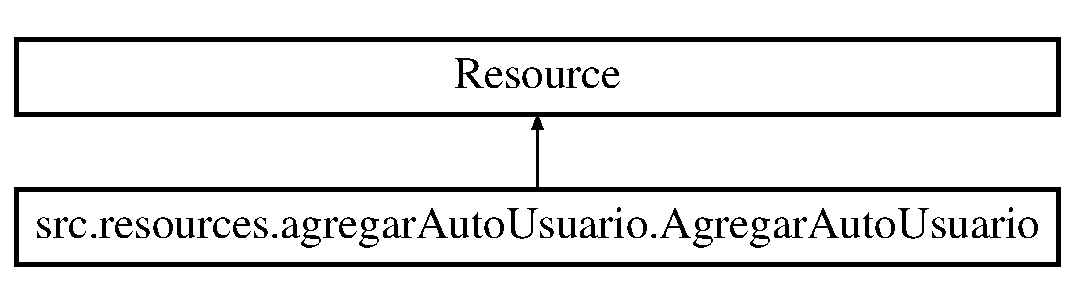
\includegraphics[height=2.000000cm]{classsrc_1_1resources_1_1agregar_auto_usuario_1_1_agregar_auto_usuario}
\end{center}
\end{figure}
\subsection*{Métodos públicos}
\begin{DoxyCompactItemize}
\item 
\hypertarget{classsrc_1_1resources_1_1agregar_auto_usuario_1_1_agregar_auto_usuario_ac497db4fdc43f3f587b2941704c1f3fd}{def {\bfseries \-\_\-\-\_\-init\-\_\-\-\_\-}}\label{classsrc_1_1resources_1_1agregar_auto_usuario_1_1_agregar_auto_usuario_ac497db4fdc43f3f587b2941704c1f3fd}

\item 
def \hyperlink{classsrc_1_1resources_1_1agregar_auto_usuario_1_1_agregar_auto_usuario_a2ac8095f1edcdd585d80155ddcc12344}{post}
\begin{DoxyCompactList}\small\item\em Asocia informacion de un nuevo auto a un usuario. \end{DoxyCompactList}\end{DoxyCompactItemize}
\subsection*{Atributos públicos}
\begin{DoxyCompactItemize}
\item 
\hypertarget{classsrc_1_1resources_1_1agregar_auto_usuario_1_1_agregar_auto_usuario_a815aacfb360ed387409ab7403e8bc8eb}{{\bfseries autenticador}}\label{classsrc_1_1resources_1_1agregar_auto_usuario_1_1_agregar_auto_usuario_a815aacfb360ed387409ab7403e8bc8eb}

\end{DoxyCompactItemize}
\subsection*{Métodos privados}
\begin{DoxyCompactItemize}
\item 
def \hyperlink{classsrc_1_1resources_1_1agregar_auto_usuario_1_1_agregar_auto_usuario_aef3d46a2434c1b8529ec3ff213d67b90}{\-\_\-get\-\_\-data\-\_\-from\-\_\-request}
\begin{DoxyCompactList}\small\item\em Obtiene la propiedad del json contenido de la request. \end{DoxyCompactList}\item 
def \hyperlink{classsrc_1_1resources_1_1agregar_auto_usuario_1_1_agregar_auto_usuario_ab5ea45024086cb5f15f0202f2289222c}{\-\_\-validate\-\_\-request}
\begin{DoxyCompactList}\small\item\em Valida que haya una request completa (se fija solo algun parametro). \end{DoxyCompactList}\item 
def \hyperlink{classsrc_1_1resources_1_1agregar_auto_usuario_1_1_agregar_auto_usuario_aac280b9aeeb811c61fb93540f253c7fa}{\-\_\-validar\-\_\-token}
\begin{DoxyCompactList}\small\item\em Valida al usuario. \end{DoxyCompactList}\item 
\hypertarget{classsrc_1_1resources_1_1agregar_auto_usuario_1_1_agregar_auto_usuario_a3d9a48144164751815316052e34bfdc0}{def {\bfseries \-\_\-obtener\-J\-S\-O\-N\-Propiedades\-Auto}}\label{classsrc_1_1resources_1_1agregar_auto_usuario_1_1_agregar_auto_usuario_a3d9a48144164751815316052e34bfdc0}

\end{DoxyCompactItemize}


\subsection{Descripción detallada}
Clase para agregar un auto a un usuario. 



\subsection{Documentación de las funciones miembro}
\hypertarget{classsrc_1_1resources_1_1agregar_auto_usuario_1_1_agregar_auto_usuario_aef3d46a2434c1b8529ec3ff213d67b90}{\index{src\-::resources\-::agregar\-Auto\-Usuario\-::\-Agregar\-Auto\-Usuario@{src\-::resources\-::agregar\-Auto\-Usuario\-::\-Agregar\-Auto\-Usuario}!\-\_\-get\-\_\-data\-\_\-from\-\_\-request@{\-\_\-get\-\_\-data\-\_\-from\-\_\-request}}
\index{\-\_\-get\-\_\-data\-\_\-from\-\_\-request@{\-\_\-get\-\_\-data\-\_\-from\-\_\-request}!src::resources::agregarAutoUsuario::AgregarAutoUsuario@{src\-::resources\-::agregar\-Auto\-Usuario\-::\-Agregar\-Auto\-Usuario}}
\subsubsection[{\-\_\-get\-\_\-data\-\_\-from\-\_\-request}]{\setlength{\rightskip}{0pt plus 5cm}def src.\-resources.\-agregar\-Auto\-Usuario.\-Agregar\-Auto\-Usuario.\-\_\-get\-\_\-data\-\_\-from\-\_\-request (
\begin{DoxyParamCaption}
\item[{}]{self, }
\item[{}]{nombre\-Propiedad, }
\item[{}]{defecto = {\ttfamily False}}
\end{DoxyParamCaption}
)\hspace{0.3cm}{\ttfamily [private]}}}\label{classsrc_1_1resources_1_1agregar_auto_usuario_1_1_agregar_auto_usuario_aef3d46a2434c1b8529ec3ff213d67b90}


Obtiene la propiedad del json contenido de la request. 

\hypertarget{classsrc_1_1resources_1_1agregar_auto_usuario_1_1_agregar_auto_usuario_aac280b9aeeb811c61fb93540f253c7fa}{\index{src\-::resources\-::agregar\-Auto\-Usuario\-::\-Agregar\-Auto\-Usuario@{src\-::resources\-::agregar\-Auto\-Usuario\-::\-Agregar\-Auto\-Usuario}!\-\_\-validar\-\_\-token@{\-\_\-validar\-\_\-token}}
\index{\-\_\-validar\-\_\-token@{\-\_\-validar\-\_\-token}!src::resources::agregarAutoUsuario::AgregarAutoUsuario@{src\-::resources\-::agregar\-Auto\-Usuario\-::\-Agregar\-Auto\-Usuario}}
\subsubsection[{\-\_\-validar\-\_\-token}]{\setlength{\rightskip}{0pt plus 5cm}def src.\-resources.\-agregar\-Auto\-Usuario.\-Agregar\-Auto\-Usuario.\-\_\-validar\-\_\-token (
\begin{DoxyParamCaption}
\item[{}]{self}
\end{DoxyParamCaption}
)\hspace{0.3cm}{\ttfamily [private]}}}\label{classsrc_1_1resources_1_1agregar_auto_usuario_1_1_agregar_auto_usuario_aac280b9aeeb811c61fb93540f253c7fa}


Valida al usuario. 

\hypertarget{classsrc_1_1resources_1_1agregar_auto_usuario_1_1_agregar_auto_usuario_ab5ea45024086cb5f15f0202f2289222c}{\index{src\-::resources\-::agregar\-Auto\-Usuario\-::\-Agregar\-Auto\-Usuario@{src\-::resources\-::agregar\-Auto\-Usuario\-::\-Agregar\-Auto\-Usuario}!\-\_\-validate\-\_\-request@{\-\_\-validate\-\_\-request}}
\index{\-\_\-validate\-\_\-request@{\-\_\-validate\-\_\-request}!src::resources::agregarAutoUsuario::AgregarAutoUsuario@{src\-::resources\-::agregar\-Auto\-Usuario\-::\-Agregar\-Auto\-Usuario}}
\subsubsection[{\-\_\-validate\-\_\-request}]{\setlength{\rightskip}{0pt plus 5cm}def src.\-resources.\-agregar\-Auto\-Usuario.\-Agregar\-Auto\-Usuario.\-\_\-validate\-\_\-request (
\begin{DoxyParamCaption}
\item[{}]{self}
\end{DoxyParamCaption}
)\hspace{0.3cm}{\ttfamily [private]}}}\label{classsrc_1_1resources_1_1agregar_auto_usuario_1_1_agregar_auto_usuario_ab5ea45024086cb5f15f0202f2289222c}


Valida que haya una request completa (se fija solo algun parametro). 

\hypertarget{classsrc_1_1resources_1_1agregar_auto_usuario_1_1_agregar_auto_usuario_a2ac8095f1edcdd585d80155ddcc12344}{\index{src\-::resources\-::agregar\-Auto\-Usuario\-::\-Agregar\-Auto\-Usuario@{src\-::resources\-::agregar\-Auto\-Usuario\-::\-Agregar\-Auto\-Usuario}!post@{post}}
\index{post@{post}!src::resources::agregarAutoUsuario::AgregarAutoUsuario@{src\-::resources\-::agregar\-Auto\-Usuario\-::\-Agregar\-Auto\-Usuario}}
\subsubsection[{post}]{\setlength{\rightskip}{0pt plus 5cm}def src.\-resources.\-agregar\-Auto\-Usuario.\-Agregar\-Auto\-Usuario.\-post (
\begin{DoxyParamCaption}
\item[{}]{self, }
\item[{}]{I\-D\-Usuario}
\end{DoxyParamCaption}
)}}\label{classsrc_1_1resources_1_1agregar_auto_usuario_1_1_agregar_auto_usuario_a2ac8095f1edcdd585d80155ddcc12344}


Asocia informacion de un nuevo auto a un usuario. 



La documentación para esta clase fue generada a partir del siguiente fichero\-:\begin{DoxyCompactItemize}
\item 
src/resources/agregar\-Auto\-Usuario.\-py\end{DoxyCompactItemize}

\hypertarget{classsrc_1_1resources_1_1agregar_posible_viaje_1_1_agregar_posible_viaje}{\section{Referencia de la Clase src.\-resources.\-agregar\-Posible\-Viaje.\-Agregar\-Posible\-Viaje}
\label{classsrc_1_1resources_1_1agregar_posible_viaje_1_1_agregar_posible_viaje}\index{src.\-resources.\-agregar\-Posible\-Viaje.\-Agregar\-Posible\-Viaje@{src.\-resources.\-agregar\-Posible\-Viaje.\-Agregar\-Posible\-Viaje}}
}


Clase para agregar un viaje a la lista de posibles viajes de un chofer.  


Diagrama de herencias de src.\-resources.\-agregar\-Posible\-Viaje.\-Agregar\-Posible\-Viaje\begin{figure}[H]
\begin{center}
\leavevmode
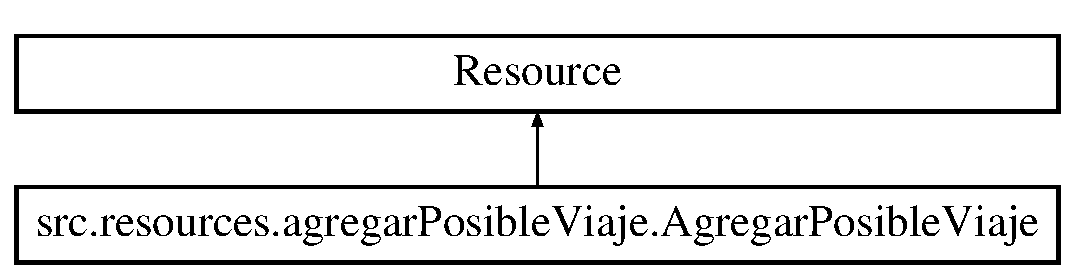
\includegraphics[height=2.000000cm]{classsrc_1_1resources_1_1agregar_posible_viaje_1_1_agregar_posible_viaje}
\end{center}
\end{figure}
\subsection*{Métodos públicos}
\begin{DoxyCompactItemize}
\item 
\hypertarget{classsrc_1_1resources_1_1agregar_posible_viaje_1_1_agregar_posible_viaje_a0eb8e6dc028544d8ab763ad50e18b734}{def {\bfseries \-\_\-\-\_\-init\-\_\-\-\_\-}}\label{classsrc_1_1resources_1_1agregar_posible_viaje_1_1_agregar_posible_viaje_a0eb8e6dc028544d8ab763ad50e18b734}

\item 
def \hyperlink{classsrc_1_1resources_1_1agregar_posible_viaje_1_1_agregar_posible_viaje_a6842769a8d9d3ba65137ea0b9bd0d21c}{post}
\begin{DoxyCompactList}\small\item\em Agrega la informacion del viaje posible. \end{DoxyCompactList}\end{DoxyCompactItemize}
\subsection*{Atributos públicos}
\begin{DoxyCompactItemize}
\item 
\hypertarget{classsrc_1_1resources_1_1agregar_posible_viaje_1_1_agregar_posible_viaje_a044f943b782b424b5f09168599465953}{{\bfseries U\-R\-L\-Directions}}\label{classsrc_1_1resources_1_1agregar_posible_viaje_1_1_agregar_posible_viaje_a044f943b782b424b5f09168599465953}

\item 
\hypertarget{classsrc_1_1resources_1_1agregar_posible_viaje_1_1_agregar_posible_viaje_a0f9fde264ccc7f4c1e2734827907f95d}{{\bfseries U\-R\-L}}\label{classsrc_1_1resources_1_1agregar_posible_viaje_1_1_agregar_posible_viaje_a0f9fde264ccc7f4c1e2734827907f95d}

\item 
\hypertarget{classsrc_1_1resources_1_1agregar_posible_viaje_1_1_agregar_posible_viaje_a590d83ac0d66e6fa577de0a2b333486d}{{\bfseries autenticador}}\label{classsrc_1_1resources_1_1agregar_posible_viaje_1_1_agregar_posible_viaje_a590d83ac0d66e6fa577de0a2b333486d}

\item 
\hypertarget{classsrc_1_1resources_1_1agregar_posible_viaje_1_1_agregar_posible_viaje_a582f351bc5720271aac35ab4944c685f}{{\bfseries conectividad}}\label{classsrc_1_1resources_1_1agregar_posible_viaje_1_1_agregar_posible_viaje_a582f351bc5720271aac35ab4944c685f}

\item 
\hypertarget{classsrc_1_1resources_1_1agregar_posible_viaje_1_1_agregar_posible_viaje_ae388d6c98caf2992ad496091015ff7ee}{{\bfseries I\-D\-Usuario}}\label{classsrc_1_1resources_1_1agregar_posible_viaje_1_1_agregar_posible_viaje_ae388d6c98caf2992ad496091015ff7ee}

\end{DoxyCompactItemize}
\subsection*{Métodos privados}
\begin{DoxyCompactItemize}
\item 
def \hyperlink{classsrc_1_1resources_1_1agregar_posible_viaje_1_1_agregar_posible_viaje_a5e1895bbbd0a99c308c8e64ab31d849d}{\-\_\-get\-\_\-data\-\_\-from\-\_\-request}
\begin{DoxyCompactList}\small\item\em Obtiene la propiedad del json contenido de la request. \end{DoxyCompactList}\item 
def \hyperlink{classsrc_1_1resources_1_1agregar_posible_viaje_1_1_agregar_posible_viaje_a07ca4d8c5ea2ab8f8c9b15ef780b2e51}{\-\_\-validate\-\_\-request}
\begin{DoxyCompactList}\small\item\em Valida que haya una request completa. \end{DoxyCompactList}\item 
def \hyperlink{classsrc_1_1resources_1_1agregar_posible_viaje_1_1_agregar_posible_viaje_a2d8499cb043b289c3bd8ff3e8cdb2c7e}{\-\_\-validar\-\_\-token}
\begin{DoxyCompactList}\small\item\em Valida al usuario. \end{DoxyCompactList}\item 
def \hyperlink{classsrc_1_1resources_1_1agregar_posible_viaje_1_1_agregar_posible_viaje_a9fe9e1a9fe96f5c88beb0cf5dc0df429}{\-\_\-obtener\-\_\-costo\-\_\-viaje}
\begin{DoxyCompactList}\small\item\em le pide al shared server la cotizacion del viaje. \end{DoxyCompactList}\item 
def \hyperlink{classsrc_1_1resources_1_1agregar_posible_viaje_1_1_agregar_posible_viaje_af122e9531612ea88ecf6fadc18805fca}{\-\_\-obtener\-J\-S\-O\-N\-Viaje}
\begin{DoxyCompactList}\small\item\em Obtiene toda la informacion y crea el J\-S\-O\-N de datos del viaje. \end{DoxyCompactList}\item 
def \hyperlink{classsrc_1_1resources_1_1agregar_posible_viaje_1_1_agregar_posible_viaje_a3da09dd6130bae191361f3224a39c64d}{\-\_\-obtener\-\_\-\-I\-D\-\_\-viaje}
\begin{DoxyCompactList}\small\item\em Obtiene el id del viaje a insertar usando el contador autoincremental de cada conductor. \end{DoxyCompactList}\item 
def \hyperlink{classsrc_1_1resources_1_1agregar_posible_viaje_1_1_agregar_posible_viaje_a58a02362fca47d96278e36be3dd42ad7}{\-\_\-acondicionar\-J\-S\-O\-N\-Usuario}
\begin{DoxyCompactList}\small\item\em Metodo intermedio para asegurar la normalizacion de la informacion. \end{DoxyCompactList}\item 
\hypertarget{classsrc_1_1resources_1_1agregar_posible_viaje_1_1_agregar_posible_viaje_ad04b5932af3f4ae57f3a49c881c6530c}{def {\bfseries \-\_\-guardar\-\_\-viaje\-\_\-mongo}}\label{classsrc_1_1resources_1_1agregar_posible_viaje_1_1_agregar_posible_viaje_ad04b5932af3f4ae57f3a49c881c6530c}

\item 
def \hyperlink{classsrc_1_1resources_1_1agregar_posible_viaje_1_1_agregar_posible_viaje_a1526401fbb0f58fb43d607d2e686ef31}{\-\_\-acondicionar\-J\-S\-O\-N\-Ruta}
\begin{DoxyCompactList}\small\item\em Acondiciona la salida de Google Directions. \end{DoxyCompactList}\item 
def \hyperlink{classsrc_1_1resources_1_1agregar_posible_viaje_1_1_agregar_posible_viaje_a42f28fac7e1c6df7705f6d9298d19704}{\-\_\-obtener\-\_\-ruta\-\_\-directions}
\begin{DoxyCompactList}\small\item\em Realiza la peticion a Google Directions. \end{DoxyCompactList}\item 
def \hyperlink{classsrc_1_1resources_1_1agregar_posible_viaje_1_1_agregar_posible_viaje_ae4dbe06fe2e8c504ecc8d86275881aa3}{\-\_\-calcular\-\_\-ruta}
\begin{DoxyCompactList}\small\item\em Pide el servicio a Google Directions. \end{DoxyCompactList}\end{DoxyCompactItemize}


\subsection{Descripción detallada}
Clase para agregar un viaje a la lista de posibles viajes de un chofer. 



\subsection{Documentación de las funciones miembro}
\hypertarget{classsrc_1_1resources_1_1agregar_posible_viaje_1_1_agregar_posible_viaje_a1526401fbb0f58fb43d607d2e686ef31}{\index{src\-::resources\-::agregar\-Posible\-Viaje\-::\-Agregar\-Posible\-Viaje@{src\-::resources\-::agregar\-Posible\-Viaje\-::\-Agregar\-Posible\-Viaje}!\-\_\-acondicionar\-J\-S\-O\-N\-Ruta@{\-\_\-acondicionar\-J\-S\-O\-N\-Ruta}}
\index{\-\_\-acondicionar\-J\-S\-O\-N\-Ruta@{\-\_\-acondicionar\-J\-S\-O\-N\-Ruta}!src::resources::agregarPosibleViaje::AgregarPosibleViaje@{src\-::resources\-::agregar\-Posible\-Viaje\-::\-Agregar\-Posible\-Viaje}}
\subsubsection[{\-\_\-acondicionar\-J\-S\-O\-N\-Ruta}]{\setlength{\rightskip}{0pt plus 5cm}def src.\-resources.\-agregar\-Posible\-Viaje.\-Agregar\-Posible\-Viaje.\-\_\-acondicionar\-J\-S\-O\-N\-Ruta (
\begin{DoxyParamCaption}
\item[{}]{self, }
\item[{}]{datos}
\end{DoxyParamCaption}
)\hspace{0.3cm}{\ttfamily [private]}}}\label{classsrc_1_1resources_1_1agregar_posible_viaje_1_1_agregar_posible_viaje_a1526401fbb0f58fb43d607d2e686ef31}


Acondiciona la salida de Google Directions. 


\begin{DoxyParams}{Parámetros}
{\em datos} & Es lo que devuelva Google Directions. \\
\hline
\end{DoxyParams}
\hypertarget{classsrc_1_1resources_1_1agregar_posible_viaje_1_1_agregar_posible_viaje_a58a02362fca47d96278e36be3dd42ad7}{\index{src\-::resources\-::agregar\-Posible\-Viaje\-::\-Agregar\-Posible\-Viaje@{src\-::resources\-::agregar\-Posible\-Viaje\-::\-Agregar\-Posible\-Viaje}!\-\_\-acondicionar\-J\-S\-O\-N\-Usuario@{\-\_\-acondicionar\-J\-S\-O\-N\-Usuario}}
\index{\-\_\-acondicionar\-J\-S\-O\-N\-Usuario@{\-\_\-acondicionar\-J\-S\-O\-N\-Usuario}!src::resources::agregarPosibleViaje::AgregarPosibleViaje@{src\-::resources\-::agregar\-Posible\-Viaje\-::\-Agregar\-Posible\-Viaje}}
\subsubsection[{\-\_\-acondicionar\-J\-S\-O\-N\-Usuario}]{\setlength{\rightskip}{0pt plus 5cm}def src.\-resources.\-agregar\-Posible\-Viaje.\-Agregar\-Posible\-Viaje.\-\_\-acondicionar\-J\-S\-O\-N\-Usuario (
\begin{DoxyParamCaption}
\item[{}]{self, }
\item[{}]{datos}
\end{DoxyParamCaption}
)\hspace{0.3cm}{\ttfamily [private]}}}\label{classsrc_1_1resources_1_1agregar_posible_viaje_1_1_agregar_posible_viaje_a58a02362fca47d96278e36be3dd42ad7}


Metodo intermedio para asegurar la normalizacion de la informacion. 

\hypertarget{classsrc_1_1resources_1_1agregar_posible_viaje_1_1_agregar_posible_viaje_ae4dbe06fe2e8c504ecc8d86275881aa3}{\index{src\-::resources\-::agregar\-Posible\-Viaje\-::\-Agregar\-Posible\-Viaje@{src\-::resources\-::agregar\-Posible\-Viaje\-::\-Agregar\-Posible\-Viaje}!\-\_\-calcular\-\_\-ruta@{\-\_\-calcular\-\_\-ruta}}
\index{\-\_\-calcular\-\_\-ruta@{\-\_\-calcular\-\_\-ruta}!src::resources::agregarPosibleViaje::AgregarPosibleViaje@{src\-::resources\-::agregar\-Posible\-Viaje\-::\-Agregar\-Posible\-Viaje}}
\subsubsection[{\-\_\-calcular\-\_\-ruta}]{\setlength{\rightskip}{0pt plus 5cm}def src.\-resources.\-agregar\-Posible\-Viaje.\-Agregar\-Posible\-Viaje.\-\_\-calcular\-\_\-ruta (
\begin{DoxyParamCaption}
\item[{}]{self, }
\item[{}]{origen, }
\item[{}]{destino}
\end{DoxyParamCaption}
)\hspace{0.3cm}{\ttfamily [private]}}}\label{classsrc_1_1resources_1_1agregar_posible_viaje_1_1_agregar_posible_viaje_ae4dbe06fe2e8c504ecc8d86275881aa3}


Pide el servicio a Google Directions. 

\hypertarget{classsrc_1_1resources_1_1agregar_posible_viaje_1_1_agregar_posible_viaje_a5e1895bbbd0a99c308c8e64ab31d849d}{\index{src\-::resources\-::agregar\-Posible\-Viaje\-::\-Agregar\-Posible\-Viaje@{src\-::resources\-::agregar\-Posible\-Viaje\-::\-Agregar\-Posible\-Viaje}!\-\_\-get\-\_\-data\-\_\-from\-\_\-request@{\-\_\-get\-\_\-data\-\_\-from\-\_\-request}}
\index{\-\_\-get\-\_\-data\-\_\-from\-\_\-request@{\-\_\-get\-\_\-data\-\_\-from\-\_\-request}!src::resources::agregarPosibleViaje::AgregarPosibleViaje@{src\-::resources\-::agregar\-Posible\-Viaje\-::\-Agregar\-Posible\-Viaje}}
\subsubsection[{\-\_\-get\-\_\-data\-\_\-from\-\_\-request}]{\setlength{\rightskip}{0pt plus 5cm}def src.\-resources.\-agregar\-Posible\-Viaje.\-Agregar\-Posible\-Viaje.\-\_\-get\-\_\-data\-\_\-from\-\_\-request (
\begin{DoxyParamCaption}
\item[{}]{self, }
\item[{}]{nombre\-Propiedad}
\end{DoxyParamCaption}
)\hspace{0.3cm}{\ttfamily [private]}}}\label{classsrc_1_1resources_1_1agregar_posible_viaje_1_1_agregar_posible_viaje_a5e1895bbbd0a99c308c8e64ab31d849d}


Obtiene la propiedad del json contenido de la request. 

\hypertarget{classsrc_1_1resources_1_1agregar_posible_viaje_1_1_agregar_posible_viaje_a9fe9e1a9fe96f5c88beb0cf5dc0df429}{\index{src\-::resources\-::agregar\-Posible\-Viaje\-::\-Agregar\-Posible\-Viaje@{src\-::resources\-::agregar\-Posible\-Viaje\-::\-Agregar\-Posible\-Viaje}!\-\_\-obtener\-\_\-costo\-\_\-viaje@{\-\_\-obtener\-\_\-costo\-\_\-viaje}}
\index{\-\_\-obtener\-\_\-costo\-\_\-viaje@{\-\_\-obtener\-\_\-costo\-\_\-viaje}!src::resources::agregarPosibleViaje::AgregarPosibleViaje@{src\-::resources\-::agregar\-Posible\-Viaje\-::\-Agregar\-Posible\-Viaje}}
\subsubsection[{\-\_\-obtener\-\_\-costo\-\_\-viaje}]{\setlength{\rightskip}{0pt plus 5cm}def src.\-resources.\-agregar\-Posible\-Viaje.\-Agregar\-Posible\-Viaje.\-\_\-obtener\-\_\-costo\-\_\-viaje (
\begin{DoxyParamCaption}
\item[{}]{self, }
\item[{}]{I\-D\-Usuario, }
\item[{}]{I\-D\-Pasajero, }
\item[{}]{ruta}
\end{DoxyParamCaption}
)\hspace{0.3cm}{\ttfamily [private]}}}\label{classsrc_1_1resources_1_1agregar_posible_viaje_1_1_agregar_posible_viaje_a9fe9e1a9fe96f5c88beb0cf5dc0df429}


le pide al shared server la cotizacion del viaje. 

\hypertarget{classsrc_1_1resources_1_1agregar_posible_viaje_1_1_agregar_posible_viaje_a3da09dd6130bae191361f3224a39c64d}{\index{src\-::resources\-::agregar\-Posible\-Viaje\-::\-Agregar\-Posible\-Viaje@{src\-::resources\-::agregar\-Posible\-Viaje\-::\-Agregar\-Posible\-Viaje}!\-\_\-obtener\-\_\-\-I\-D\-\_\-viaje@{\-\_\-obtener\-\_\-\-I\-D\-\_\-viaje}}
\index{\-\_\-obtener\-\_\-\-I\-D\-\_\-viaje@{\-\_\-obtener\-\_\-\-I\-D\-\_\-viaje}!src::resources::agregarPosibleViaje::AgregarPosibleViaje@{src\-::resources\-::agregar\-Posible\-Viaje\-::\-Agregar\-Posible\-Viaje}}
\subsubsection[{\-\_\-obtener\-\_\-\-I\-D\-\_\-viaje}]{\setlength{\rightskip}{0pt plus 5cm}def src.\-resources.\-agregar\-Posible\-Viaje.\-Agregar\-Posible\-Viaje.\-\_\-obtener\-\_\-\-I\-D\-\_\-viaje (
\begin{DoxyParamCaption}
\item[{}]{self, }
\item[{}]{I\-D\-Usuario}
\end{DoxyParamCaption}
)\hspace{0.3cm}{\ttfamily [private]}}}\label{classsrc_1_1resources_1_1agregar_posible_viaje_1_1_agregar_posible_viaje_a3da09dd6130bae191361f3224a39c64d}


Obtiene el id del viaje a insertar usando el contador autoincremental de cada conductor. 

\hypertarget{classsrc_1_1resources_1_1agregar_posible_viaje_1_1_agregar_posible_viaje_a42f28fac7e1c6df7705f6d9298d19704}{\index{src\-::resources\-::agregar\-Posible\-Viaje\-::\-Agregar\-Posible\-Viaje@{src\-::resources\-::agregar\-Posible\-Viaje\-::\-Agregar\-Posible\-Viaje}!\-\_\-obtener\-\_\-ruta\-\_\-directions@{\-\_\-obtener\-\_\-ruta\-\_\-directions}}
\index{\-\_\-obtener\-\_\-ruta\-\_\-directions@{\-\_\-obtener\-\_\-ruta\-\_\-directions}!src::resources::agregarPosibleViaje::AgregarPosibleViaje@{src\-::resources\-::agregar\-Posible\-Viaje\-::\-Agregar\-Posible\-Viaje}}
\subsubsection[{\-\_\-obtener\-\_\-ruta\-\_\-directions}]{\setlength{\rightskip}{0pt plus 5cm}def src.\-resources.\-agregar\-Posible\-Viaje.\-Agregar\-Posible\-Viaje.\-\_\-obtener\-\_\-ruta\-\_\-directions (
\begin{DoxyParamCaption}
\item[{}]{self, }
\item[{}]{origen, }
\item[{}]{destino}
\end{DoxyParamCaption}
)\hspace{0.3cm}{\ttfamily [private]}}}\label{classsrc_1_1resources_1_1agregar_posible_viaje_1_1_agregar_posible_viaje_a42f28fac7e1c6df7705f6d9298d19704}


Realiza la peticion a Google Directions. 

\hypertarget{classsrc_1_1resources_1_1agregar_posible_viaje_1_1_agregar_posible_viaje_af122e9531612ea88ecf6fadc18805fca}{\index{src\-::resources\-::agregar\-Posible\-Viaje\-::\-Agregar\-Posible\-Viaje@{src\-::resources\-::agregar\-Posible\-Viaje\-::\-Agregar\-Posible\-Viaje}!\-\_\-obtener\-J\-S\-O\-N\-Viaje@{\-\_\-obtener\-J\-S\-O\-N\-Viaje}}
\index{\-\_\-obtener\-J\-S\-O\-N\-Viaje@{\-\_\-obtener\-J\-S\-O\-N\-Viaje}!src::resources::agregarPosibleViaje::AgregarPosibleViaje@{src\-::resources\-::agregar\-Posible\-Viaje\-::\-Agregar\-Posible\-Viaje}}
\subsubsection[{\-\_\-obtener\-J\-S\-O\-N\-Viaje}]{\setlength{\rightskip}{0pt plus 5cm}def src.\-resources.\-agregar\-Posible\-Viaje.\-Agregar\-Posible\-Viaje.\-\_\-obtener\-J\-S\-O\-N\-Viaje (
\begin{DoxyParamCaption}
\item[{}]{self}
\end{DoxyParamCaption}
)\hspace{0.3cm}{\ttfamily [private]}}}\label{classsrc_1_1resources_1_1agregar_posible_viaje_1_1_agregar_posible_viaje_af122e9531612ea88ecf6fadc18805fca}


Obtiene toda la informacion y crea el J\-S\-O\-N de datos del viaje. 

\begin{DoxyVerb}Pide la informacion del usuario al Shared Server.\end{DoxyVerb}
 \hypertarget{classsrc_1_1resources_1_1agregar_posible_viaje_1_1_agregar_posible_viaje_a2d8499cb043b289c3bd8ff3e8cdb2c7e}{\index{src\-::resources\-::agregar\-Posible\-Viaje\-::\-Agregar\-Posible\-Viaje@{src\-::resources\-::agregar\-Posible\-Viaje\-::\-Agregar\-Posible\-Viaje}!\-\_\-validar\-\_\-token@{\-\_\-validar\-\_\-token}}
\index{\-\_\-validar\-\_\-token@{\-\_\-validar\-\_\-token}!src::resources::agregarPosibleViaje::AgregarPosibleViaje@{src\-::resources\-::agregar\-Posible\-Viaje\-::\-Agregar\-Posible\-Viaje}}
\subsubsection[{\-\_\-validar\-\_\-token}]{\setlength{\rightskip}{0pt plus 5cm}def src.\-resources.\-agregar\-Posible\-Viaje.\-Agregar\-Posible\-Viaje.\-\_\-validar\-\_\-token (
\begin{DoxyParamCaption}
\item[{}]{self}
\end{DoxyParamCaption}
)\hspace{0.3cm}{\ttfamily [private]}}}\label{classsrc_1_1resources_1_1agregar_posible_viaje_1_1_agregar_posible_viaje_a2d8499cb043b289c3bd8ff3e8cdb2c7e}


Valida al usuario. 

\hypertarget{classsrc_1_1resources_1_1agregar_posible_viaje_1_1_agregar_posible_viaje_a07ca4d8c5ea2ab8f8c9b15ef780b2e51}{\index{src\-::resources\-::agregar\-Posible\-Viaje\-::\-Agregar\-Posible\-Viaje@{src\-::resources\-::agregar\-Posible\-Viaje\-::\-Agregar\-Posible\-Viaje}!\-\_\-validate\-\_\-request@{\-\_\-validate\-\_\-request}}
\index{\-\_\-validate\-\_\-request@{\-\_\-validate\-\_\-request}!src::resources::agregarPosibleViaje::AgregarPosibleViaje@{src\-::resources\-::agregar\-Posible\-Viaje\-::\-Agregar\-Posible\-Viaje}}
\subsubsection[{\-\_\-validate\-\_\-request}]{\setlength{\rightskip}{0pt plus 5cm}def src.\-resources.\-agregar\-Posible\-Viaje.\-Agregar\-Posible\-Viaje.\-\_\-validate\-\_\-request (
\begin{DoxyParamCaption}
\item[{}]{self}
\end{DoxyParamCaption}
)\hspace{0.3cm}{\ttfamily [private]}}}\label{classsrc_1_1resources_1_1agregar_posible_viaje_1_1_agregar_posible_viaje_a07ca4d8c5ea2ab8f8c9b15ef780b2e51}


Valida que haya una request completa. 

\hypertarget{classsrc_1_1resources_1_1agregar_posible_viaje_1_1_agregar_posible_viaje_a6842769a8d9d3ba65137ea0b9bd0d21c}{\index{src\-::resources\-::agregar\-Posible\-Viaje\-::\-Agregar\-Posible\-Viaje@{src\-::resources\-::agregar\-Posible\-Viaje\-::\-Agregar\-Posible\-Viaje}!post@{post}}
\index{post@{post}!src::resources::agregarPosibleViaje::AgregarPosibleViaje@{src\-::resources\-::agregar\-Posible\-Viaje\-::\-Agregar\-Posible\-Viaje}}
\subsubsection[{post}]{\setlength{\rightskip}{0pt plus 5cm}def src.\-resources.\-agregar\-Posible\-Viaje.\-Agregar\-Posible\-Viaje.\-post (
\begin{DoxyParamCaption}
\item[{}]{self, }
\item[{}]{I\-D\-Usuario}
\end{DoxyParamCaption}
)}}\label{classsrc_1_1resources_1_1agregar_posible_viaje_1_1_agregar_posible_viaje_a6842769a8d9d3ba65137ea0b9bd0d21c}


Agrega la informacion del viaje posible. 



La documentación para esta clase fue generada a partir del siguiente fichero\-:\begin{DoxyCompactItemize}
\item 
src/resources/agregar\-Posible\-Viaje.\-py\end{DoxyCompactItemize}

\hypertarget{classsrc_1_1resources_1_1auth_1_1_auth}{\section{Referencia de la Clase src.\-resources.\-auth.\-Auth}
\label{classsrc_1_1resources_1_1auth_1_1_auth}\index{src.\-resources.\-auth.\-Auth@{src.\-resources.\-auth.\-Auth}}
}


Clase para autenticacion y creacion del Token.  


Diagrama de herencias de src.\-resources.\-auth.\-Auth\begin{figure}[H]
\begin{center}
\leavevmode
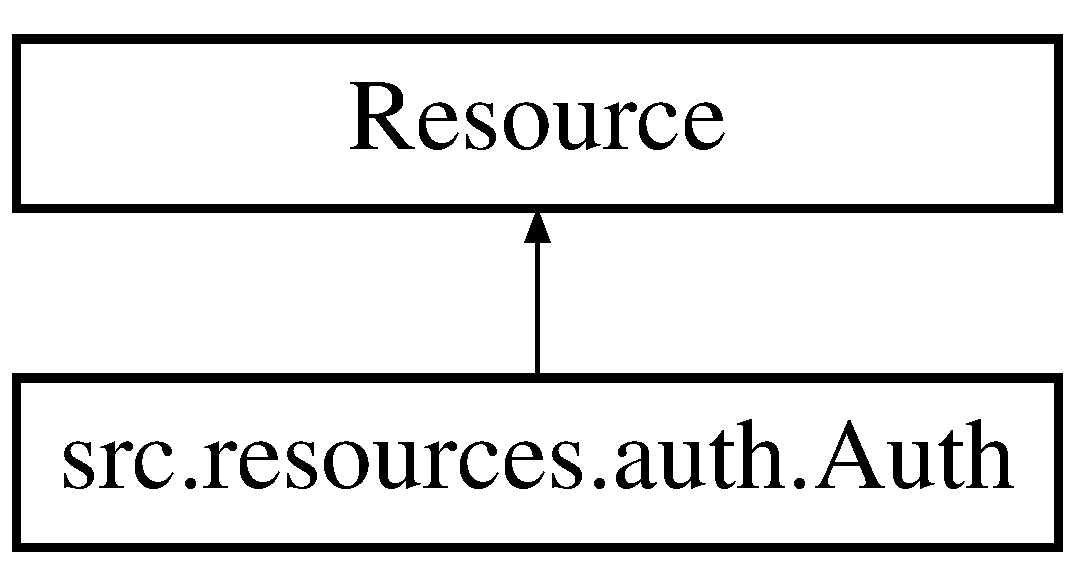
\includegraphics[height=2.000000cm]{classsrc_1_1resources_1_1auth_1_1_auth}
\end{center}
\end{figure}
\subsection*{Métodos públicos}
\begin{DoxyCompactItemize}
\item 
\hypertarget{classsrc_1_1resources_1_1auth_1_1_auth_a2d64661c266e0acecb9f982c74c255bf}{def {\bfseries \-\_\-\-\_\-init\-\_\-\-\_\-}}\label{classsrc_1_1resources_1_1auth_1_1_auth_a2d64661c266e0acecb9f982c74c255bf}

\item 
def \hyperlink{classsrc_1_1resources_1_1auth_1_1_auth_a1dc17d25fd4327120f782367cad81b39}{post}
\begin{DoxyCompactList}\small\item\em Autentica al usuario una unica vez. \end{DoxyCompactList}\end{DoxyCompactItemize}
\subsection*{Atributos públicos}
\begin{DoxyCompactItemize}
\item 
\hypertarget{classsrc_1_1resources_1_1auth_1_1_auth_ab31b5b7d3f7117c7030fb0bb13ec3d4e}{{\bfseries conectividad}}\label{classsrc_1_1resources_1_1auth_1_1_auth_ab31b5b7d3f7117c7030fb0bb13ec3d4e}

\item 
\hypertarget{classsrc_1_1resources_1_1auth_1_1_auth_a6f941c20282acda0048ff950c20b6020}{{\bfseries autenticador}}\label{classsrc_1_1resources_1_1auth_1_1_auth_a6f941c20282acda0048ff950c20b6020}

\item 
\hypertarget{classsrc_1_1resources_1_1auth_1_1_auth_a454d6c5e4da3b215b9067a01b4b653ea}{{\bfseries id}}\label{classsrc_1_1resources_1_1auth_1_1_auth_a454d6c5e4da3b215b9067a01b4b653ea}

\item 
\hypertarget{classsrc_1_1resources_1_1auth_1_1_auth_a494e703175798885c56a25e8a203bba9}{{\bfseries tipo}}\label{classsrc_1_1resources_1_1auth_1_1_auth_a494e703175798885c56a25e8a203bba9}

\end{DoxyCompactItemize}
\subsection*{Métodos privados}
\begin{DoxyCompactItemize}
\item 
def \hyperlink{classsrc_1_1resources_1_1auth_1_1_auth_ad45756ae9f2bf3840d6fe69fc305f86d}{\-\_\-get\-\_\-user\-\_\-from\-\_\-request}
\begin{DoxyCompactList}\small\item\em Obtiene el nombre de usuario de la request. \end{DoxyCompactList}\item 
def \hyperlink{classsrc_1_1resources_1_1auth_1_1_auth_a85f8056c2198f62284ada1f9f40a72f2}{\-\_\-get\-\_\-hash\-Password\-\_\-from\-\_\-request}
\begin{DoxyCompactList}\small\item\em Obtiene la contrasena de la request. \end{DoxyCompactList}\item 
def \hyperlink{classsrc_1_1resources_1_1auth_1_1_auth_acd72657f2bddc8a60a3103f418460d57}{\-\_\-validate\-\_\-request}
\begin{DoxyCompactList}\small\item\em Valida que haya una request. \end{DoxyCompactList}\item 
def \hyperlink{classsrc_1_1resources_1_1auth_1_1_auth_ab140f80e50617f4d4f4a58b40391710f}{\-\_\-existe\-\_\-usuario\-\_\-en\-\_\-shared\-Server}
\begin{DoxyCompactList}\small\item\em Valida al usuario con el shared server. \end{DoxyCompactList}\end{DoxyCompactItemize}


\subsection{Descripción detallada}
Clase para autenticacion y creacion del Token. 



\subsection{Documentación de las funciones miembro}
\hypertarget{classsrc_1_1resources_1_1auth_1_1_auth_ab140f80e50617f4d4f4a58b40391710f}{\index{src\-::resources\-::auth\-::\-Auth@{src\-::resources\-::auth\-::\-Auth}!\-\_\-existe\-\_\-usuario\-\_\-en\-\_\-shared\-Server@{\-\_\-existe\-\_\-usuario\-\_\-en\-\_\-shared\-Server}}
\index{\-\_\-existe\-\_\-usuario\-\_\-en\-\_\-shared\-Server@{\-\_\-existe\-\_\-usuario\-\_\-en\-\_\-shared\-Server}!src::resources::auth::Auth@{src\-::resources\-::auth\-::\-Auth}}
\subsubsection[{\-\_\-existe\-\_\-usuario\-\_\-en\-\_\-shared\-Server}]{\setlength{\rightskip}{0pt plus 5cm}def src.\-resources.\-auth.\-Auth.\-\_\-existe\-\_\-usuario\-\_\-en\-\_\-shared\-Server (
\begin{DoxyParamCaption}
\item[{}]{self, }
\item[{}]{nombre\-Usuario, }
\item[{}]{contrasena}
\end{DoxyParamCaption}
)\hspace{0.3cm}{\ttfamily [private]}}}\label{classsrc_1_1resources_1_1auth_1_1_auth_ab140f80e50617f4d4f4a58b40391710f}


Valida al usuario con el shared server. 

\hypertarget{classsrc_1_1resources_1_1auth_1_1_auth_a85f8056c2198f62284ada1f9f40a72f2}{\index{src\-::resources\-::auth\-::\-Auth@{src\-::resources\-::auth\-::\-Auth}!\-\_\-get\-\_\-hash\-Password\-\_\-from\-\_\-request@{\-\_\-get\-\_\-hash\-Password\-\_\-from\-\_\-request}}
\index{\-\_\-get\-\_\-hash\-Password\-\_\-from\-\_\-request@{\-\_\-get\-\_\-hash\-Password\-\_\-from\-\_\-request}!src::resources::auth::Auth@{src\-::resources\-::auth\-::\-Auth}}
\subsubsection[{\-\_\-get\-\_\-hash\-Password\-\_\-from\-\_\-request}]{\setlength{\rightskip}{0pt plus 5cm}def src.\-resources.\-auth.\-Auth.\-\_\-get\-\_\-hash\-Password\-\_\-from\-\_\-request (
\begin{DoxyParamCaption}
\item[{}]{self}
\end{DoxyParamCaption}
)\hspace{0.3cm}{\ttfamily [private]}}}\label{classsrc_1_1resources_1_1auth_1_1_auth_a85f8056c2198f62284ada1f9f40a72f2}


Obtiene la contrasena de la request. 

\hypertarget{classsrc_1_1resources_1_1auth_1_1_auth_ad45756ae9f2bf3840d6fe69fc305f86d}{\index{src\-::resources\-::auth\-::\-Auth@{src\-::resources\-::auth\-::\-Auth}!\-\_\-get\-\_\-user\-\_\-from\-\_\-request@{\-\_\-get\-\_\-user\-\_\-from\-\_\-request}}
\index{\-\_\-get\-\_\-user\-\_\-from\-\_\-request@{\-\_\-get\-\_\-user\-\_\-from\-\_\-request}!src::resources::auth::Auth@{src\-::resources\-::auth\-::\-Auth}}
\subsubsection[{\-\_\-get\-\_\-user\-\_\-from\-\_\-request}]{\setlength{\rightskip}{0pt plus 5cm}def src.\-resources.\-auth.\-Auth.\-\_\-get\-\_\-user\-\_\-from\-\_\-request (
\begin{DoxyParamCaption}
\item[{}]{self}
\end{DoxyParamCaption}
)\hspace{0.3cm}{\ttfamily [private]}}}\label{classsrc_1_1resources_1_1auth_1_1_auth_ad45756ae9f2bf3840d6fe69fc305f86d}


Obtiene el nombre de usuario de la request. 

\hypertarget{classsrc_1_1resources_1_1auth_1_1_auth_acd72657f2bddc8a60a3103f418460d57}{\index{src\-::resources\-::auth\-::\-Auth@{src\-::resources\-::auth\-::\-Auth}!\-\_\-validate\-\_\-request@{\-\_\-validate\-\_\-request}}
\index{\-\_\-validate\-\_\-request@{\-\_\-validate\-\_\-request}!src::resources::auth::Auth@{src\-::resources\-::auth\-::\-Auth}}
\subsubsection[{\-\_\-validate\-\_\-request}]{\setlength{\rightskip}{0pt plus 5cm}def src.\-resources.\-auth.\-Auth.\-\_\-validate\-\_\-request (
\begin{DoxyParamCaption}
\item[{}]{self}
\end{DoxyParamCaption}
)\hspace{0.3cm}{\ttfamily [private]}}}\label{classsrc_1_1resources_1_1auth_1_1_auth_acd72657f2bddc8a60a3103f418460d57}


Valida que haya una request. 

\hypertarget{classsrc_1_1resources_1_1auth_1_1_auth_a1dc17d25fd4327120f782367cad81b39}{\index{src\-::resources\-::auth\-::\-Auth@{src\-::resources\-::auth\-::\-Auth}!post@{post}}
\index{post@{post}!src::resources::auth::Auth@{src\-::resources\-::auth\-::\-Auth}}
\subsubsection[{post}]{\setlength{\rightskip}{0pt plus 5cm}def src.\-resources.\-auth.\-Auth.\-post (
\begin{DoxyParamCaption}
\item[{}]{self}
\end{DoxyParamCaption}
)}}\label{classsrc_1_1resources_1_1auth_1_1_auth_a1dc17d25fd4327120f782367cad81b39}


Autentica al usuario una unica vez. 



La documentación para esta clase fue generada a partir del siguiente fichero\-:\begin{DoxyCompactItemize}
\item 
src/resources/auth.\-py\end{DoxyCompactItemize}

\hypertarget{classsrc_1_1resources_1_1auto_por_i_d_1_1_auto_por_i_d}{\section{Referencia de la Clase src.\-resources.\-auto\-Por\-I\-D.\-Auto\-Por\-I\-D}
\label{classsrc_1_1resources_1_1auto_por_i_d_1_1_auto_por_i_d}\index{src.\-resources.\-auto\-Por\-I\-D.\-Auto\-Por\-I\-D@{src.\-resources.\-auto\-Por\-I\-D.\-Auto\-Por\-I\-D}}
}


Clase para la busqueda de un auto de un conductor.  


Diagrama de herencias de src.\-resources.\-auto\-Por\-I\-D.\-Auto\-Por\-I\-D\begin{figure}[H]
\begin{center}
\leavevmode
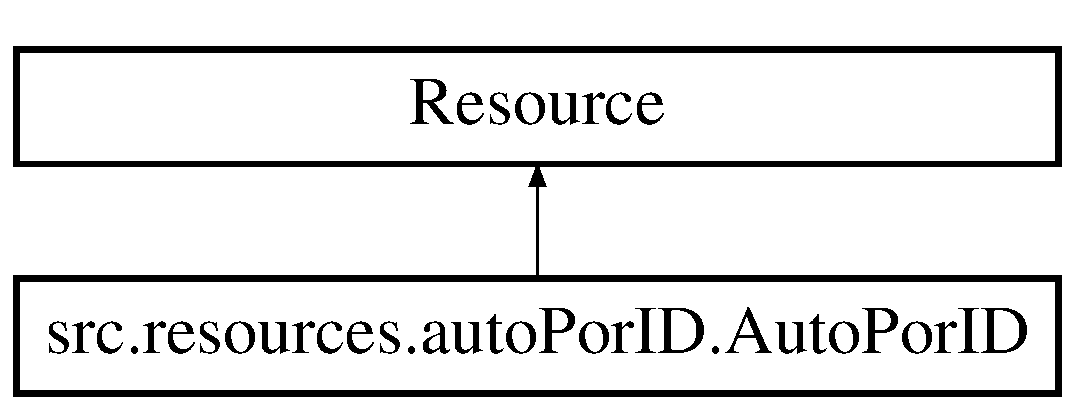
\includegraphics[height=2.000000cm]{classsrc_1_1resources_1_1auto_por_i_d_1_1_auto_por_i_d}
\end{center}
\end{figure}
\subsection*{Métodos públicos}
\begin{DoxyCompactItemize}
\item 
\hypertarget{classsrc_1_1resources_1_1auto_por_i_d_1_1_auto_por_i_d_a2446724f31d69e60ffb2b866609499f6}{def {\bfseries \-\_\-\-\_\-init\-\_\-\-\_\-}}\label{classsrc_1_1resources_1_1auto_por_i_d_1_1_auto_por_i_d_a2446724f31d69e60ffb2b866609499f6}

\item 
def \hyperlink{classsrc_1_1resources_1_1auto_por_i_d_1_1_auto_por_i_d_a29f36e323532a28e015bbe60b353837d}{get}
\begin{DoxyCompactList}\small\item\em Obtiene los datos de un auto de un conductor. \end{DoxyCompactList}\end{DoxyCompactItemize}
\subsection*{Atributos públicos}
\begin{DoxyCompactItemize}
\item 
\hypertarget{classsrc_1_1resources_1_1auto_por_i_d_1_1_auto_por_i_d_a0c36cdf16a521489f5145f46abe15dd2}{{\bfseries autenticador}}\label{classsrc_1_1resources_1_1auto_por_i_d_1_1_auto_por_i_d_a0c36cdf16a521489f5145f46abe15dd2}

\end{DoxyCompactItemize}
\subsection*{Métodos privados}
\begin{DoxyCompactItemize}
\item 
def \hyperlink{classsrc_1_1resources_1_1auto_por_i_d_1_1_auto_por_i_d_a227dddfb3e2156a084f85a23b2ddcf6d}{\-\_\-validar\-\_\-token}
\begin{DoxyCompactList}\small\item\em Valida al usuario. \end{DoxyCompactList}\item 
def \hyperlink{classsrc_1_1resources_1_1auto_por_i_d_1_1_auto_por_i_d_a22de3a2bd3a5024a6875e5683ddb491c}{\-\_\-acondicionar\-J\-S\-O\-N}
\begin{DoxyCompactList}\small\item\em Acondiciona un solo auto pasado. \end{DoxyCompactList}\end{DoxyCompactItemize}


\subsection{Descripción detallada}
Clase para la busqueda de un auto de un conductor. 



\subsection{Documentación de las funciones miembro}
\hypertarget{classsrc_1_1resources_1_1auto_por_i_d_1_1_auto_por_i_d_a22de3a2bd3a5024a6875e5683ddb491c}{\index{src\-::resources\-::auto\-Por\-I\-D\-::\-Auto\-Por\-I\-D@{src\-::resources\-::auto\-Por\-I\-D\-::\-Auto\-Por\-I\-D}!\-\_\-acondicionar\-J\-S\-O\-N@{\-\_\-acondicionar\-J\-S\-O\-N}}
\index{\-\_\-acondicionar\-J\-S\-O\-N@{\-\_\-acondicionar\-J\-S\-O\-N}!src::resources::autoPorID::AutoPorID@{src\-::resources\-::auto\-Por\-I\-D\-::\-Auto\-Por\-I\-D}}
\subsubsection[{\-\_\-acondicionar\-J\-S\-O\-N}]{\setlength{\rightskip}{0pt plus 5cm}def src.\-resources.\-auto\-Por\-I\-D.\-Auto\-Por\-I\-D.\-\_\-acondicionar\-J\-S\-O\-N (
\begin{DoxyParamCaption}
\item[{}]{self, }
\item[{}]{datos, }
\item[{}]{I\-D\-Usuario}
\end{DoxyParamCaption}
)\hspace{0.3cm}{\ttfamily [private]}}}\label{classsrc_1_1resources_1_1auto_por_i_d_1_1_auto_por_i_d_a22de3a2bd3a5024a6875e5683ddb491c}


Acondiciona un solo auto pasado. 


\begin{DoxyParams}{Parámetros}
{\em datos} & Es el auto a acondicionar. \\
\hline
\end{DoxyParams}
\hypertarget{classsrc_1_1resources_1_1auto_por_i_d_1_1_auto_por_i_d_a227dddfb3e2156a084f85a23b2ddcf6d}{\index{src\-::resources\-::auto\-Por\-I\-D\-::\-Auto\-Por\-I\-D@{src\-::resources\-::auto\-Por\-I\-D\-::\-Auto\-Por\-I\-D}!\-\_\-validar\-\_\-token@{\-\_\-validar\-\_\-token}}
\index{\-\_\-validar\-\_\-token@{\-\_\-validar\-\_\-token}!src::resources::autoPorID::AutoPorID@{src\-::resources\-::auto\-Por\-I\-D\-::\-Auto\-Por\-I\-D}}
\subsubsection[{\-\_\-validar\-\_\-token}]{\setlength{\rightskip}{0pt plus 5cm}def src.\-resources.\-auto\-Por\-I\-D.\-Auto\-Por\-I\-D.\-\_\-validar\-\_\-token (
\begin{DoxyParamCaption}
\item[{}]{self}
\end{DoxyParamCaption}
)\hspace{0.3cm}{\ttfamily [private]}}}\label{classsrc_1_1resources_1_1auto_por_i_d_1_1_auto_por_i_d_a227dddfb3e2156a084f85a23b2ddcf6d}


Valida al usuario. 

\hypertarget{classsrc_1_1resources_1_1auto_por_i_d_1_1_auto_por_i_d_a29f36e323532a28e015bbe60b353837d}{\index{src\-::resources\-::auto\-Por\-I\-D\-::\-Auto\-Por\-I\-D@{src\-::resources\-::auto\-Por\-I\-D\-::\-Auto\-Por\-I\-D}!get@{get}}
\index{get@{get}!src::resources::autoPorID::AutoPorID@{src\-::resources\-::auto\-Por\-I\-D\-::\-Auto\-Por\-I\-D}}
\subsubsection[{get}]{\setlength{\rightskip}{0pt plus 5cm}def src.\-resources.\-auto\-Por\-I\-D.\-Auto\-Por\-I\-D.\-get (
\begin{DoxyParamCaption}
\item[{}]{self, }
\item[{}]{I\-D\-Usuario, }
\item[{}]{I\-D\-Auto}
\end{DoxyParamCaption}
)}}\label{classsrc_1_1resources_1_1auto_por_i_d_1_1_auto_por_i_d_a29f36e323532a28e015bbe60b353837d}


Obtiene los datos de un auto de un conductor. 



La documentación para esta clase fue generada a partir del siguiente fichero\-:\begin{DoxyCompactItemize}
\item 
src/resources/auto\-Por\-I\-D.\-py\end{DoxyCompactItemize}

\hypertarget{classsrc_1_1resources_1_1autos_por_posicion_cercana_1_1_autos_por_posicion_cercana}{\section{Referencia de la Clase src.\-resources.\-autos\-Por\-Posicion\-Cercana.\-Autos\-Por\-Posicion\-Cercana}
\label{classsrc_1_1resources_1_1autos_por_posicion_cercana_1_1_autos_por_posicion_cercana}\index{src.\-resources.\-autos\-Por\-Posicion\-Cercana.\-Autos\-Por\-Posicion\-Cercana@{src.\-resources.\-autos\-Por\-Posicion\-Cercana.\-Autos\-Por\-Posicion\-Cercana}}
}


Clase para la busqueda de autos de usuarios.  


Diagrama de herencias de src.\-resources.\-autos\-Por\-Posicion\-Cercana.\-Autos\-Por\-Posicion\-Cercana\begin{figure}[H]
\begin{center}
\leavevmode
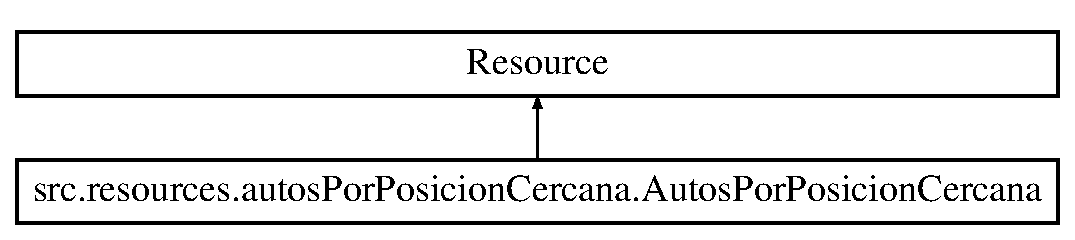
\includegraphics[height=2.000000cm]{classsrc_1_1resources_1_1autos_por_posicion_cercana_1_1_autos_por_posicion_cercana}
\end{center}
\end{figure}
\subsection*{Métodos públicos}
\begin{DoxyCompactItemize}
\item 
\hypertarget{classsrc_1_1resources_1_1autos_por_posicion_cercana_1_1_autos_por_posicion_cercana_ab915321f8adc8b09dca3e6b2a289eedf}{def {\bfseries \-\_\-\-\_\-init\-\_\-\-\_\-}}\label{classsrc_1_1resources_1_1autos_por_posicion_cercana_1_1_autos_por_posicion_cercana_ab915321f8adc8b09dca3e6b2a289eedf}

\item 
def \hyperlink{classsrc_1_1resources_1_1autos_por_posicion_cercana_1_1_autos_por_posicion_cercana_a5411713030f29c3612462e582af92b90}{get}
\begin{DoxyCompactList}\small\item\em Obtiene los conductores cercanos a un determinado usuario. \end{DoxyCompactList}\end{DoxyCompactItemize}
\subsection*{Atributos públicos}
\begin{DoxyCompactItemize}
\item 
\hypertarget{classsrc_1_1resources_1_1autos_por_posicion_cercana_1_1_autos_por_posicion_cercana_a377d6bb97dc7f9be4e429c4f05bcb17f}{{\bfseries autenticador}}\label{classsrc_1_1resources_1_1autos_por_posicion_cercana_1_1_autos_por_posicion_cercana_a377d6bb97dc7f9be4e429c4f05bcb17f}

\item 
\hypertarget{classsrc_1_1resources_1_1autos_por_posicion_cercana_1_1_autos_por_posicion_cercana_ab44f49d52500f775a36b7a5983127250}{{\bfseries distancia\-Maxima}}\label{classsrc_1_1resources_1_1autos_por_posicion_cercana_1_1_autos_por_posicion_cercana_ab44f49d52500f775a36b7a5983127250}

\end{DoxyCompactItemize}
\subsection*{Métodos privados}
\begin{DoxyCompactItemize}
\item 
def \hyperlink{classsrc_1_1resources_1_1autos_por_posicion_cercana_1_1_autos_por_posicion_cercana_a651a21fe70cdb11ccb7ecddf3a2ef71e}{\-\_\-get\-\_\-param\-\_\-from\-\_\-request}
\begin{DoxyCompactList}\small\item\em Obtiene el parametro dado de la request. \end{DoxyCompactList}\item 
def \hyperlink{classsrc_1_1resources_1_1autos_por_posicion_cercana_1_1_autos_por_posicion_cercana_af31560b90a07c4caf7dcd7f729a97473}{\-\_\-validate\-\_\-get\-\_\-request}
\begin{DoxyCompactList}\small\item\em Tiene que estar la posicion del usuario que realiza la busqueda. \end{DoxyCompactList}\item 
def \hyperlink{classsrc_1_1resources_1_1autos_por_posicion_cercana_1_1_autos_por_posicion_cercana_a071a3bedc7dabbdcfa7a3a2c72ccfb04}{\-\_\-validar\-\_\-token}
\begin{DoxyCompactList}\small\item\em Valida al usuario. \end{DoxyCompactList}\item 
def \hyperlink{classsrc_1_1resources_1_1autos_por_posicion_cercana_1_1_autos_por_posicion_cercana_ae2a7c1697a8d0b5e263a8178f3ad9352}{\-\_\-obtener\-\_\-autos\-\_\-cercanos}
\begin{DoxyCompactList}\small\item\em Obtiene los autos cercanos que tenga registrados en mongo\-D\-B. \end{DoxyCompactList}\item 
def \hyperlink{classsrc_1_1resources_1_1autos_por_posicion_cercana_1_1_autos_por_posicion_cercana_a087e0b7b45211aff9925ce9fdcd368bc}{\-\_\-acondicionar\-Auto\-J\-S\-O\-N}
\begin{DoxyCompactList}\small\item\em Acondiciona un solo auto pasado. \end{DoxyCompactList}\item 
def \hyperlink{classsrc_1_1resources_1_1autos_por_posicion_cercana_1_1_autos_por_posicion_cercana_aa2d6fe08fd52d4fd16b9d6c1831a0d2b}{\-\_\-acondicionar\-J\-S\-O\-N}
\begin{DoxyCompactList}\small\item\em Itera en los autos y arma el J\-S\-O\-N. \end{DoxyCompactList}\end{DoxyCompactItemize}


\subsection{Descripción detallada}
Clase para la busqueda de autos de usuarios. 



\subsection{Documentación de las funciones miembro}
\hypertarget{classsrc_1_1resources_1_1autos_por_posicion_cercana_1_1_autos_por_posicion_cercana_a087e0b7b45211aff9925ce9fdcd368bc}{\index{src\-::resources\-::autos\-Por\-Posicion\-Cercana\-::\-Autos\-Por\-Posicion\-Cercana@{src\-::resources\-::autos\-Por\-Posicion\-Cercana\-::\-Autos\-Por\-Posicion\-Cercana}!\-\_\-acondicionar\-Auto\-J\-S\-O\-N@{\-\_\-acondicionar\-Auto\-J\-S\-O\-N}}
\index{\-\_\-acondicionar\-Auto\-J\-S\-O\-N@{\-\_\-acondicionar\-Auto\-J\-S\-O\-N}!src::resources::autosPorPosicionCercana::AutosPorPosicionCercana@{src\-::resources\-::autos\-Por\-Posicion\-Cercana\-::\-Autos\-Por\-Posicion\-Cercana}}
\subsubsection[{\-\_\-acondicionar\-Auto\-J\-S\-O\-N}]{\setlength{\rightskip}{0pt plus 5cm}def src.\-resources.\-autos\-Por\-Posicion\-Cercana.\-Autos\-Por\-Posicion\-Cercana.\-\_\-acondicionar\-Auto\-J\-S\-O\-N (
\begin{DoxyParamCaption}
\item[{}]{self, }
\item[{}]{datos}
\end{DoxyParamCaption}
)\hspace{0.3cm}{\ttfamily [private]}}}\label{classsrc_1_1resources_1_1autos_por_posicion_cercana_1_1_autos_por_posicion_cercana_a087e0b7b45211aff9925ce9fdcd368bc}


Acondiciona un solo auto pasado. 


\begin{DoxyParams}{Parámetros}
{\em datos} & Es el auto a acondicionar. \begin{DoxyVerb}Le pide los datos al Shared Server.\end{DoxyVerb}
 \\
\hline
\end{DoxyParams}
\hypertarget{classsrc_1_1resources_1_1autos_por_posicion_cercana_1_1_autos_por_posicion_cercana_aa2d6fe08fd52d4fd16b9d6c1831a0d2b}{\index{src\-::resources\-::autos\-Por\-Posicion\-Cercana\-::\-Autos\-Por\-Posicion\-Cercana@{src\-::resources\-::autos\-Por\-Posicion\-Cercana\-::\-Autos\-Por\-Posicion\-Cercana}!\-\_\-acondicionar\-J\-S\-O\-N@{\-\_\-acondicionar\-J\-S\-O\-N}}
\index{\-\_\-acondicionar\-J\-S\-O\-N@{\-\_\-acondicionar\-J\-S\-O\-N}!src::resources::autosPorPosicionCercana::AutosPorPosicionCercana@{src\-::resources\-::autos\-Por\-Posicion\-Cercana\-::\-Autos\-Por\-Posicion\-Cercana}}
\subsubsection[{\-\_\-acondicionar\-J\-S\-O\-N}]{\setlength{\rightskip}{0pt plus 5cm}def src.\-resources.\-autos\-Por\-Posicion\-Cercana.\-Autos\-Por\-Posicion\-Cercana.\-\_\-acondicionar\-J\-S\-O\-N (
\begin{DoxyParamCaption}
\item[{}]{self, }
\item[{}]{datos}
\end{DoxyParamCaption}
)\hspace{0.3cm}{\ttfamily [private]}}}\label{classsrc_1_1resources_1_1autos_por_posicion_cercana_1_1_autos_por_posicion_cercana_aa2d6fe08fd52d4fd16b9d6c1831a0d2b}


Itera en los autos y arma el J\-S\-O\-N. 


\begin{DoxyParams}{Parámetros}
{\em datos} & La response que se obtuvo de mongo\-D\-B. \\
\hline
\end{DoxyParams}
\hypertarget{classsrc_1_1resources_1_1autos_por_posicion_cercana_1_1_autos_por_posicion_cercana_a651a21fe70cdb11ccb7ecddf3a2ef71e}{\index{src\-::resources\-::autos\-Por\-Posicion\-Cercana\-::\-Autos\-Por\-Posicion\-Cercana@{src\-::resources\-::autos\-Por\-Posicion\-Cercana\-::\-Autos\-Por\-Posicion\-Cercana}!\-\_\-get\-\_\-param\-\_\-from\-\_\-request@{\-\_\-get\-\_\-param\-\_\-from\-\_\-request}}
\index{\-\_\-get\-\_\-param\-\_\-from\-\_\-request@{\-\_\-get\-\_\-param\-\_\-from\-\_\-request}!src::resources::autosPorPosicionCercana::AutosPorPosicionCercana@{src\-::resources\-::autos\-Por\-Posicion\-Cercana\-::\-Autos\-Por\-Posicion\-Cercana}}
\subsubsection[{\-\_\-get\-\_\-param\-\_\-from\-\_\-request}]{\setlength{\rightskip}{0pt plus 5cm}def src.\-resources.\-autos\-Por\-Posicion\-Cercana.\-Autos\-Por\-Posicion\-Cercana.\-\_\-get\-\_\-param\-\_\-from\-\_\-request (
\begin{DoxyParamCaption}
\item[{}]{self, }
\item[{}]{nombre\-Parametro}
\end{DoxyParamCaption}
)\hspace{0.3cm}{\ttfamily [private]}}}\label{classsrc_1_1resources_1_1autos_por_posicion_cercana_1_1_autos_por_posicion_cercana_a651a21fe70cdb11ccb7ecddf3a2ef71e}


Obtiene el parametro dado de la request. 

\hypertarget{classsrc_1_1resources_1_1autos_por_posicion_cercana_1_1_autos_por_posicion_cercana_ae2a7c1697a8d0b5e263a8178f3ad9352}{\index{src\-::resources\-::autos\-Por\-Posicion\-Cercana\-::\-Autos\-Por\-Posicion\-Cercana@{src\-::resources\-::autos\-Por\-Posicion\-Cercana\-::\-Autos\-Por\-Posicion\-Cercana}!\-\_\-obtener\-\_\-autos\-\_\-cercanos@{\-\_\-obtener\-\_\-autos\-\_\-cercanos}}
\index{\-\_\-obtener\-\_\-autos\-\_\-cercanos@{\-\_\-obtener\-\_\-autos\-\_\-cercanos}!src::resources::autosPorPosicionCercana::AutosPorPosicionCercana@{src\-::resources\-::autos\-Por\-Posicion\-Cercana\-::\-Autos\-Por\-Posicion\-Cercana}}
\subsubsection[{\-\_\-obtener\-\_\-autos\-\_\-cercanos}]{\setlength{\rightskip}{0pt plus 5cm}def src.\-resources.\-autos\-Por\-Posicion\-Cercana.\-Autos\-Por\-Posicion\-Cercana.\-\_\-obtener\-\_\-autos\-\_\-cercanos (
\begin{DoxyParamCaption}
\item[{}]{self, }
\item[{}]{x, }
\item[{}]{y}
\end{DoxyParamCaption}
)\hspace{0.3cm}{\ttfamily [private]}}}\label{classsrc_1_1resources_1_1autos_por_posicion_cercana_1_1_autos_por_posicion_cercana_ae2a7c1697a8d0b5e263a8178f3ad9352}


Obtiene los autos cercanos que tenga registrados en mongo\-D\-B. 

\begin{DoxyVerb}Convierte a metros\end{DoxyVerb}
 \hypertarget{classsrc_1_1resources_1_1autos_por_posicion_cercana_1_1_autos_por_posicion_cercana_a071a3bedc7dabbdcfa7a3a2c72ccfb04}{\index{src\-::resources\-::autos\-Por\-Posicion\-Cercana\-::\-Autos\-Por\-Posicion\-Cercana@{src\-::resources\-::autos\-Por\-Posicion\-Cercana\-::\-Autos\-Por\-Posicion\-Cercana}!\-\_\-validar\-\_\-token@{\-\_\-validar\-\_\-token}}
\index{\-\_\-validar\-\_\-token@{\-\_\-validar\-\_\-token}!src::resources::autosPorPosicionCercana::AutosPorPosicionCercana@{src\-::resources\-::autos\-Por\-Posicion\-Cercana\-::\-Autos\-Por\-Posicion\-Cercana}}
\subsubsection[{\-\_\-validar\-\_\-token}]{\setlength{\rightskip}{0pt plus 5cm}def src.\-resources.\-autos\-Por\-Posicion\-Cercana.\-Autos\-Por\-Posicion\-Cercana.\-\_\-validar\-\_\-token (
\begin{DoxyParamCaption}
\item[{}]{self}
\end{DoxyParamCaption}
)\hspace{0.3cm}{\ttfamily [private]}}}\label{classsrc_1_1resources_1_1autos_por_posicion_cercana_1_1_autos_por_posicion_cercana_a071a3bedc7dabbdcfa7a3a2c72ccfb04}


Valida al usuario. 

\hypertarget{classsrc_1_1resources_1_1autos_por_posicion_cercana_1_1_autos_por_posicion_cercana_af31560b90a07c4caf7dcd7f729a97473}{\index{src\-::resources\-::autos\-Por\-Posicion\-Cercana\-::\-Autos\-Por\-Posicion\-Cercana@{src\-::resources\-::autos\-Por\-Posicion\-Cercana\-::\-Autos\-Por\-Posicion\-Cercana}!\-\_\-validate\-\_\-get\-\_\-request@{\-\_\-validate\-\_\-get\-\_\-request}}
\index{\-\_\-validate\-\_\-get\-\_\-request@{\-\_\-validate\-\_\-get\-\_\-request}!src::resources::autosPorPosicionCercana::AutosPorPosicionCercana@{src\-::resources\-::autos\-Por\-Posicion\-Cercana\-::\-Autos\-Por\-Posicion\-Cercana}}
\subsubsection[{\-\_\-validate\-\_\-get\-\_\-request}]{\setlength{\rightskip}{0pt plus 5cm}def src.\-resources.\-autos\-Por\-Posicion\-Cercana.\-Autos\-Por\-Posicion\-Cercana.\-\_\-validate\-\_\-get\-\_\-request (
\begin{DoxyParamCaption}
\item[{}]{self}
\end{DoxyParamCaption}
)\hspace{0.3cm}{\ttfamily [private]}}}\label{classsrc_1_1resources_1_1autos_por_posicion_cercana_1_1_autos_por_posicion_cercana_af31560b90a07c4caf7dcd7f729a97473}


Tiene que estar la posicion del usuario que realiza la busqueda. 

\hypertarget{classsrc_1_1resources_1_1autos_por_posicion_cercana_1_1_autos_por_posicion_cercana_a5411713030f29c3612462e582af92b90}{\index{src\-::resources\-::autos\-Por\-Posicion\-Cercana\-::\-Autos\-Por\-Posicion\-Cercana@{src\-::resources\-::autos\-Por\-Posicion\-Cercana\-::\-Autos\-Por\-Posicion\-Cercana}!get@{get}}
\index{get@{get}!src::resources::autosPorPosicionCercana::AutosPorPosicionCercana@{src\-::resources\-::autos\-Por\-Posicion\-Cercana\-::\-Autos\-Por\-Posicion\-Cercana}}
\subsubsection[{get}]{\setlength{\rightskip}{0pt plus 5cm}def src.\-resources.\-autos\-Por\-Posicion\-Cercana.\-Autos\-Por\-Posicion\-Cercana.\-get (
\begin{DoxyParamCaption}
\item[{}]{self}
\end{DoxyParamCaption}
)}}\label{classsrc_1_1resources_1_1autos_por_posicion_cercana_1_1_autos_por_posicion_cercana_a5411713030f29c3612462e582af92b90}


Obtiene los conductores cercanos a un determinado usuario. 



La documentación para esta clase fue generada a partir del siguiente fichero\-:\begin{DoxyCompactItemize}
\item 
src/resources/autos\-Por\-Posicion\-Cercana.\-py\end{DoxyCompactItemize}

\hypertarget{classsrc_1_1resources_1_1autos_por_usuario_1_1_autos_por_usuario}{\section{Referencia de la Clase src.\-resources.\-autos\-Por\-Usuario.\-Autos\-Por\-Usuario}
\label{classsrc_1_1resources_1_1autos_por_usuario_1_1_autos_por_usuario}\index{src.\-resources.\-autos\-Por\-Usuario.\-Autos\-Por\-Usuario@{src.\-resources.\-autos\-Por\-Usuario.\-Autos\-Por\-Usuario}}
}


Clase para la busqueda de autos de un usuario.  


Diagrama de herencias de src.\-resources.\-autos\-Por\-Usuario.\-Autos\-Por\-Usuario\begin{figure}[H]
\begin{center}
\leavevmode
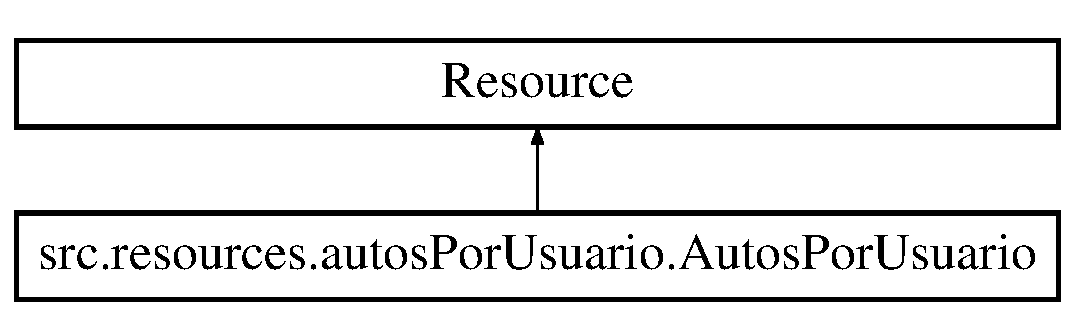
\includegraphics[height=2.000000cm]{classsrc_1_1resources_1_1autos_por_usuario_1_1_autos_por_usuario}
\end{center}
\end{figure}
\subsection*{Métodos públicos}
\begin{DoxyCompactItemize}
\item 
\hypertarget{classsrc_1_1resources_1_1autos_por_usuario_1_1_autos_por_usuario_a4ef31d25c8eaa7ec535645d7d62b85c5}{def {\bfseries \-\_\-\-\_\-init\-\_\-\-\_\-}}\label{classsrc_1_1resources_1_1autos_por_usuario_1_1_autos_por_usuario_a4ef31d25c8eaa7ec535645d7d62b85c5}

\item 
def \hyperlink{classsrc_1_1resources_1_1autos_por_usuario_1_1_autos_por_usuario_a2114ca03b2dc41a64af704b59609e791}{get}
\begin{DoxyCompactList}\small\item\em Obtiene los autos de un determinado conductor. \end{DoxyCompactList}\end{DoxyCompactItemize}
\subsection*{Atributos públicos}
\begin{DoxyCompactItemize}
\item 
\hypertarget{classsrc_1_1resources_1_1autos_por_usuario_1_1_autos_por_usuario_aeec994ebf06f73c686dd5560da3add73}{{\bfseries autenticador}}\label{classsrc_1_1resources_1_1autos_por_usuario_1_1_autos_por_usuario_aeec994ebf06f73c686dd5560da3add73}

\end{DoxyCompactItemize}
\subsection*{Métodos privados}
\begin{DoxyCompactItemize}
\item 
def \hyperlink{classsrc_1_1resources_1_1autos_por_usuario_1_1_autos_por_usuario_adec61b4d99af1d8a37538e36572a047f}{\-\_\-validar\-\_\-token}
\begin{DoxyCompactList}\small\item\em Valida al usuario. \end{DoxyCompactList}\item 
def \hyperlink{classsrc_1_1resources_1_1autos_por_usuario_1_1_autos_por_usuario_ab536a2b91c380db5d95b8f88857fa4f4}{\-\_\-acondicionar\-Auto\-J\-S\-O\-N}
\begin{DoxyCompactList}\small\item\em Acondiciona un solo auto pasado. \end{DoxyCompactList}\item 
def \hyperlink{classsrc_1_1resources_1_1autos_por_usuario_1_1_autos_por_usuario_a31c3ea98b38c88058e0036d95d06bd8c}{\-\_\-acondicionar\-J\-S\-O\-N}
\begin{DoxyCompactList}\small\item\em Itera en los autos y arma el J\-S\-O\-N. \end{DoxyCompactList}\end{DoxyCompactItemize}


\subsection{Descripción detallada}
Clase para la busqueda de autos de un usuario. 



\subsection{Documentación de las funciones miembro}
\hypertarget{classsrc_1_1resources_1_1autos_por_usuario_1_1_autos_por_usuario_ab536a2b91c380db5d95b8f88857fa4f4}{\index{src\-::resources\-::autos\-Por\-Usuario\-::\-Autos\-Por\-Usuario@{src\-::resources\-::autos\-Por\-Usuario\-::\-Autos\-Por\-Usuario}!\-\_\-acondicionar\-Auto\-J\-S\-O\-N@{\-\_\-acondicionar\-Auto\-J\-S\-O\-N}}
\index{\-\_\-acondicionar\-Auto\-J\-S\-O\-N@{\-\_\-acondicionar\-Auto\-J\-S\-O\-N}!src::resources::autosPorUsuario::AutosPorUsuario@{src\-::resources\-::autos\-Por\-Usuario\-::\-Autos\-Por\-Usuario}}
\subsubsection[{\-\_\-acondicionar\-Auto\-J\-S\-O\-N}]{\setlength{\rightskip}{0pt plus 5cm}def src.\-resources.\-autos\-Por\-Usuario.\-Autos\-Por\-Usuario.\-\_\-acondicionar\-Auto\-J\-S\-O\-N (
\begin{DoxyParamCaption}
\item[{}]{self, }
\item[{}]{datos, }
\item[{}]{es\-Auto\-Activo}
\end{DoxyParamCaption}
)\hspace{0.3cm}{\ttfamily [private]}}}\label{classsrc_1_1resources_1_1autos_por_usuario_1_1_autos_por_usuario_ab536a2b91c380db5d95b8f88857fa4f4}


Acondiciona un solo auto pasado. 


\begin{DoxyParams}{Parámetros}
{\em datos} & Es el auto a acondicionar. \\
\hline
\end{DoxyParams}
\hypertarget{classsrc_1_1resources_1_1autos_por_usuario_1_1_autos_por_usuario_a31c3ea98b38c88058e0036d95d06bd8c}{\index{src\-::resources\-::autos\-Por\-Usuario\-::\-Autos\-Por\-Usuario@{src\-::resources\-::autos\-Por\-Usuario\-::\-Autos\-Por\-Usuario}!\-\_\-acondicionar\-J\-S\-O\-N@{\-\_\-acondicionar\-J\-S\-O\-N}}
\index{\-\_\-acondicionar\-J\-S\-O\-N@{\-\_\-acondicionar\-J\-S\-O\-N}!src::resources::autosPorUsuario::AutosPorUsuario@{src\-::resources\-::autos\-Por\-Usuario\-::\-Autos\-Por\-Usuario}}
\subsubsection[{\-\_\-acondicionar\-J\-S\-O\-N}]{\setlength{\rightskip}{0pt plus 5cm}def src.\-resources.\-autos\-Por\-Usuario.\-Autos\-Por\-Usuario.\-\_\-acondicionar\-J\-S\-O\-N (
\begin{DoxyParamCaption}
\item[{}]{self, }
\item[{}]{datos, }
\item[{}]{I\-D\-Usuario}
\end{DoxyParamCaption}
)\hspace{0.3cm}{\ttfamily [private]}}}\label{classsrc_1_1resources_1_1autos_por_usuario_1_1_autos_por_usuario_a31c3ea98b38c88058e0036d95d06bd8c}


Itera en los autos y arma el J\-S\-O\-N. 


\begin{DoxyParams}{Parámetros}
{\em datos} & La response que se obtuvo del Shared Server. \\
\hline
\end{DoxyParams}
\hypertarget{classsrc_1_1resources_1_1autos_por_usuario_1_1_autos_por_usuario_adec61b4d99af1d8a37538e36572a047f}{\index{src\-::resources\-::autos\-Por\-Usuario\-::\-Autos\-Por\-Usuario@{src\-::resources\-::autos\-Por\-Usuario\-::\-Autos\-Por\-Usuario}!\-\_\-validar\-\_\-token@{\-\_\-validar\-\_\-token}}
\index{\-\_\-validar\-\_\-token@{\-\_\-validar\-\_\-token}!src::resources::autosPorUsuario::AutosPorUsuario@{src\-::resources\-::autos\-Por\-Usuario\-::\-Autos\-Por\-Usuario}}
\subsubsection[{\-\_\-validar\-\_\-token}]{\setlength{\rightskip}{0pt plus 5cm}def src.\-resources.\-autos\-Por\-Usuario.\-Autos\-Por\-Usuario.\-\_\-validar\-\_\-token (
\begin{DoxyParamCaption}
\item[{}]{self}
\end{DoxyParamCaption}
)\hspace{0.3cm}{\ttfamily [private]}}}\label{classsrc_1_1resources_1_1autos_por_usuario_1_1_autos_por_usuario_adec61b4d99af1d8a37538e36572a047f}


Valida al usuario. 

\hypertarget{classsrc_1_1resources_1_1autos_por_usuario_1_1_autos_por_usuario_a2114ca03b2dc41a64af704b59609e791}{\index{src\-::resources\-::autos\-Por\-Usuario\-::\-Autos\-Por\-Usuario@{src\-::resources\-::autos\-Por\-Usuario\-::\-Autos\-Por\-Usuario}!get@{get}}
\index{get@{get}!src::resources::autosPorUsuario::AutosPorUsuario@{src\-::resources\-::autos\-Por\-Usuario\-::\-Autos\-Por\-Usuario}}
\subsubsection[{get}]{\setlength{\rightskip}{0pt plus 5cm}def src.\-resources.\-autos\-Por\-Usuario.\-Autos\-Por\-Usuario.\-get (
\begin{DoxyParamCaption}
\item[{}]{self, }
\item[{}]{I\-D\-Usuario}
\end{DoxyParamCaption}
)}}\label{classsrc_1_1resources_1_1autos_por_usuario_1_1_autos_por_usuario_a2114ca03b2dc41a64af704b59609e791}


Obtiene los autos de un determinado conductor. 



La documentación para esta clase fue generada a partir del siguiente fichero\-:\begin{DoxyCompactItemize}
\item 
src/resources/autos\-Por\-Usuario.\-py\end{DoxyCompactItemize}

\hypertarget{classsrc_1_1resources_1_1driver_modificar_posicion_1_1_conductor_modificar_posicion}{\section{Referencia de la Clase src.\-resources.\-driver\-Modificar\-Posicion.\-Conductor\-Modificar\-Posicion}
\label{classsrc_1_1resources_1_1driver_modificar_posicion_1_1_conductor_modificar_posicion}\index{src.\-resources.\-driver\-Modificar\-Posicion.\-Conductor\-Modificar\-Posicion@{src.\-resources.\-driver\-Modificar\-Posicion.\-Conductor\-Modificar\-Posicion}}
}


Clase para actualizar la posicion de un conductor.  


Diagrama de herencias de src.\-resources.\-driver\-Modificar\-Posicion.\-Conductor\-Modificar\-Posicion\begin{figure}[H]
\begin{center}
\leavevmode
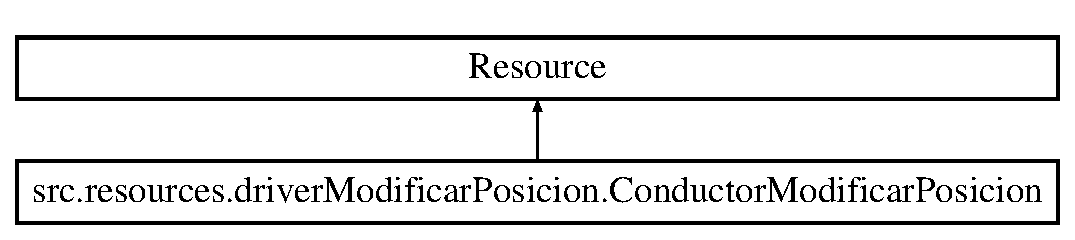
\includegraphics[height=2.000000cm]{classsrc_1_1resources_1_1driver_modificar_posicion_1_1_conductor_modificar_posicion}
\end{center}
\end{figure}
\subsection*{Métodos públicos}
\begin{DoxyCompactItemize}
\item 
\hypertarget{classsrc_1_1resources_1_1driver_modificar_posicion_1_1_conductor_modificar_posicion_a54c8ffdffc9d1a7057ec8fea60b6c92f}{def {\bfseries \-\_\-\-\_\-init\-\_\-\-\_\-}}\label{classsrc_1_1resources_1_1driver_modificar_posicion_1_1_conductor_modificar_posicion_a54c8ffdffc9d1a7057ec8fea60b6c92f}

\item 
def \hyperlink{classsrc_1_1resources_1_1driver_modificar_posicion_1_1_conductor_modificar_posicion_a93cfdaaee4b2f167fff1a96f5b2924d7}{put}
\begin{DoxyCompactList}\small\item\em Actualiza los datos de posicion de un conductor. \end{DoxyCompactList}\end{DoxyCompactItemize}
\subsection*{Atributos públicos}
\begin{DoxyCompactItemize}
\item 
\hypertarget{classsrc_1_1resources_1_1driver_modificar_posicion_1_1_conductor_modificar_posicion_a2c579ca60058f1ba721ee7a06390e094}{{\bfseries autenticador}}\label{classsrc_1_1resources_1_1driver_modificar_posicion_1_1_conductor_modificar_posicion_a2c579ca60058f1ba721ee7a06390e094}

\end{DoxyCompactItemize}
\subsection*{Métodos privados}
\begin{DoxyCompactItemize}
\item 
def \hyperlink{classsrc_1_1resources_1_1driver_modificar_posicion_1_1_conductor_modificar_posicion_aeb0a85b50e4dff9aadf447c18e047927}{\-\_\-get\-\_\-data\-\_\-from\-\_\-request}
\begin{DoxyCompactList}\small\item\em Obtiene la propiedad del json contenido de la request. \end{DoxyCompactList}\item 
def \hyperlink{classsrc_1_1resources_1_1driver_modificar_posicion_1_1_conductor_modificar_posicion_ab108939cbeb442ef668b9e9a3f73256b}{\-\_\-validate\-\_\-request}
\begin{DoxyCompactList}\small\item\em Valida que haya una request completa. \end{DoxyCompactList}\item 
def \hyperlink{classsrc_1_1resources_1_1driver_modificar_posicion_1_1_conductor_modificar_posicion_ac748fc1e6dadb7fb7c12e21bc83d9bfa}{\-\_\-validar\-\_\-token}
\begin{DoxyCompactList}\small\item\em Valida al usuario. \end{DoxyCompactList}\item 
def \hyperlink{classsrc_1_1resources_1_1driver_modificar_posicion_1_1_conductor_modificar_posicion_afef21f0ec8f37cda7789bcf231949ed5}{\-\_\-actualizar\-\_\-datos\-\_\-viaje}
\begin{DoxyCompactList}\small\item\em Modifica los parametros del viaje en curso si corresponde. \end{DoxyCompactList}\item 
\hypertarget{classsrc_1_1resources_1_1driver_modificar_posicion_1_1_conductor_modificar_posicion_a41f849ecba78284f88af9c50546d59b1}{def {\bfseries \-\_\-actualizar\-\_\-posicion\-\_\-conductor}}\label{classsrc_1_1resources_1_1driver_modificar_posicion_1_1_conductor_modificar_posicion_a41f849ecba78284f88af9c50546d59b1}

\end{DoxyCompactItemize}


\subsection{Descripción detallada}
Clase para actualizar la posicion de un conductor. 



\subsection{Documentación de las funciones miembro}
\hypertarget{classsrc_1_1resources_1_1driver_modificar_posicion_1_1_conductor_modificar_posicion_afef21f0ec8f37cda7789bcf231949ed5}{\index{src\-::resources\-::driver\-Modificar\-Posicion\-::\-Conductor\-Modificar\-Posicion@{src\-::resources\-::driver\-Modificar\-Posicion\-::\-Conductor\-Modificar\-Posicion}!\-\_\-actualizar\-\_\-datos\-\_\-viaje@{\-\_\-actualizar\-\_\-datos\-\_\-viaje}}
\index{\-\_\-actualizar\-\_\-datos\-\_\-viaje@{\-\_\-actualizar\-\_\-datos\-\_\-viaje}!src::resources::driverModificarPosicion::ConductorModificarPosicion@{src\-::resources\-::driver\-Modificar\-Posicion\-::\-Conductor\-Modificar\-Posicion}}
\subsubsection[{\-\_\-actualizar\-\_\-datos\-\_\-viaje}]{\setlength{\rightskip}{0pt plus 5cm}def src.\-resources.\-driver\-Modificar\-Posicion.\-Conductor\-Modificar\-Posicion.\-\_\-actualizar\-\_\-datos\-\_\-viaje (
\begin{DoxyParamCaption}
\item[{}]{self, }
\item[{}]{datos\-Conductor, }
\item[{}]{x, }
\item[{}]{y}
\end{DoxyParamCaption}
)\hspace{0.3cm}{\ttfamily [private]}}}\label{classsrc_1_1resources_1_1driver_modificar_posicion_1_1_conductor_modificar_posicion_afef21f0ec8f37cda7789bcf231949ed5}


Modifica los parametros del viaje en curso si corresponde. 

\hypertarget{classsrc_1_1resources_1_1driver_modificar_posicion_1_1_conductor_modificar_posicion_aeb0a85b50e4dff9aadf447c18e047927}{\index{src\-::resources\-::driver\-Modificar\-Posicion\-::\-Conductor\-Modificar\-Posicion@{src\-::resources\-::driver\-Modificar\-Posicion\-::\-Conductor\-Modificar\-Posicion}!\-\_\-get\-\_\-data\-\_\-from\-\_\-request@{\-\_\-get\-\_\-data\-\_\-from\-\_\-request}}
\index{\-\_\-get\-\_\-data\-\_\-from\-\_\-request@{\-\_\-get\-\_\-data\-\_\-from\-\_\-request}!src::resources::driverModificarPosicion::ConductorModificarPosicion@{src\-::resources\-::driver\-Modificar\-Posicion\-::\-Conductor\-Modificar\-Posicion}}
\subsubsection[{\-\_\-get\-\_\-data\-\_\-from\-\_\-request}]{\setlength{\rightskip}{0pt plus 5cm}def src.\-resources.\-driver\-Modificar\-Posicion.\-Conductor\-Modificar\-Posicion.\-\_\-get\-\_\-data\-\_\-from\-\_\-request (
\begin{DoxyParamCaption}
\item[{}]{self, }
\item[{}]{nombre\-Propiedad}
\end{DoxyParamCaption}
)\hspace{0.3cm}{\ttfamily [private]}}}\label{classsrc_1_1resources_1_1driver_modificar_posicion_1_1_conductor_modificar_posicion_aeb0a85b50e4dff9aadf447c18e047927}


Obtiene la propiedad del json contenido de la request. 

\hypertarget{classsrc_1_1resources_1_1driver_modificar_posicion_1_1_conductor_modificar_posicion_ac748fc1e6dadb7fb7c12e21bc83d9bfa}{\index{src\-::resources\-::driver\-Modificar\-Posicion\-::\-Conductor\-Modificar\-Posicion@{src\-::resources\-::driver\-Modificar\-Posicion\-::\-Conductor\-Modificar\-Posicion}!\-\_\-validar\-\_\-token@{\-\_\-validar\-\_\-token}}
\index{\-\_\-validar\-\_\-token@{\-\_\-validar\-\_\-token}!src::resources::driverModificarPosicion::ConductorModificarPosicion@{src\-::resources\-::driver\-Modificar\-Posicion\-::\-Conductor\-Modificar\-Posicion}}
\subsubsection[{\-\_\-validar\-\_\-token}]{\setlength{\rightskip}{0pt plus 5cm}def src.\-resources.\-driver\-Modificar\-Posicion.\-Conductor\-Modificar\-Posicion.\-\_\-validar\-\_\-token (
\begin{DoxyParamCaption}
\item[{}]{self}
\end{DoxyParamCaption}
)\hspace{0.3cm}{\ttfamily [private]}}}\label{classsrc_1_1resources_1_1driver_modificar_posicion_1_1_conductor_modificar_posicion_ac748fc1e6dadb7fb7c12e21bc83d9bfa}


Valida al usuario. 

\hypertarget{classsrc_1_1resources_1_1driver_modificar_posicion_1_1_conductor_modificar_posicion_ab108939cbeb442ef668b9e9a3f73256b}{\index{src\-::resources\-::driver\-Modificar\-Posicion\-::\-Conductor\-Modificar\-Posicion@{src\-::resources\-::driver\-Modificar\-Posicion\-::\-Conductor\-Modificar\-Posicion}!\-\_\-validate\-\_\-request@{\-\_\-validate\-\_\-request}}
\index{\-\_\-validate\-\_\-request@{\-\_\-validate\-\_\-request}!src::resources::driverModificarPosicion::ConductorModificarPosicion@{src\-::resources\-::driver\-Modificar\-Posicion\-::\-Conductor\-Modificar\-Posicion}}
\subsubsection[{\-\_\-validate\-\_\-request}]{\setlength{\rightskip}{0pt plus 5cm}def src.\-resources.\-driver\-Modificar\-Posicion.\-Conductor\-Modificar\-Posicion.\-\_\-validate\-\_\-request (
\begin{DoxyParamCaption}
\item[{}]{self}
\end{DoxyParamCaption}
)\hspace{0.3cm}{\ttfamily [private]}}}\label{classsrc_1_1resources_1_1driver_modificar_posicion_1_1_conductor_modificar_posicion_ab108939cbeb442ef668b9e9a3f73256b}


Valida que haya una request completa. 

\hypertarget{classsrc_1_1resources_1_1driver_modificar_posicion_1_1_conductor_modificar_posicion_a93cfdaaee4b2f167fff1a96f5b2924d7}{\index{src\-::resources\-::driver\-Modificar\-Posicion\-::\-Conductor\-Modificar\-Posicion@{src\-::resources\-::driver\-Modificar\-Posicion\-::\-Conductor\-Modificar\-Posicion}!put@{put}}
\index{put@{put}!src::resources::driverModificarPosicion::ConductorModificarPosicion@{src\-::resources\-::driver\-Modificar\-Posicion\-::\-Conductor\-Modificar\-Posicion}}
\subsubsection[{put}]{\setlength{\rightskip}{0pt plus 5cm}def src.\-resources.\-driver\-Modificar\-Posicion.\-Conductor\-Modificar\-Posicion.\-put (
\begin{DoxyParamCaption}
\item[{}]{self, }
\item[{}]{I\-D\-Usuario}
\end{DoxyParamCaption}
)}}\label{classsrc_1_1resources_1_1driver_modificar_posicion_1_1_conductor_modificar_posicion_a93cfdaaee4b2f167fff1a96f5b2924d7}


Actualiza los datos de posicion de un conductor. 



La documentación para esta clase fue generada a partir del siguiente fichero\-:\begin{DoxyCompactItemize}
\item 
src/resources/driver\-Modificar\-Posicion.\-py\end{DoxyCompactItemize}

\hypertarget{classsrc_1_1models_1_1conectividad_1_1_conectividad}{\section{Referencia de la Clase src.\-models.\-conectividad.\-Conectividad}
\label{classsrc_1_1models_1_1conectividad_1_1_conectividad}\index{src.\-models.\-conectividad.\-Conectividad@{src.\-models.\-conectividad.\-Conectividad}}
}


Clase para el manejo de las peticiones H\-T\-T\-P.  


Diagrama de herencias de src.\-models.\-conectividad.\-Conectividad\begin{figure}[H]
\begin{center}
\leavevmode
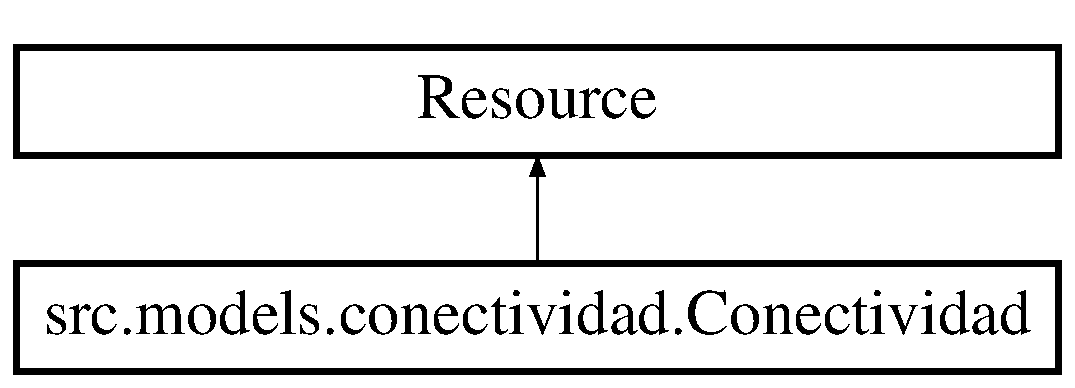
\includegraphics[height=2.000000cm]{classsrc_1_1models_1_1conectividad_1_1_conectividad}
\end{center}
\end{figure}
\subsection*{Métodos públicos}
\begin{DoxyCompactItemize}
\item 
\hypertarget{classsrc_1_1models_1_1conectividad_1_1_conectividad_ac32362e5db32d788fb1bb0bc21b36b6e}{def {\bfseries \-\_\-\-\_\-init\-\_\-\-\_\-}}\label{classsrc_1_1models_1_1conectividad_1_1_conectividad_ac32362e5db32d788fb1bb0bc21b36b6e}

\item 
def \hyperlink{classsrc_1_1models_1_1conectividad_1_1_conectividad_a1c6a08424c9406f4e47bfa4f8deb3bc6}{post}
\begin{DoxyCompactList}\small\item\em Permite realizar una peticion P\-O\-S\-T y obtener el json de respuesta o false si fallo. \end{DoxyCompactList}\item 
def \hyperlink{classsrc_1_1models_1_1conectividad_1_1_conectividad_ac0413d7dd62357ed0c3194a912eab085}{get}
\begin{DoxyCompactList}\small\item\em Permite realizar una peticion P\-O\-S\-T y obtener el json de respuesta o false si fallo. \end{DoxyCompactList}\item 
def \hyperlink{classsrc_1_1models_1_1conectividad_1_1_conectividad_ac093b5f0c19ff3fc5e5ee44eaf0fa54e}{put}
\begin{DoxyCompactList}\small\item\em Permite realizar una peticion P\-O\-S\-T y obtener el json de respuesta o false si fallo. \end{DoxyCompactList}\item 
def \hyperlink{classsrc_1_1models_1_1conectividad_1_1_conectividad_a9b9bbcb408c76c1c051633929d179be3}{delete}
\begin{DoxyCompactList}\small\item\em Permite realizar una peticion P\-O\-S\-T y obtener el json de respuesta o false si fallo. \end{DoxyCompactList}\item 
def \hyperlink{classsrc_1_1models_1_1conectividad_1_1_conectividad_aa728c32ed6b4dded19ce5d7b32638911}{renovar\-Token}
\begin{DoxyCompactList}\small\item\em Renueva el token si pasaron 5 horas. \end{DoxyCompactList}\end{DoxyCompactItemize}
\subsection*{Atributos públicos}
\begin{DoxyCompactItemize}
\item 
\hypertarget{classsrc_1_1models_1_1conectividad_1_1_conectividad_a97eb54522c4d907b516f86b1f252277a}{{\bfseries ultima\-Vez}}\label{classsrc_1_1models_1_1conectividad_1_1_conectividad_a97eb54522c4d907b516f86b1f252277a}

\item 
\hypertarget{classsrc_1_1models_1_1conectividad_1_1_conectividad_a87a6424e6c79858c600bf775c179f6cb}{{\bfseries app\-Server\-Token}}\label{classsrc_1_1models_1_1conectividad_1_1_conectividad_a87a6424e6c79858c600bf775c179f6cb}

\end{DoxyCompactItemize}


\subsection{Descripción detallada}
Clase para el manejo de las peticiones H\-T\-T\-P. 

Singleton. 

\subsection{Documentación de las funciones miembro}
\hypertarget{classsrc_1_1models_1_1conectividad_1_1_conectividad_a9b9bbcb408c76c1c051633929d179be3}{\index{src\-::models\-::conectividad\-::\-Conectividad@{src\-::models\-::conectividad\-::\-Conectividad}!delete@{delete}}
\index{delete@{delete}!src::models::conectividad::Conectividad@{src\-::models\-::conectividad\-::\-Conectividad}}
\subsubsection[{delete}]{\setlength{\rightskip}{0pt plus 5cm}def src.\-models.\-conectividad.\-Conectividad.\-delete (
\begin{DoxyParamCaption}
\item[{}]{self, }
\item[{}]{U\-R\-L, }
\item[{}]{endpoint, }
\item[{}]{diccionario\-Cuerpo = {\ttfamily \{\}}, }
\item[{}]{diccionario\-Parametros = {\ttfamily \{\}}}
\end{DoxyParamCaption}
)}}\label{classsrc_1_1models_1_1conectividad_1_1_conectividad_a9b9bbcb408c76c1c051633929d179be3}


Permite realizar una peticion P\-O\-S\-T y obtener el json de respuesta o false si fallo. 


\begin{DoxyParams}{Parámetros}
{\em endpoint} & El nombre del endpoint especifico sin la U\-R\-L base ni el caracter '/'. Ej\-: 'user'. \\
\hline
{\em diccionario\-Cuerpo} & Los pares clave-\/valor (en forma de diccionario) a enviar en el cuerpo de la peticion. \\
\hline
{\em diccionario\-Parametros} & Los pares clave-\/valor (en forma de diccionario) a enviar como parametros de la peticion. \\
\hline
\end{DoxyParams}
\hypertarget{classsrc_1_1models_1_1conectividad_1_1_conectividad_ac0413d7dd62357ed0c3194a912eab085}{\index{src\-::models\-::conectividad\-::\-Conectividad@{src\-::models\-::conectividad\-::\-Conectividad}!get@{get}}
\index{get@{get}!src::models::conectividad::Conectividad@{src\-::models\-::conectividad\-::\-Conectividad}}
\subsubsection[{get}]{\setlength{\rightskip}{0pt plus 5cm}def src.\-models.\-conectividad.\-Conectividad.\-get (
\begin{DoxyParamCaption}
\item[{}]{self, }
\item[{}]{U\-R\-L, }
\item[{}]{endpoint, }
\item[{}]{diccionario\-Parametros = {\ttfamily \{\}}}
\end{DoxyParamCaption}
)}}\label{classsrc_1_1models_1_1conectividad_1_1_conectividad_ac0413d7dd62357ed0c3194a912eab085}


Permite realizar una peticion P\-O\-S\-T y obtener el json de respuesta o false si fallo. 


\begin{DoxyParams}{Parámetros}
{\em endpoint} & El nombre del endpoint especifico sin la U\-R\-L base ni el caracter '/'. Ej\-: 'user'. \\
\hline
{\em diccionario\-Parametros} & Los pares clave-\/valor (en forma de diccionario) a enviar como parametros de la peticion. \\
\hline
\end{DoxyParams}
\hypertarget{classsrc_1_1models_1_1conectividad_1_1_conectividad_a1c6a08424c9406f4e47bfa4f8deb3bc6}{\index{src\-::models\-::conectividad\-::\-Conectividad@{src\-::models\-::conectividad\-::\-Conectividad}!post@{post}}
\index{post@{post}!src::models::conectividad::Conectividad@{src\-::models\-::conectividad\-::\-Conectividad}}
\subsubsection[{post}]{\setlength{\rightskip}{0pt plus 5cm}def src.\-models.\-conectividad.\-Conectividad.\-post (
\begin{DoxyParamCaption}
\item[{}]{self, }
\item[{}]{U\-R\-L, }
\item[{}]{endpoint, }
\item[{}]{diccionario\-Cuerpo = {\ttfamily \{\}}, }
\item[{}]{diccionario\-Parametros = {\ttfamily \{\}}, }
\item[{}]{diccionario\-Header = {\ttfamily \{\}}}
\end{DoxyParamCaption}
)}}\label{classsrc_1_1models_1_1conectividad_1_1_conectividad_a1c6a08424c9406f4e47bfa4f8deb3bc6}


Permite realizar una peticion P\-O\-S\-T y obtener el json de respuesta o false si fallo. 


\begin{DoxyParams}{Parámetros}
{\em endpoint} & El nombre del endpoint especifico sin la U\-R\-L base ni el caracter '/'. Ej\-: 'user'. \\
\hline
{\em diccionario\-Cuerpo} & Los pares clave-\/valor (en forma de diccionario) a enviar en el cuerpo de la peticion. \\
\hline
{\em diccionario\-Parametros} & Los pares clave-\/valor (en forma de diccionario) a enviar como parametros de la peticion. \\
\hline
\end{DoxyParams}
\hypertarget{classsrc_1_1models_1_1conectividad_1_1_conectividad_ac093b5f0c19ff3fc5e5ee44eaf0fa54e}{\index{src\-::models\-::conectividad\-::\-Conectividad@{src\-::models\-::conectividad\-::\-Conectividad}!put@{put}}
\index{put@{put}!src::models::conectividad::Conectividad@{src\-::models\-::conectividad\-::\-Conectividad}}
\subsubsection[{put}]{\setlength{\rightskip}{0pt plus 5cm}def src.\-models.\-conectividad.\-Conectividad.\-put (
\begin{DoxyParamCaption}
\item[{}]{self, }
\item[{}]{U\-R\-L, }
\item[{}]{endpoint, }
\item[{}]{diccionario\-Cuerpo = {\ttfamily \{\}}, }
\item[{}]{diccionario\-Parametros = {\ttfamily \{\}}}
\end{DoxyParamCaption}
)}}\label{classsrc_1_1models_1_1conectividad_1_1_conectividad_ac093b5f0c19ff3fc5e5ee44eaf0fa54e}


Permite realizar una peticion P\-O\-S\-T y obtener el json de respuesta o false si fallo. 


\begin{DoxyParams}{Parámetros}
{\em endpoint} & El nombre del endpoint especifico sin la U\-R\-L base ni el caracter '/'. Ej\-: 'user'. \\
\hline
{\em diccionario\-Cuerpo} & Los pares clave-\/valor (en forma de diccionario) a enviar en el cuerpo de la peticion. \\
\hline
{\em diccionario\-Parametros} & Los pares clave-\/valor (en forma de diccionario) a enviar como parametros de la peticion. \\
\hline
\end{DoxyParams}
\hypertarget{classsrc_1_1models_1_1conectividad_1_1_conectividad_aa728c32ed6b4dded19ce5d7b32638911}{\index{src\-::models\-::conectividad\-::\-Conectividad@{src\-::models\-::conectividad\-::\-Conectividad}!renovar\-Token@{renovar\-Token}}
\index{renovar\-Token@{renovar\-Token}!src::models::conectividad::Conectividad@{src\-::models\-::conectividad\-::\-Conectividad}}
\subsubsection[{renovar\-Token}]{\setlength{\rightskip}{0pt plus 5cm}def src.\-models.\-conectividad.\-Conectividad.\-renovar\-Token (
\begin{DoxyParamCaption}
\item[{}]{self}
\end{DoxyParamCaption}
)}}\label{classsrc_1_1models_1_1conectividad_1_1_conectividad_aa728c32ed6b4dded19ce5d7b32638911}


Renueva el token si pasaron 5 horas. 



La documentación para esta clase fue generada a partir del siguiente fichero\-:\begin{DoxyCompactItemize}
\item 
src/models/conectividad.\-py\end{DoxyCompactItemize}

\hypertarget{classsrc_1_1resources_1_1eliminar_auto_usuario_1_1_eliminar_auto_usuario}{\section{Referencia de la Clase src.\-resources.\-eliminar\-Auto\-Usuario.\-Eliminar\-Auto\-Usuario}
\label{classsrc_1_1resources_1_1eliminar_auto_usuario_1_1_eliminar_auto_usuario}\index{src.\-resources.\-eliminar\-Auto\-Usuario.\-Eliminar\-Auto\-Usuario@{src.\-resources.\-eliminar\-Auto\-Usuario.\-Eliminar\-Auto\-Usuario}}
}


Clase para eliminar un auto de un usuario.  


Diagrama de herencias de src.\-resources.\-eliminar\-Auto\-Usuario.\-Eliminar\-Auto\-Usuario\begin{figure}[H]
\begin{center}
\leavevmode
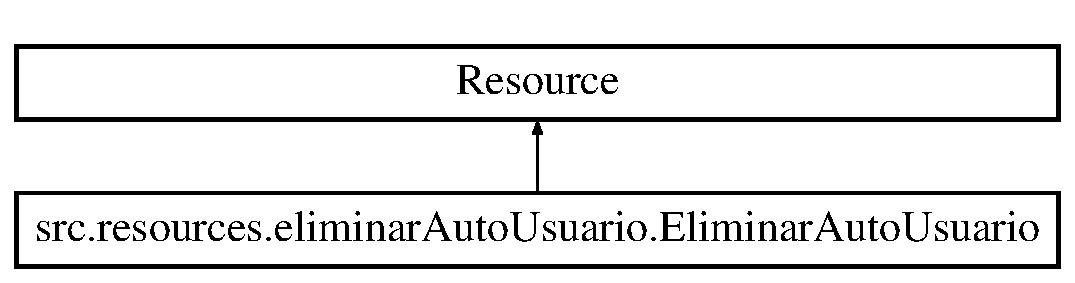
\includegraphics[height=2.000000cm]{classsrc_1_1resources_1_1eliminar_auto_usuario_1_1_eliminar_auto_usuario}
\end{center}
\end{figure}
\subsection*{Métodos públicos}
\begin{DoxyCompactItemize}
\item 
\hypertarget{classsrc_1_1resources_1_1eliminar_auto_usuario_1_1_eliminar_auto_usuario_aabebf5d292e7ee2ed564aada86f1dc95}{def {\bfseries \-\_\-\-\_\-init\-\_\-\-\_\-}}\label{classsrc_1_1resources_1_1eliminar_auto_usuario_1_1_eliminar_auto_usuario_aabebf5d292e7ee2ed564aada86f1dc95}

\item 
def \hyperlink{classsrc_1_1resources_1_1eliminar_auto_usuario_1_1_eliminar_auto_usuario_aac1268a9c74bab80d45a5a38fe618373}{delete}
\begin{DoxyCompactList}\small\item\em Elimina un auto de un usuario determinado. \end{DoxyCompactList}\end{DoxyCompactItemize}
\subsection*{Atributos públicos}
\begin{DoxyCompactItemize}
\item 
\hypertarget{classsrc_1_1resources_1_1eliminar_auto_usuario_1_1_eliminar_auto_usuario_ab77bd6a65a9a217084342983fed700d3}{{\bfseries autenticador}}\label{classsrc_1_1resources_1_1eliminar_auto_usuario_1_1_eliminar_auto_usuario_ab77bd6a65a9a217084342983fed700d3}

\end{DoxyCompactItemize}
\subsection*{Métodos privados}
\begin{DoxyCompactItemize}
\item 
def \hyperlink{classsrc_1_1resources_1_1eliminar_auto_usuario_1_1_eliminar_auto_usuario_aab03bbccdc074042c069401e1f2c6a84}{\-\_\-validar\-\_\-token}
\begin{DoxyCompactList}\small\item\em Valida al usuario. \end{DoxyCompactList}\end{DoxyCompactItemize}


\subsection{Descripción detallada}
Clase para eliminar un auto de un usuario. 



\subsection{Documentación de las funciones miembro}
\hypertarget{classsrc_1_1resources_1_1eliminar_auto_usuario_1_1_eliminar_auto_usuario_aab03bbccdc074042c069401e1f2c6a84}{\index{src\-::resources\-::eliminar\-Auto\-Usuario\-::\-Eliminar\-Auto\-Usuario@{src\-::resources\-::eliminar\-Auto\-Usuario\-::\-Eliminar\-Auto\-Usuario}!\-\_\-validar\-\_\-token@{\-\_\-validar\-\_\-token}}
\index{\-\_\-validar\-\_\-token@{\-\_\-validar\-\_\-token}!src::resources::eliminarAutoUsuario::EliminarAutoUsuario@{src\-::resources\-::eliminar\-Auto\-Usuario\-::\-Eliminar\-Auto\-Usuario}}
\subsubsection[{\-\_\-validar\-\_\-token}]{\setlength{\rightskip}{0pt plus 5cm}def src.\-resources.\-eliminar\-Auto\-Usuario.\-Eliminar\-Auto\-Usuario.\-\_\-validar\-\_\-token (
\begin{DoxyParamCaption}
\item[{}]{self}
\end{DoxyParamCaption}
)\hspace{0.3cm}{\ttfamily [private]}}}\label{classsrc_1_1resources_1_1eliminar_auto_usuario_1_1_eliminar_auto_usuario_aab03bbccdc074042c069401e1f2c6a84}


Valida al usuario. 

\hypertarget{classsrc_1_1resources_1_1eliminar_auto_usuario_1_1_eliminar_auto_usuario_aac1268a9c74bab80d45a5a38fe618373}{\index{src\-::resources\-::eliminar\-Auto\-Usuario\-::\-Eliminar\-Auto\-Usuario@{src\-::resources\-::eliminar\-Auto\-Usuario\-::\-Eliminar\-Auto\-Usuario}!delete@{delete}}
\index{delete@{delete}!src::resources::eliminarAutoUsuario::EliminarAutoUsuario@{src\-::resources\-::eliminar\-Auto\-Usuario\-::\-Eliminar\-Auto\-Usuario}}
\subsubsection[{delete}]{\setlength{\rightskip}{0pt plus 5cm}def src.\-resources.\-eliminar\-Auto\-Usuario.\-Eliminar\-Auto\-Usuario.\-delete (
\begin{DoxyParamCaption}
\item[{}]{self, }
\item[{}]{I\-D\-Usuario, }
\item[{}]{I\-D\-Auto}
\end{DoxyParamCaption}
)}}\label{classsrc_1_1resources_1_1eliminar_auto_usuario_1_1_eliminar_auto_usuario_aac1268a9c74bab80d45a5a38fe618373}


Elimina un auto de un usuario determinado. 



La documentación para esta clase fue generada a partir del siguiente fichero\-:\begin{DoxyCompactItemize}
\item 
src/resources/eliminar\-Auto\-Usuario.\-py\end{DoxyCompactItemize}

\hypertarget{classsrc_1_1resources_1_1error__handler_1_1_error_handler}{\section{Referencia de la Clase src.\-resources.\-error\-\_\-handler.\-Error\-Handler}
\label{classsrc_1_1resources_1_1error__handler_1_1_error_handler}\index{src.\-resources.\-error\-\_\-handler.\-Error\-Handler@{src.\-resources.\-error\-\_\-handler.\-Error\-Handler}}
}


Clase para creacion de errores.  


\subsection*{Métodos públicos estáticos}
\begin{DoxyCompactItemize}
\item 
\hypertarget{classsrc_1_1resources_1_1error__handler_1_1_error_handler_a93f481928c27dccb20a627eaa35f6224}{def \hyperlink{classsrc_1_1resources_1_1error__handler_1_1_error_handler_a93f481928c27dccb20a627eaa35f6224}{create\-\_\-error\-\_\-response}}\label{classsrc_1_1resources_1_1error__handler_1_1_error_handler_a93f481928c27dccb20a627eaa35f6224}

\begin{DoxyCompactList}\small\item\em Crea un Json con el codigo y el mensaje de error. \end{DoxyCompactList}\end{DoxyCompactItemize}


\subsection{Descripción detallada}
Clase para creacion de errores. 

Para ver creacion de respuestas correctas\-: \hyperlink{classsrc_1_1resources_1_1response__builder_1_1_response_builder}{response\-\_\-builder.\-Response\-Builder} 

La documentación para esta clase fue generada a partir del siguiente fichero\-:\begin{DoxyCompactItemize}
\item 
src/resources/error\-\_\-handler.\-py\end{DoxyCompactItemize}

\hypertarget{classsrc_1_1resources_1_1index_1_1_hello_world}{\section{Referencia de la Clase src.\-resources.\-index.\-Hello\-World}
\label{classsrc_1_1resources_1_1index_1_1_hello_world}\index{src.\-resources.\-index.\-Hello\-World@{src.\-resources.\-index.\-Hello\-World}}
}


Inicializa la vista del App\-Server.  


Diagrama de herencias de src.\-resources.\-index.\-Hello\-World\begin{figure}[H]
\begin{center}
\leavevmode
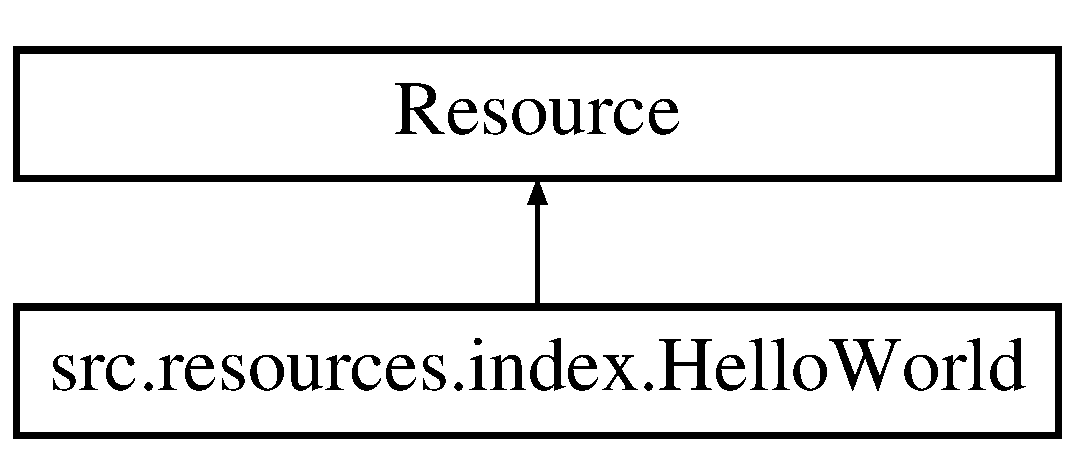
\includegraphics[height=2.000000cm]{classsrc_1_1resources_1_1index_1_1_hello_world}
\end{center}
\end{figure}
\subsection*{Métodos públicos}
\begin{DoxyCompactItemize}
\item 
\hypertarget{classsrc_1_1resources_1_1index_1_1_hello_world_a35cae5cb28b3d64bf1e74089fc6b2930}{def {\bfseries get}}\label{classsrc_1_1resources_1_1index_1_1_hello_world_a35cae5cb28b3d64bf1e74089fc6b2930}

\end{DoxyCompactItemize}


\subsection{Descripción detallada}
Inicializa la vista del App\-Server. 

La documentación para esta clase fue generada a partir del siguiente fichero\-:\begin{DoxyCompactItemize}
\item 
src/resources/index.\-py\end{DoxyCompactItemize}

\hypertarget{classsrc_1_1resources_1_1modificar_auto_usuario_1_1_modificar_auto_usuario}{\section{Referencia de la Clase src.\-resources.\-modificar\-Auto\-Usuario.\-Modificar\-Auto\-Usuario}
\label{classsrc_1_1resources_1_1modificar_auto_usuario_1_1_modificar_auto_usuario}\index{src.\-resources.\-modificar\-Auto\-Usuario.\-Modificar\-Auto\-Usuario@{src.\-resources.\-modificar\-Auto\-Usuario.\-Modificar\-Auto\-Usuario}}
}


Clase para modificar un auto de un usuario.  


Diagrama de herencias de src.\-resources.\-modificar\-Auto\-Usuario.\-Modificar\-Auto\-Usuario\begin{figure}[H]
\begin{center}
\leavevmode
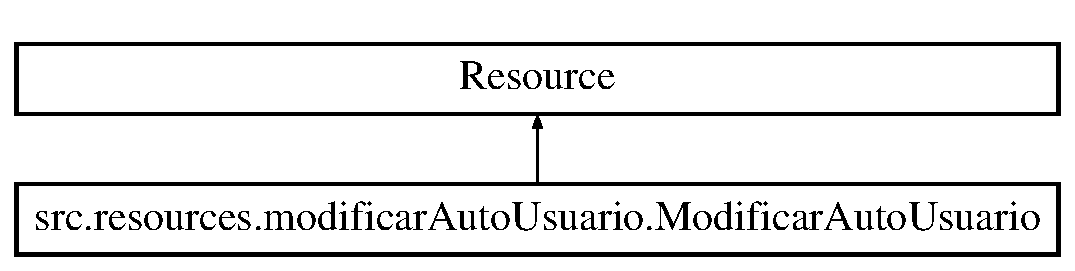
\includegraphics[height=2.000000cm]{classsrc_1_1resources_1_1modificar_auto_usuario_1_1_modificar_auto_usuario}
\end{center}
\end{figure}
\subsection*{Métodos públicos}
\begin{DoxyCompactItemize}
\item 
\hypertarget{classsrc_1_1resources_1_1modificar_auto_usuario_1_1_modificar_auto_usuario_a61c9a0026e46c161bf9b09dff39eb675}{def {\bfseries \-\_\-\-\_\-init\-\_\-\-\_\-}}\label{classsrc_1_1resources_1_1modificar_auto_usuario_1_1_modificar_auto_usuario_a61c9a0026e46c161bf9b09dff39eb675}

\item 
def \hyperlink{classsrc_1_1resources_1_1modificar_auto_usuario_1_1_modificar_auto_usuario_a600fa25d061c4fd53659bb3afea11c4a}{put}
\begin{DoxyCompactList}\small\item\em Modifica los datos de un auto de un determinado usuario. \end{DoxyCompactList}\end{DoxyCompactItemize}
\subsection*{Atributos públicos}
\begin{DoxyCompactItemize}
\item 
\hypertarget{classsrc_1_1resources_1_1modificar_auto_usuario_1_1_modificar_auto_usuario_a412b33ba625ecce071da19cad1ed3a5c}{{\bfseries autenticador}}\label{classsrc_1_1resources_1_1modificar_auto_usuario_1_1_modificar_auto_usuario_a412b33ba625ecce071da19cad1ed3a5c}

\end{DoxyCompactItemize}
\subsection*{Métodos privados}
\begin{DoxyCompactItemize}
\item 
def \hyperlink{classsrc_1_1resources_1_1modificar_auto_usuario_1_1_modificar_auto_usuario_a841232f86697888e9a4b529da2091673}{\-\_\-get\-\_\-data\-\_\-from\-\_\-request}
\begin{DoxyCompactList}\small\item\em Obtiene la propiedad del json contenido de la request. \end{DoxyCompactList}\item 
def \hyperlink{classsrc_1_1resources_1_1modificar_auto_usuario_1_1_modificar_auto_usuario_a50d718aa494a3c60a6c50541229a91c1}{\-\_\-validate\-\_\-request}
\begin{DoxyCompactList}\small\item\em Valida que haya una request completa. \end{DoxyCompactList}\item 
def \hyperlink{classsrc_1_1resources_1_1modificar_auto_usuario_1_1_modificar_auto_usuario_a4542c80a3b2eb14aff8eeeb88bb2d16d}{\-\_\-validar\-\_\-token}
\begin{DoxyCompactList}\small\item\em Valida al usuario. \end{DoxyCompactList}\item 
\hypertarget{classsrc_1_1resources_1_1modificar_auto_usuario_1_1_modificar_auto_usuario_a6a30c8d70789c069be09af71bbb75fe4}{def {\bfseries \-\_\-obtener\-J\-S\-O\-N\-Propiedades\-Auto}}\label{classsrc_1_1resources_1_1modificar_auto_usuario_1_1_modificar_auto_usuario_a6a30c8d70789c069be09af71bbb75fe4}

\item 
\hypertarget{classsrc_1_1resources_1_1modificar_auto_usuario_1_1_modificar_auto_usuario_a6e67b5caca1524c720f80ce3b176fba3}{def {\bfseries \-\_\-obtener\-J\-S\-O\-N}}\label{classsrc_1_1resources_1_1modificar_auto_usuario_1_1_modificar_auto_usuario_a6e67b5caca1524c720f80ce3b176fba3}

\end{DoxyCompactItemize}


\subsection{Descripción detallada}
Clase para modificar un auto de un usuario. 



\subsection{Documentación de las funciones miembro}
\hypertarget{classsrc_1_1resources_1_1modificar_auto_usuario_1_1_modificar_auto_usuario_a841232f86697888e9a4b529da2091673}{\index{src\-::resources\-::modificar\-Auto\-Usuario\-::\-Modificar\-Auto\-Usuario@{src\-::resources\-::modificar\-Auto\-Usuario\-::\-Modificar\-Auto\-Usuario}!\-\_\-get\-\_\-data\-\_\-from\-\_\-request@{\-\_\-get\-\_\-data\-\_\-from\-\_\-request}}
\index{\-\_\-get\-\_\-data\-\_\-from\-\_\-request@{\-\_\-get\-\_\-data\-\_\-from\-\_\-request}!src::resources::modificarAutoUsuario::ModificarAutoUsuario@{src\-::resources\-::modificar\-Auto\-Usuario\-::\-Modificar\-Auto\-Usuario}}
\subsubsection[{\-\_\-get\-\_\-data\-\_\-from\-\_\-request}]{\setlength{\rightskip}{0pt plus 5cm}def src.\-resources.\-modificar\-Auto\-Usuario.\-Modificar\-Auto\-Usuario.\-\_\-get\-\_\-data\-\_\-from\-\_\-request (
\begin{DoxyParamCaption}
\item[{}]{self, }
\item[{}]{nombre\-Propiedad, }
\item[{}]{defecto = {\ttfamily False}}
\end{DoxyParamCaption}
)\hspace{0.3cm}{\ttfamily [private]}}}\label{classsrc_1_1resources_1_1modificar_auto_usuario_1_1_modificar_auto_usuario_a841232f86697888e9a4b529da2091673}


Obtiene la propiedad del json contenido de la request. 

\hypertarget{classsrc_1_1resources_1_1modificar_auto_usuario_1_1_modificar_auto_usuario_a4542c80a3b2eb14aff8eeeb88bb2d16d}{\index{src\-::resources\-::modificar\-Auto\-Usuario\-::\-Modificar\-Auto\-Usuario@{src\-::resources\-::modificar\-Auto\-Usuario\-::\-Modificar\-Auto\-Usuario}!\-\_\-validar\-\_\-token@{\-\_\-validar\-\_\-token}}
\index{\-\_\-validar\-\_\-token@{\-\_\-validar\-\_\-token}!src::resources::modificarAutoUsuario::ModificarAutoUsuario@{src\-::resources\-::modificar\-Auto\-Usuario\-::\-Modificar\-Auto\-Usuario}}
\subsubsection[{\-\_\-validar\-\_\-token}]{\setlength{\rightskip}{0pt plus 5cm}def src.\-resources.\-modificar\-Auto\-Usuario.\-Modificar\-Auto\-Usuario.\-\_\-validar\-\_\-token (
\begin{DoxyParamCaption}
\item[{}]{self}
\end{DoxyParamCaption}
)\hspace{0.3cm}{\ttfamily [private]}}}\label{classsrc_1_1resources_1_1modificar_auto_usuario_1_1_modificar_auto_usuario_a4542c80a3b2eb14aff8eeeb88bb2d16d}


Valida al usuario. 

\hypertarget{classsrc_1_1resources_1_1modificar_auto_usuario_1_1_modificar_auto_usuario_a50d718aa494a3c60a6c50541229a91c1}{\index{src\-::resources\-::modificar\-Auto\-Usuario\-::\-Modificar\-Auto\-Usuario@{src\-::resources\-::modificar\-Auto\-Usuario\-::\-Modificar\-Auto\-Usuario}!\-\_\-validate\-\_\-request@{\-\_\-validate\-\_\-request}}
\index{\-\_\-validate\-\_\-request@{\-\_\-validate\-\_\-request}!src::resources::modificarAutoUsuario::ModificarAutoUsuario@{src\-::resources\-::modificar\-Auto\-Usuario\-::\-Modificar\-Auto\-Usuario}}
\subsubsection[{\-\_\-validate\-\_\-request}]{\setlength{\rightskip}{0pt plus 5cm}def src.\-resources.\-modificar\-Auto\-Usuario.\-Modificar\-Auto\-Usuario.\-\_\-validate\-\_\-request (
\begin{DoxyParamCaption}
\item[{}]{self}
\end{DoxyParamCaption}
)\hspace{0.3cm}{\ttfamily [private]}}}\label{classsrc_1_1resources_1_1modificar_auto_usuario_1_1_modificar_auto_usuario_a50d718aa494a3c60a6c50541229a91c1}


Valida que haya una request completa. 

\hypertarget{classsrc_1_1resources_1_1modificar_auto_usuario_1_1_modificar_auto_usuario_a600fa25d061c4fd53659bb3afea11c4a}{\index{src\-::resources\-::modificar\-Auto\-Usuario\-::\-Modificar\-Auto\-Usuario@{src\-::resources\-::modificar\-Auto\-Usuario\-::\-Modificar\-Auto\-Usuario}!put@{put}}
\index{put@{put}!src::resources::modificarAutoUsuario::ModificarAutoUsuario@{src\-::resources\-::modificar\-Auto\-Usuario\-::\-Modificar\-Auto\-Usuario}}
\subsubsection[{put}]{\setlength{\rightskip}{0pt plus 5cm}def src.\-resources.\-modificar\-Auto\-Usuario.\-Modificar\-Auto\-Usuario.\-put (
\begin{DoxyParamCaption}
\item[{}]{self, }
\item[{}]{I\-D\-Usuario, }
\item[{}]{I\-D\-Auto, }
\item[{}]{ref}
\end{DoxyParamCaption}
)}}\label{classsrc_1_1resources_1_1modificar_auto_usuario_1_1_modificar_auto_usuario_a600fa25d061c4fd53659bb3afea11c4a}


Modifica los datos de un auto de un determinado usuario. 



La documentación para esta clase fue generada a partir del siguiente fichero\-:\begin{DoxyCompactItemize}
\item 
src/resources/modificar\-Auto\-Usuario.\-py\end{DoxyCompactItemize}

\hypertarget{classsrc_1_1resources_1_1obtener_posibles_viajes_1_1_obtener_posibles_viajes}{\section{Referencia de la Clase src.\-resources.\-obtener\-Posibles\-Viajes.\-Obtener\-Posibles\-Viajes}
\label{classsrc_1_1resources_1_1obtener_posibles_viajes_1_1_obtener_posibles_viajes}\index{src.\-resources.\-obtener\-Posibles\-Viajes.\-Obtener\-Posibles\-Viajes@{src.\-resources.\-obtener\-Posibles\-Viajes.\-Obtener\-Posibles\-Viajes}}
}


Clase para obtener la lista de posibles viajes de un chofer.  


Diagrama de herencias de src.\-resources.\-obtener\-Posibles\-Viajes.\-Obtener\-Posibles\-Viajes\begin{figure}[H]
\begin{center}
\leavevmode
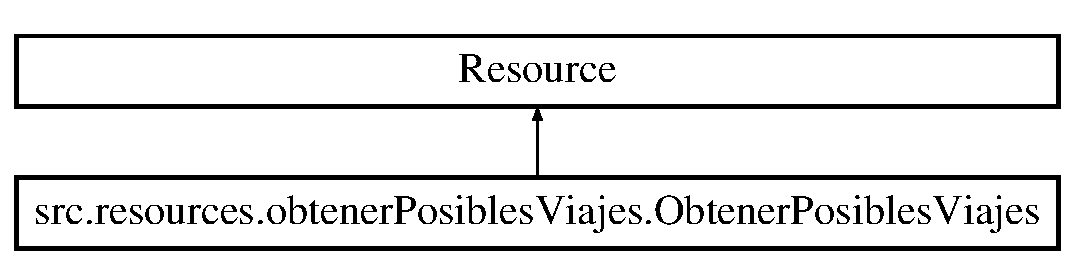
\includegraphics[height=2.000000cm]{classsrc_1_1resources_1_1obtener_posibles_viajes_1_1_obtener_posibles_viajes}
\end{center}
\end{figure}
\subsection*{Métodos públicos}
\begin{DoxyCompactItemize}
\item 
\hypertarget{classsrc_1_1resources_1_1obtener_posibles_viajes_1_1_obtener_posibles_viajes_ad93d3f991ef591efe6c5cef717b75967}{def {\bfseries \-\_\-\-\_\-init\-\_\-\-\_\-}}\label{classsrc_1_1resources_1_1obtener_posibles_viajes_1_1_obtener_posibles_viajes_ad93d3f991ef591efe6c5cef717b75967}

\item 
def \hyperlink{classsrc_1_1resources_1_1obtener_posibles_viajes_1_1_obtener_posibles_viajes_a987e5ab35e776e08efdd48277fc0f139}{get}
\begin{DoxyCompactList}\small\item\em Obtiene la informacion de todos los viajes posibles. \end{DoxyCompactList}\end{DoxyCompactItemize}
\subsection*{Atributos públicos}
\begin{DoxyCompactItemize}
\item 
\hypertarget{classsrc_1_1resources_1_1obtener_posibles_viajes_1_1_obtener_posibles_viajes_ab67410503478154e68e81ce1b95516b2}{{\bfseries autenticador}}\label{classsrc_1_1resources_1_1obtener_posibles_viajes_1_1_obtener_posibles_viajes_ab67410503478154e68e81ce1b95516b2}

\end{DoxyCompactItemize}
\subsection*{Métodos privados}
\begin{DoxyCompactItemize}
\item 
def \hyperlink{classsrc_1_1resources_1_1obtener_posibles_viajes_1_1_obtener_posibles_viajes_a7f4c696de51b7e99028c851b5b25648f}{\-\_\-validar\-\_\-token}
\begin{DoxyCompactList}\small\item\em Valida al usuario. \end{DoxyCompactList}\item 
def \hyperlink{classsrc_1_1resources_1_1obtener_posibles_viajes_1_1_obtener_posibles_viajes_abf3d98b7d87231a0fee98474aa94261f}{\-\_\-obtener\-J\-S\-O\-N\-Viajes}
\begin{DoxyCompactList}\small\item\em Obtiene toda la informacion y crea el J\-S\-O\-N de datos del viajes. \end{DoxyCompactList}\end{DoxyCompactItemize}


\subsection{Descripción detallada}
Clase para obtener la lista de posibles viajes de un chofer. 



\subsection{Documentación de las funciones miembro}
\hypertarget{classsrc_1_1resources_1_1obtener_posibles_viajes_1_1_obtener_posibles_viajes_abf3d98b7d87231a0fee98474aa94261f}{\index{src\-::resources\-::obtener\-Posibles\-Viajes\-::\-Obtener\-Posibles\-Viajes@{src\-::resources\-::obtener\-Posibles\-Viajes\-::\-Obtener\-Posibles\-Viajes}!\-\_\-obtener\-J\-S\-O\-N\-Viajes@{\-\_\-obtener\-J\-S\-O\-N\-Viajes}}
\index{\-\_\-obtener\-J\-S\-O\-N\-Viajes@{\-\_\-obtener\-J\-S\-O\-N\-Viajes}!src::resources::obtenerPosiblesViajes::ObtenerPosiblesViajes@{src\-::resources\-::obtener\-Posibles\-Viajes\-::\-Obtener\-Posibles\-Viajes}}
\subsubsection[{\-\_\-obtener\-J\-S\-O\-N\-Viajes}]{\setlength{\rightskip}{0pt plus 5cm}def src.\-resources.\-obtener\-Posibles\-Viajes.\-Obtener\-Posibles\-Viajes.\-\_\-obtener\-J\-S\-O\-N\-Viajes (
\begin{DoxyParamCaption}
\item[{}]{self, }
\item[{}]{I\-D\-Usuario}
\end{DoxyParamCaption}
)\hspace{0.3cm}{\ttfamily [private]}}}\label{classsrc_1_1resources_1_1obtener_posibles_viajes_1_1_obtener_posibles_viajes_abf3d98b7d87231a0fee98474aa94261f}


Obtiene toda la informacion y crea el J\-S\-O\-N de datos del viajes. 

\hypertarget{classsrc_1_1resources_1_1obtener_posibles_viajes_1_1_obtener_posibles_viajes_a7f4c696de51b7e99028c851b5b25648f}{\index{src\-::resources\-::obtener\-Posibles\-Viajes\-::\-Obtener\-Posibles\-Viajes@{src\-::resources\-::obtener\-Posibles\-Viajes\-::\-Obtener\-Posibles\-Viajes}!\-\_\-validar\-\_\-token@{\-\_\-validar\-\_\-token}}
\index{\-\_\-validar\-\_\-token@{\-\_\-validar\-\_\-token}!src::resources::obtenerPosiblesViajes::ObtenerPosiblesViajes@{src\-::resources\-::obtener\-Posibles\-Viajes\-::\-Obtener\-Posibles\-Viajes}}
\subsubsection[{\-\_\-validar\-\_\-token}]{\setlength{\rightskip}{0pt plus 5cm}def src.\-resources.\-obtener\-Posibles\-Viajes.\-Obtener\-Posibles\-Viajes.\-\_\-validar\-\_\-token (
\begin{DoxyParamCaption}
\item[{}]{self}
\end{DoxyParamCaption}
)\hspace{0.3cm}{\ttfamily [private]}}}\label{classsrc_1_1resources_1_1obtener_posibles_viajes_1_1_obtener_posibles_viajes_a7f4c696de51b7e99028c851b5b25648f}


Valida al usuario. 

\hypertarget{classsrc_1_1resources_1_1obtener_posibles_viajes_1_1_obtener_posibles_viajes_a987e5ab35e776e08efdd48277fc0f139}{\index{src\-::resources\-::obtener\-Posibles\-Viajes\-::\-Obtener\-Posibles\-Viajes@{src\-::resources\-::obtener\-Posibles\-Viajes\-::\-Obtener\-Posibles\-Viajes}!get@{get}}
\index{get@{get}!src::resources::obtenerPosiblesViajes::ObtenerPosiblesViajes@{src\-::resources\-::obtener\-Posibles\-Viajes\-::\-Obtener\-Posibles\-Viajes}}
\subsubsection[{get}]{\setlength{\rightskip}{0pt plus 5cm}def src.\-resources.\-obtener\-Posibles\-Viajes.\-Obtener\-Posibles\-Viajes.\-get (
\begin{DoxyParamCaption}
\item[{}]{self, }
\item[{}]{I\-D\-Usuario}
\end{DoxyParamCaption}
)}}\label{classsrc_1_1resources_1_1obtener_posibles_viajes_1_1_obtener_posibles_viajes_a987e5ab35e776e08efdd48277fc0f139}


Obtiene la informacion de todos los viajes posibles. 



La documentación para esta clase fue generada a partir del siguiente fichero\-:\begin{DoxyCompactItemize}
\item 
src/resources/obtener\-Posibles\-Viajes.\-py\end{DoxyCompactItemize}

\hypertarget{classsrc_1_1resources_1_1user_control_1_1_register}{\section{Referencia de la Clase src.\-resources.\-user\-Control.\-Register}
\label{classsrc_1_1resources_1_1user_control_1_1_register}\index{src.\-resources.\-user\-Control.\-Register@{src.\-resources.\-user\-Control.\-Register}}
}


Clase para registro de nuevo usuario.  


Diagrama de herencias de src.\-resources.\-user\-Control.\-Register\begin{figure}[H]
\begin{center}
\leavevmode
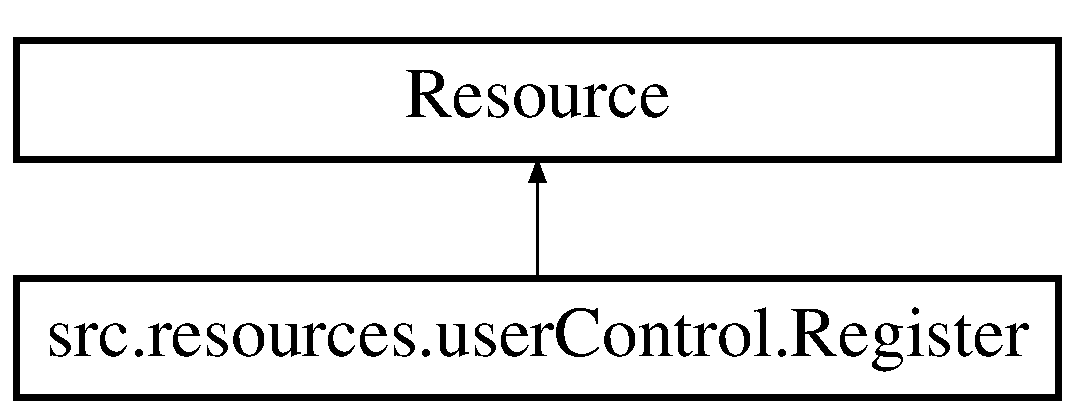
\includegraphics[height=2.000000cm]{classsrc_1_1resources_1_1user_control_1_1_register}
\end{center}
\end{figure}
\subsection*{Métodos públicos}
\begin{DoxyCompactItemize}
\item 
\hypertarget{classsrc_1_1resources_1_1user_control_1_1_register_ab0152d9e570205ce75980bac6f7ced78}{def {\bfseries get}}\label{classsrc_1_1resources_1_1user_control_1_1_register_ab0152d9e570205ce75980bac6f7ced78}

\item 
\hypertarget{classsrc_1_1resources_1_1user_control_1_1_register_a0cb2055635160abfce69a9d8ce1f44a1}{def \hyperlink{classsrc_1_1resources_1_1user_control_1_1_register_a0cb2055635160abfce69a9d8ce1f44a1}{post}}\label{classsrc_1_1resources_1_1user_control_1_1_register_a0cb2055635160abfce69a9d8ce1f44a1}

\begin{DoxyCompactList}\small\item\em Post\-: agrega un usuario. \end{DoxyCompactList}\end{DoxyCompactItemize}


\subsection{Descripción detallada}
Clase para registro de nuevo usuario. 

La documentación para esta clase fue generada a partir del siguiente fichero\-:\begin{DoxyCompactItemize}
\item 
src/resources/user\-Control.\-py\end{DoxyCompactItemize}

\hypertarget{classsrc_1_1resources_1_1response__builder_1_1_response_builder}{\section{Referencia de la Clase src.\-resources.\-response\-\_\-builder.\-Response\-Builder}
\label{classsrc_1_1resources_1_1response__builder_1_1_response_builder}\index{src.\-resources.\-response\-\_\-builder.\-Response\-Builder@{src.\-resources.\-response\-\_\-builder.\-Response\-Builder}}
}


Clase para creacion de responses.  


\subsection*{Métodos públicos estáticos}
\begin{DoxyCompactItemize}
\item 
\hypertarget{classsrc_1_1resources_1_1response__builder_1_1_response_builder_ac0c9842fd66095442c5f60f868d5c69b}{def \hyperlink{classsrc_1_1resources_1_1response__builder_1_1_response_builder_ac0c9842fd66095442c5f60f868d5c69b}{build\-\_\-response}}\label{classsrc_1_1resources_1_1response__builder_1_1_response_builder_ac0c9842fd66095442c5f60f868d5c69b}

\begin{DoxyCompactList}\small\item\em Crea un Json con la respuesta. \end{DoxyCompactList}\end{DoxyCompactItemize}


\subsection{Descripción detallada}
Clase para creacion de responses. 

Para ver creacion de errores\-: \hyperlink{classsrc_1_1resources_1_1error__handler_1_1_error_handler}{error\-\_\-handler.\-Error\-Handler} 

La documentación para esta clase fue generada a partir del siguiente fichero\-:\begin{DoxyCompactItemize}
\item 
src/resources/response\-\_\-builder.\-py\end{DoxyCompactItemize}

\hypertarget{classsrc_1_1resources_1_1ruta_entre_puntos_1_1_ruta_entre_puntos}{\section{Referencia de la Clase src.\-resources.\-ruta\-Entre\-Puntos.\-Ruta\-Entre\-Puntos}
\label{classsrc_1_1resources_1_1ruta_entre_puntos_1_1_ruta_entre_puntos}\index{src.\-resources.\-ruta\-Entre\-Puntos.\-Ruta\-Entre\-Puntos@{src.\-resources.\-ruta\-Entre\-Puntos.\-Ruta\-Entre\-Puntos}}
}


Clase para la obtencion entre la ruta entre dos posiciones.  


Diagrama de herencias de src.\-resources.\-ruta\-Entre\-Puntos.\-Ruta\-Entre\-Puntos\begin{figure}[H]
\begin{center}
\leavevmode
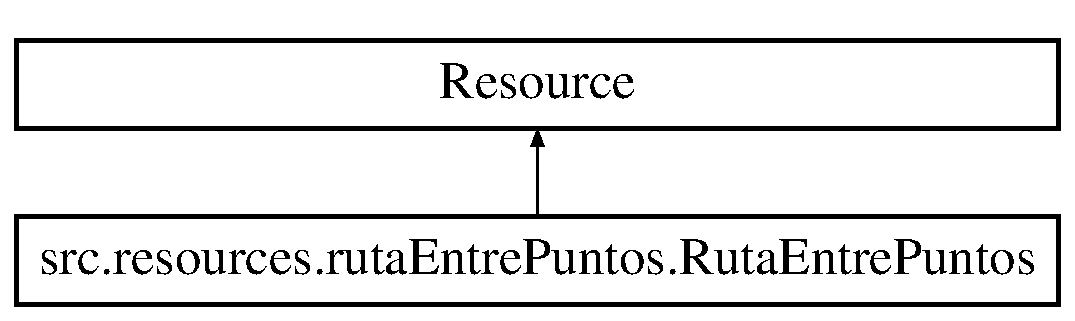
\includegraphics[height=2.000000cm]{classsrc_1_1resources_1_1ruta_entre_puntos_1_1_ruta_entre_puntos}
\end{center}
\end{figure}
\subsection*{Métodos públicos}
\begin{DoxyCompactItemize}
\item 
\hypertarget{classsrc_1_1resources_1_1ruta_entre_puntos_1_1_ruta_entre_puntos_a7fd0962af4dda6c52f4ab1ff6704614f}{def {\bfseries \-\_\-\-\_\-init\-\_\-\-\_\-}}\label{classsrc_1_1resources_1_1ruta_entre_puntos_1_1_ruta_entre_puntos_a7fd0962af4dda6c52f4ab1ff6704614f}

\item 
def \hyperlink{classsrc_1_1resources_1_1ruta_entre_puntos_1_1_ruta_entre_puntos_a14da5f2af9a498be67347a773d11164f}{get}
\begin{DoxyCompactList}\small\item\em Obtiene la ruta entre dos posiciones. \end{DoxyCompactList}\end{DoxyCompactItemize}
\subsection*{Atributos públicos}
\begin{DoxyCompactItemize}
\item 
\hypertarget{classsrc_1_1resources_1_1ruta_entre_puntos_1_1_ruta_entre_puntos_a1df9f4b1f43d71c7d3c08009ec14c328}{{\bfseries autenticador}}\label{classsrc_1_1resources_1_1ruta_entre_puntos_1_1_ruta_entre_puntos_a1df9f4b1f43d71c7d3c08009ec14c328}

\end{DoxyCompactItemize}
\subsection*{Métodos privados}
\begin{DoxyCompactItemize}
\item 
def \hyperlink{classsrc_1_1resources_1_1ruta_entre_puntos_1_1_ruta_entre_puntos_a3390399571b1b0c39b29ef87160a0d12}{\-\_\-get\-\_\-param\-\_\-from\-\_\-request}
\begin{DoxyCompactList}\small\item\em Obtiene el parametro dado de la request. \end{DoxyCompactList}\item 
def \hyperlink{classsrc_1_1resources_1_1ruta_entre_puntos_1_1_ruta_entre_puntos_acccf38dbf6137894b72252c46945de9a}{\-\_\-validate\-\_\-get\-\_\-request}
\begin{DoxyCompactList}\small\item\em Tiene que estar la posicion origen y destino para hacer la busqueda. \end{DoxyCompactList}\item 
def \hyperlink{classsrc_1_1resources_1_1ruta_entre_puntos_1_1_ruta_entre_puntos_a9d20c3e5ef51bbcd883ccff859ecdbaa}{\-\_\-validar\-\_\-token}
\begin{DoxyCompactList}\small\item\em Valida al usuario. \end{DoxyCompactList}\item 
def \hyperlink{classsrc_1_1resources_1_1ruta_entre_puntos_1_1_ruta_entre_puntos_a50b49e766dae726c68021b1e2be2e27a}{\-\_\-acondicionar\-J\-S\-O\-N}
\begin{DoxyCompactList}\small\item\em Acondiciona la salida de Google Directions. \end{DoxyCompactList}\item 
def \hyperlink{classsrc_1_1resources_1_1ruta_entre_puntos_1_1_ruta_entre_puntos_afb5b3a1568a0c6692adf4cbea7f5fcd8}{\-\_\-obtener\-\_\-ruta\-\_\-directions}
\begin{DoxyCompactList}\small\item\em Realiza la peticion a Google Directions. \end{DoxyCompactList}\item 
def \hyperlink{classsrc_1_1resources_1_1ruta_entre_puntos_1_1_ruta_entre_puntos_af12eba89beaa4a98c5c4ab711cf10021}{\-\_\-calcular\-\_\-ruta}
\begin{DoxyCompactList}\small\item\em Pide el servicio a Google Directions. \end{DoxyCompactList}\end{DoxyCompactItemize}


\subsection{Descripción detallada}
Clase para la obtencion entre la ruta entre dos posiciones. 



\subsection{Documentación de las funciones miembro}
\hypertarget{classsrc_1_1resources_1_1ruta_entre_puntos_1_1_ruta_entre_puntos_a50b49e766dae726c68021b1e2be2e27a}{\index{src\-::resources\-::ruta\-Entre\-Puntos\-::\-Ruta\-Entre\-Puntos@{src\-::resources\-::ruta\-Entre\-Puntos\-::\-Ruta\-Entre\-Puntos}!\-\_\-acondicionar\-J\-S\-O\-N@{\-\_\-acondicionar\-J\-S\-O\-N}}
\index{\-\_\-acondicionar\-J\-S\-O\-N@{\-\_\-acondicionar\-J\-S\-O\-N}!src::resources::rutaEntrePuntos::RutaEntrePuntos@{src\-::resources\-::ruta\-Entre\-Puntos\-::\-Ruta\-Entre\-Puntos}}
\subsubsection[{\-\_\-acondicionar\-J\-S\-O\-N}]{\setlength{\rightskip}{0pt plus 5cm}def src.\-resources.\-ruta\-Entre\-Puntos.\-Ruta\-Entre\-Puntos.\-\_\-acondicionar\-J\-S\-O\-N (
\begin{DoxyParamCaption}
\item[{}]{self, }
\item[{}]{datos}
\end{DoxyParamCaption}
)\hspace{0.3cm}{\ttfamily [private]}}}\label{classsrc_1_1resources_1_1ruta_entre_puntos_1_1_ruta_entre_puntos_a50b49e766dae726c68021b1e2be2e27a}


Acondiciona la salida de Google Directions. 


\begin{DoxyParams}{Parámetros}
{\em datos} & Es lo que devuelva Google Directions. \\
\hline
\end{DoxyParams}
\hypertarget{classsrc_1_1resources_1_1ruta_entre_puntos_1_1_ruta_entre_puntos_af12eba89beaa4a98c5c4ab711cf10021}{\index{src\-::resources\-::ruta\-Entre\-Puntos\-::\-Ruta\-Entre\-Puntos@{src\-::resources\-::ruta\-Entre\-Puntos\-::\-Ruta\-Entre\-Puntos}!\-\_\-calcular\-\_\-ruta@{\-\_\-calcular\-\_\-ruta}}
\index{\-\_\-calcular\-\_\-ruta@{\-\_\-calcular\-\_\-ruta}!src::resources::rutaEntrePuntos::RutaEntrePuntos@{src\-::resources\-::ruta\-Entre\-Puntos\-::\-Ruta\-Entre\-Puntos}}
\subsubsection[{\-\_\-calcular\-\_\-ruta}]{\setlength{\rightskip}{0pt plus 5cm}def src.\-resources.\-ruta\-Entre\-Puntos.\-Ruta\-Entre\-Puntos.\-\_\-calcular\-\_\-ruta (
\begin{DoxyParamCaption}
\item[{}]{self, }
\item[{}]{origen, }
\item[{}]{destino}
\end{DoxyParamCaption}
)\hspace{0.3cm}{\ttfamily [private]}}}\label{classsrc_1_1resources_1_1ruta_entre_puntos_1_1_ruta_entre_puntos_af12eba89beaa4a98c5c4ab711cf10021}


Pide el servicio a Google Directions. 

\hypertarget{classsrc_1_1resources_1_1ruta_entre_puntos_1_1_ruta_entre_puntos_a3390399571b1b0c39b29ef87160a0d12}{\index{src\-::resources\-::ruta\-Entre\-Puntos\-::\-Ruta\-Entre\-Puntos@{src\-::resources\-::ruta\-Entre\-Puntos\-::\-Ruta\-Entre\-Puntos}!\-\_\-get\-\_\-param\-\_\-from\-\_\-request@{\-\_\-get\-\_\-param\-\_\-from\-\_\-request}}
\index{\-\_\-get\-\_\-param\-\_\-from\-\_\-request@{\-\_\-get\-\_\-param\-\_\-from\-\_\-request}!src::resources::rutaEntrePuntos::RutaEntrePuntos@{src\-::resources\-::ruta\-Entre\-Puntos\-::\-Ruta\-Entre\-Puntos}}
\subsubsection[{\-\_\-get\-\_\-param\-\_\-from\-\_\-request}]{\setlength{\rightskip}{0pt plus 5cm}def src.\-resources.\-ruta\-Entre\-Puntos.\-Ruta\-Entre\-Puntos.\-\_\-get\-\_\-param\-\_\-from\-\_\-request (
\begin{DoxyParamCaption}
\item[{}]{self, }
\item[{}]{nombre\-Parametro}
\end{DoxyParamCaption}
)\hspace{0.3cm}{\ttfamily [private]}}}\label{classsrc_1_1resources_1_1ruta_entre_puntos_1_1_ruta_entre_puntos_a3390399571b1b0c39b29ef87160a0d12}


Obtiene el parametro dado de la request. 

\hypertarget{classsrc_1_1resources_1_1ruta_entre_puntos_1_1_ruta_entre_puntos_afb5b3a1568a0c6692adf4cbea7f5fcd8}{\index{src\-::resources\-::ruta\-Entre\-Puntos\-::\-Ruta\-Entre\-Puntos@{src\-::resources\-::ruta\-Entre\-Puntos\-::\-Ruta\-Entre\-Puntos}!\-\_\-obtener\-\_\-ruta\-\_\-directions@{\-\_\-obtener\-\_\-ruta\-\_\-directions}}
\index{\-\_\-obtener\-\_\-ruta\-\_\-directions@{\-\_\-obtener\-\_\-ruta\-\_\-directions}!src::resources::rutaEntrePuntos::RutaEntrePuntos@{src\-::resources\-::ruta\-Entre\-Puntos\-::\-Ruta\-Entre\-Puntos}}
\subsubsection[{\-\_\-obtener\-\_\-ruta\-\_\-directions}]{\setlength{\rightskip}{0pt plus 5cm}def src.\-resources.\-ruta\-Entre\-Puntos.\-Ruta\-Entre\-Puntos.\-\_\-obtener\-\_\-ruta\-\_\-directions (
\begin{DoxyParamCaption}
\item[{}]{self, }
\item[{}]{origen, }
\item[{}]{destino}
\end{DoxyParamCaption}
)\hspace{0.3cm}{\ttfamily [private]}}}\label{classsrc_1_1resources_1_1ruta_entre_puntos_1_1_ruta_entre_puntos_afb5b3a1568a0c6692adf4cbea7f5fcd8}


Realiza la peticion a Google Directions. 

\hypertarget{classsrc_1_1resources_1_1ruta_entre_puntos_1_1_ruta_entre_puntos_a9d20c3e5ef51bbcd883ccff859ecdbaa}{\index{src\-::resources\-::ruta\-Entre\-Puntos\-::\-Ruta\-Entre\-Puntos@{src\-::resources\-::ruta\-Entre\-Puntos\-::\-Ruta\-Entre\-Puntos}!\-\_\-validar\-\_\-token@{\-\_\-validar\-\_\-token}}
\index{\-\_\-validar\-\_\-token@{\-\_\-validar\-\_\-token}!src::resources::rutaEntrePuntos::RutaEntrePuntos@{src\-::resources\-::ruta\-Entre\-Puntos\-::\-Ruta\-Entre\-Puntos}}
\subsubsection[{\-\_\-validar\-\_\-token}]{\setlength{\rightskip}{0pt plus 5cm}def src.\-resources.\-ruta\-Entre\-Puntos.\-Ruta\-Entre\-Puntos.\-\_\-validar\-\_\-token (
\begin{DoxyParamCaption}
\item[{}]{self}
\end{DoxyParamCaption}
)\hspace{0.3cm}{\ttfamily [private]}}}\label{classsrc_1_1resources_1_1ruta_entre_puntos_1_1_ruta_entre_puntos_a9d20c3e5ef51bbcd883ccff859ecdbaa}


Valida al usuario. 

\hypertarget{classsrc_1_1resources_1_1ruta_entre_puntos_1_1_ruta_entre_puntos_acccf38dbf6137894b72252c46945de9a}{\index{src\-::resources\-::ruta\-Entre\-Puntos\-::\-Ruta\-Entre\-Puntos@{src\-::resources\-::ruta\-Entre\-Puntos\-::\-Ruta\-Entre\-Puntos}!\-\_\-validate\-\_\-get\-\_\-request@{\-\_\-validate\-\_\-get\-\_\-request}}
\index{\-\_\-validate\-\_\-get\-\_\-request@{\-\_\-validate\-\_\-get\-\_\-request}!src::resources::rutaEntrePuntos::RutaEntrePuntos@{src\-::resources\-::ruta\-Entre\-Puntos\-::\-Ruta\-Entre\-Puntos}}
\subsubsection[{\-\_\-validate\-\_\-get\-\_\-request}]{\setlength{\rightskip}{0pt plus 5cm}def src.\-resources.\-ruta\-Entre\-Puntos.\-Ruta\-Entre\-Puntos.\-\_\-validate\-\_\-get\-\_\-request (
\begin{DoxyParamCaption}
\item[{}]{self}
\end{DoxyParamCaption}
)\hspace{0.3cm}{\ttfamily [private]}}}\label{classsrc_1_1resources_1_1ruta_entre_puntos_1_1_ruta_entre_puntos_acccf38dbf6137894b72252c46945de9a}


Tiene que estar la posicion origen y destino para hacer la busqueda. 

\hypertarget{classsrc_1_1resources_1_1ruta_entre_puntos_1_1_ruta_entre_puntos_a14da5f2af9a498be67347a773d11164f}{\index{src\-::resources\-::ruta\-Entre\-Puntos\-::\-Ruta\-Entre\-Puntos@{src\-::resources\-::ruta\-Entre\-Puntos\-::\-Ruta\-Entre\-Puntos}!get@{get}}
\index{get@{get}!src::resources::rutaEntrePuntos::RutaEntrePuntos@{src\-::resources\-::ruta\-Entre\-Puntos\-::\-Ruta\-Entre\-Puntos}}
\subsubsection[{get}]{\setlength{\rightskip}{0pt plus 5cm}def src.\-resources.\-ruta\-Entre\-Puntos.\-Ruta\-Entre\-Puntos.\-get (
\begin{DoxyParamCaption}
\item[{}]{self}
\end{DoxyParamCaption}
)}}\label{classsrc_1_1resources_1_1ruta_entre_puntos_1_1_ruta_entre_puntos_a14da5f2af9a498be67347a773d11164f}


Obtiene la ruta entre dos posiciones. 



La documentación para esta clase fue generada a partir del siguiente fichero\-:\begin{DoxyCompactItemize}
\item 
src/resources/ruta\-Entre\-Puntos.\-py\end{DoxyCompactItemize}

\hypertarget{classsrc_1_1tests_1_1test__conectividad_1_1_test_conectividad}{\section{Referencia de la Clase src.\-tests.\-test\-\_\-conectividad.\-Test\-Conectividad}
\label{classsrc_1_1tests_1_1test__conectividad_1_1_test_conectividad}\index{src.\-tests.\-test\-\_\-conectividad.\-Test\-Conectividad@{src.\-tests.\-test\-\_\-conectividad.\-Test\-Conectividad}}
}
Diagrama de herencias de src.\-tests.\-test\-\_\-conectividad.\-Test\-Conectividad\begin{figure}[H]
\begin{center}
\leavevmode
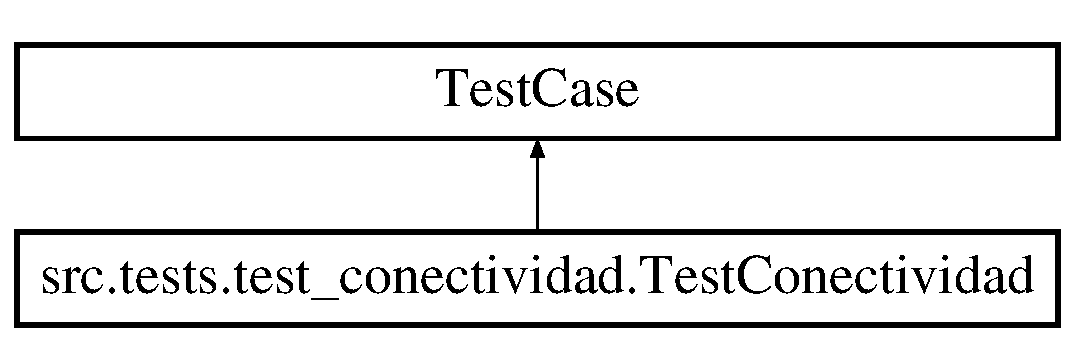
\includegraphics[height=2.000000cm]{classsrc_1_1tests_1_1test__conectividad_1_1_test_conectividad}
\end{center}
\end{figure}
\subsection*{Métodos públicos}
\begin{DoxyCompactItemize}
\item 
\hypertarget{classsrc_1_1tests_1_1test__conectividad_1_1_test_conectividad_ad97b62bf7df1532f58616bf12a2e0b8f}{def {\bfseries test\-\_\-post200\-O\-K}}\label{classsrc_1_1tests_1_1test__conectividad_1_1_test_conectividad_ad97b62bf7df1532f58616bf12a2e0b8f}

\item 
\hypertarget{classsrc_1_1tests_1_1test__conectividad_1_1_test_conectividad_af4869d1e50ef3772d1af78ed658f160a}{def {\bfseries test\-\_\-post\-Mal\-J\-S\-O\-N}}\label{classsrc_1_1tests_1_1test__conectividad_1_1_test_conectividad_af4869d1e50ef3772d1af78ed658f160a}

\item 
\hypertarget{classsrc_1_1tests_1_1test__conectividad_1_1_test_conectividad_a2fcdc3979269ff73e9c438cccba66717}{def {\bfseries test\-\_\-post\-No200}}\label{classsrc_1_1tests_1_1test__conectividad_1_1_test_conectividad_a2fcdc3979269ff73e9c438cccba66717}

\item 
\hypertarget{classsrc_1_1tests_1_1test__conectividad_1_1_test_conectividad_a864cc8f0227de511ba2a77399e6657b5}{def {\bfseries test\-\_\-get200\-O\-K}}\label{classsrc_1_1tests_1_1test__conectividad_1_1_test_conectividad_a864cc8f0227de511ba2a77399e6657b5}

\item 
\hypertarget{classsrc_1_1tests_1_1test__conectividad_1_1_test_conectividad_a0cc4af25c72149bbd92973fb5a3ddf22}{def {\bfseries test\-\_\-get\-Mal\-J\-S\-O\-N}}\label{classsrc_1_1tests_1_1test__conectividad_1_1_test_conectividad_a0cc4af25c72149bbd92973fb5a3ddf22}

\item 
\hypertarget{classsrc_1_1tests_1_1test__conectividad_1_1_test_conectividad_a3efeac84c4b038eae6885cc9c2db23d0}{def {\bfseries test\-\_\-get\-No200}}\label{classsrc_1_1tests_1_1test__conectividad_1_1_test_conectividad_a3efeac84c4b038eae6885cc9c2db23d0}

\item 
\hypertarget{classsrc_1_1tests_1_1test__conectividad_1_1_test_conectividad_aab8bcaa3113924f46cd80c22b03501fe}{def {\bfseries test\-\_\-put200\-O\-K}}\label{classsrc_1_1tests_1_1test__conectividad_1_1_test_conectividad_aab8bcaa3113924f46cd80c22b03501fe}

\item 
\hypertarget{classsrc_1_1tests_1_1test__conectividad_1_1_test_conectividad_a13610804c14418f1678b31d22b534673}{def {\bfseries test\-\_\-put\-Mal\-J\-S\-O\-N}}\label{classsrc_1_1tests_1_1test__conectividad_1_1_test_conectividad_a13610804c14418f1678b31d22b534673}

\item 
\hypertarget{classsrc_1_1tests_1_1test__conectividad_1_1_test_conectividad_a9b93248598f6aa551eb0050563dafb3d}{def {\bfseries test\-\_\-put\-No200}}\label{classsrc_1_1tests_1_1test__conectividad_1_1_test_conectividad_a9b93248598f6aa551eb0050563dafb3d}

\item 
\hypertarget{classsrc_1_1tests_1_1test__conectividad_1_1_test_conectividad_a12a6018f85e7e335a349026020db2051}{def {\bfseries test\-\_\-delete200\-O\-K}}\label{classsrc_1_1tests_1_1test__conectividad_1_1_test_conectividad_a12a6018f85e7e335a349026020db2051}

\item 
\hypertarget{classsrc_1_1tests_1_1test__conectividad_1_1_test_conectividad_a5e7c145fe6d1e8de979634fba5252305}{def {\bfseries test\-\_\-delete\-No200}}\label{classsrc_1_1tests_1_1test__conectividad_1_1_test_conectividad_a5e7c145fe6d1e8de979634fba5252305}

\item 
\hypertarget{classsrc_1_1tests_1_1test__conectividad_1_1_test_conectividad_a9daa32aa5ecb940f33f853b6cb66ecc3}{def {\bfseries test\-\_\-delete200\-Mal\-J\-S\-O\-N}}\label{classsrc_1_1tests_1_1test__conectividad_1_1_test_conectividad_a9daa32aa5ecb940f33f853b6cb66ecc3}

\item 
\hypertarget{classsrc_1_1tests_1_1test__conectividad_1_1_test_conectividad_a7b975f993b7b8a81772f18dd23e5298d}{def {\bfseries test\-\_\-delete\-No200\-Token\-Renovado}}\label{classsrc_1_1tests_1_1test__conectividad_1_1_test_conectividad_a7b975f993b7b8a81772f18dd23e5298d}

\end{DoxyCompactItemize}


La documentación para esta clase fue generada a partir del siguiente fichero\-:\begin{DoxyCompactItemize}
\item 
src/tests/test\-\_\-conectividad.\-py\end{DoxyCompactItemize}

\hypertarget{classsrc_1_1tests_1_1test__endpoint__aceptar_viaje_1_1_test_endpoint_aceptar_viaje}{\section{Referencia de la Clase src.\-tests.\-test\-\_\-endpoint\-\_\-aceptar\-Viaje.\-Test\-Endpoint\-Aceptar\-Viaje}
\label{classsrc_1_1tests_1_1test__endpoint__aceptar_viaje_1_1_test_endpoint_aceptar_viaje}\index{src.\-tests.\-test\-\_\-endpoint\-\_\-aceptar\-Viaje.\-Test\-Endpoint\-Aceptar\-Viaje@{src.\-tests.\-test\-\_\-endpoint\-\_\-aceptar\-Viaje.\-Test\-Endpoint\-Aceptar\-Viaje}}
}
Diagrama de herencias de src.\-tests.\-test\-\_\-endpoint\-\_\-aceptar\-Viaje.\-Test\-Endpoint\-Aceptar\-Viaje\begin{figure}[H]
\begin{center}
\leavevmode
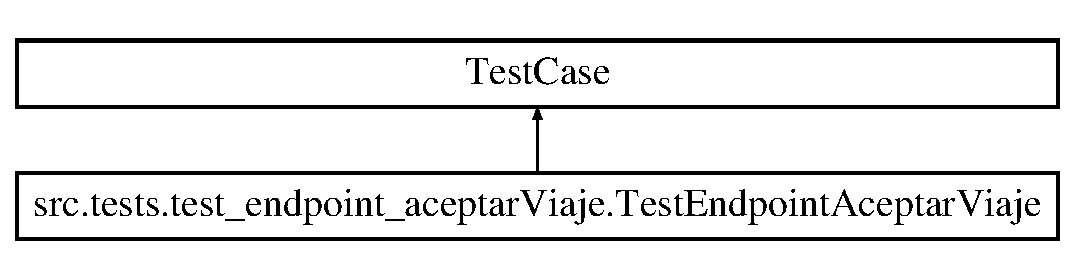
\includegraphics[height=2.000000cm]{classsrc_1_1tests_1_1test__endpoint__aceptar_viaje_1_1_test_endpoint_aceptar_viaje}
\end{center}
\end{figure}
\subsection*{Métodos públicos}
\begin{DoxyCompactItemize}
\item 
\hypertarget{classsrc_1_1tests_1_1test__endpoint__aceptar_viaje_1_1_test_endpoint_aceptar_viaje_a8beab44115fbc8f9e7dd4d327e0897a6}{def {\bfseries set\-Up}}\label{classsrc_1_1tests_1_1test__endpoint__aceptar_viaje_1_1_test_endpoint_aceptar_viaje_a8beab44115fbc8f9e7dd4d327e0897a6}

\item 
\hypertarget{classsrc_1_1tests_1_1test__endpoint__aceptar_viaje_1_1_test_endpoint_aceptar_viaje_a9a025ad053ece7bcd3bc64da725f1879}{def {\bfseries test\-\_\-camino\-\_\-feliz}}\label{classsrc_1_1tests_1_1test__endpoint__aceptar_viaje_1_1_test_endpoint_aceptar_viaje_a9a025ad053ece7bcd3bc64da725f1879}

\item 
\hypertarget{classsrc_1_1tests_1_1test__endpoint__aceptar_viaje_1_1_test_endpoint_aceptar_viaje_a9d570f135421cfaf71a2b84085cfe4d9}{def {\bfseries test\-\_\-token\-\_\-invalido}}\label{classsrc_1_1tests_1_1test__endpoint__aceptar_viaje_1_1_test_endpoint_aceptar_viaje_a9d570f135421cfaf71a2b84085cfe4d9}

\item 
\hypertarget{classsrc_1_1tests_1_1test__endpoint__aceptar_viaje_1_1_test_endpoint_aceptar_viaje_a00a1ce6515d7e5aaef1e2717e757efa3}{def {\bfseries test\-\_\-excepcion\-\_\-viajes\-\_\-find}}\label{classsrc_1_1tests_1_1test__endpoint__aceptar_viaje_1_1_test_endpoint_aceptar_viaje_a00a1ce6515d7e5aaef1e2717e757efa3}

\item 
\hypertarget{classsrc_1_1tests_1_1test__endpoint__aceptar_viaje_1_1_test_endpoint_aceptar_viaje_a0c9e285d3e44b76923a45db49a364636}{def {\bfseries test\-\_\-usuario\-\_\-inexistente}}\label{classsrc_1_1tests_1_1test__endpoint__aceptar_viaje_1_1_test_endpoint_aceptar_viaje_a0c9e285d3e44b76923a45db49a364636}

\item 
\hypertarget{classsrc_1_1tests_1_1test__endpoint__aceptar_viaje_1_1_test_endpoint_aceptar_viaje_a9912eeacb98aa848722af5a6d309ba25}{def {\bfseries test\-\_\-conductor\-\_\-inexistente}}\label{classsrc_1_1tests_1_1test__endpoint__aceptar_viaje_1_1_test_endpoint_aceptar_viaje_a9912eeacb98aa848722af5a6d309ba25}

\item 
\hypertarget{classsrc_1_1tests_1_1test__endpoint__aceptar_viaje_1_1_test_endpoint_aceptar_viaje_a8ba1dbe2d0b62617354eaae022a227e4}{def {\bfseries test\-\_\-update\-\_\-fallido\-\_\-con\-\_\-excepcion}}\label{classsrc_1_1tests_1_1test__endpoint__aceptar_viaje_1_1_test_endpoint_aceptar_viaje_a8ba1dbe2d0b62617354eaae022a227e4}

\end{DoxyCompactItemize}
\subsection*{Atributos públicos}
\begin{DoxyCompactItemize}
\item 
\hypertarget{classsrc_1_1tests_1_1test__endpoint__aceptar_viaje_1_1_test_endpoint_aceptar_viaje_ab1481299733f2664fd6ca8687f924e02}{{\bfseries app}}\label{classsrc_1_1tests_1_1test__endpoint__aceptar_viaje_1_1_test_endpoint_aceptar_viaje_ab1481299733f2664fd6ca8687f924e02}

\item 
\hypertarget{classsrc_1_1tests_1_1test__endpoint__aceptar_viaje_1_1_test_endpoint_aceptar_viaje_ad09d9381f328313f3da897e4c7dafced}{{\bfseries json\-Datos\-Conductor}}\label{classsrc_1_1tests_1_1test__endpoint__aceptar_viaje_1_1_test_endpoint_aceptar_viaje_ad09d9381f328313f3da897e4c7dafced}

\end{DoxyCompactItemize}


La documentación para esta clase fue generada a partir del siguiente fichero\-:\begin{DoxyCompactItemize}
\item 
src/tests/test\-\_\-endpoint\-\_\-aceptar\-Viaje.\-py\end{DoxyCompactItemize}

\hypertarget{classsrc_1_1tests_1_1test__endpoint__agregar_auto_usuario_1_1_test_endpoint_agregar_auto_usuario}{\section{Referencia de la Clase src.\-tests.\-test\-\_\-endpoint\-\_\-agregar\-Auto\-Usuario.\-Test\-Endpoint\-Agregar\-Auto\-Usuario}
\label{classsrc_1_1tests_1_1test__endpoint__agregar_auto_usuario_1_1_test_endpoint_agregar_auto_usuario}\index{src.\-tests.\-test\-\_\-endpoint\-\_\-agregar\-Auto\-Usuario.\-Test\-Endpoint\-Agregar\-Auto\-Usuario@{src.\-tests.\-test\-\_\-endpoint\-\_\-agregar\-Auto\-Usuario.\-Test\-Endpoint\-Agregar\-Auto\-Usuario}}
}
Diagrama de herencias de src.\-tests.\-test\-\_\-endpoint\-\_\-agregar\-Auto\-Usuario.\-Test\-Endpoint\-Agregar\-Auto\-Usuario\begin{figure}[H]
\begin{center}
\leavevmode
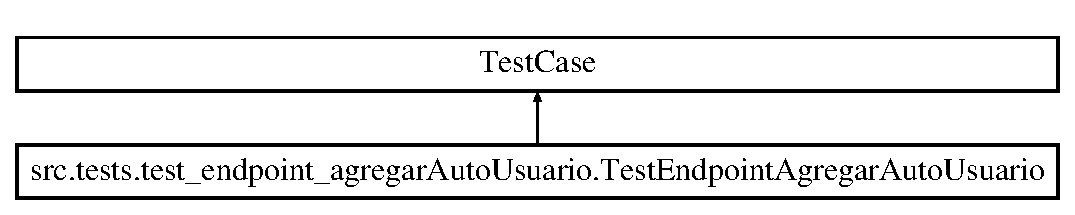
\includegraphics[height=2.000000cm]{classsrc_1_1tests_1_1test__endpoint__agregar_auto_usuario_1_1_test_endpoint_agregar_auto_usuario}
\end{center}
\end{figure}
\subsection*{Métodos públicos}
\begin{DoxyCompactItemize}
\item 
\hypertarget{classsrc_1_1tests_1_1test__endpoint__agregar_auto_usuario_1_1_test_endpoint_agregar_auto_usuario_aacb6afd67143d3c3705364c87c0e5849}{def {\bfseries set\-Up}}\label{classsrc_1_1tests_1_1test__endpoint__agregar_auto_usuario_1_1_test_endpoint_agregar_auto_usuario_aacb6afd67143d3c3705364c87c0e5849}

\item 
\hypertarget{classsrc_1_1tests_1_1test__endpoint__agregar_auto_usuario_1_1_test_endpoint_agregar_auto_usuario_a8253a72937ffba040c1f1db102dac362}{def {\bfseries test\-\_\-camino\-\_\-feliz}}\label{classsrc_1_1tests_1_1test__endpoint__agregar_auto_usuario_1_1_test_endpoint_agregar_auto_usuario_a8253a72937ffba040c1f1db102dac362}

\item 
\hypertarget{classsrc_1_1tests_1_1test__endpoint__agregar_auto_usuario_1_1_test_endpoint_agregar_auto_usuario_aced52b20e0bac60768d3e47d0c72b932}{def {\bfseries test\-\_\-sin\-\_\-token}}\label{classsrc_1_1tests_1_1test__endpoint__agregar_auto_usuario_1_1_test_endpoint_agregar_auto_usuario_aced52b20e0bac60768d3e47d0c72b932}

\item 
\hypertarget{classsrc_1_1tests_1_1test__endpoint__agregar_auto_usuario_1_1_test_endpoint_agregar_auto_usuario_aca3908b8a9de80c36eeb0e822256e182}{def {\bfseries test\-\_\-sin\-\_\-json}}\label{classsrc_1_1tests_1_1test__endpoint__agregar_auto_usuario_1_1_test_endpoint_agregar_auto_usuario_aca3908b8a9de80c36eeb0e822256e182}

\item 
\hypertarget{classsrc_1_1tests_1_1test__endpoint__agregar_auto_usuario_1_1_test_endpoint_agregar_auto_usuario_a47544aa1cc585bc45e3ec6e1ab805976}{def {\bfseries test\-\_\-token\-\_\-invalido}}\label{classsrc_1_1tests_1_1test__endpoint__agregar_auto_usuario_1_1_test_endpoint_agregar_auto_usuario_a47544aa1cc585bc45e3ec6e1ab805976}

\item 
\hypertarget{classsrc_1_1tests_1_1test__endpoint__agregar_auto_usuario_1_1_test_endpoint_agregar_auto_usuario_aa36d560f4902380e48d4d49c6e689ee7}{def {\bfseries test\-\_\-conexion\-\_\-fallida}}\label{classsrc_1_1tests_1_1test__endpoint__agregar_auto_usuario_1_1_test_endpoint_agregar_auto_usuario_aa36d560f4902380e48d4d49c6e689ee7}

\end{DoxyCompactItemize}
\subsection*{Atributos públicos}
\begin{DoxyCompactItemize}
\item 
\hypertarget{classsrc_1_1tests_1_1test__endpoint__agregar_auto_usuario_1_1_test_endpoint_agregar_auto_usuario_ae6c82cc1c1576393ebf5710ac53bd680}{{\bfseries app}}\label{classsrc_1_1tests_1_1test__endpoint__agregar_auto_usuario_1_1_test_endpoint_agregar_auto_usuario_ae6c82cc1c1576393ebf5710ac53bd680}

\end{DoxyCompactItemize}


La documentación para esta clase fue generada a partir del siguiente fichero\-:\begin{DoxyCompactItemize}
\item 
src/tests/test\-\_\-endpoint\-\_\-agregar\-Auto\-Usuario.\-py\end{DoxyCompactItemize}

\hypertarget{classsrc_1_1tests_1_1test__endpoint__agregar_posible_viaje_1_1_test_endpoint_agregar_posible_viaje}{\section{Referencia de la Clase src.\-tests.\-test\-\_\-endpoint\-\_\-agregar\-Posible\-Viaje.\-Test\-Endpoint\-Agregar\-Posible\-Viaje}
\label{classsrc_1_1tests_1_1test__endpoint__agregar_posible_viaje_1_1_test_endpoint_agregar_posible_viaje}\index{src.\-tests.\-test\-\_\-endpoint\-\_\-agregar\-Posible\-Viaje.\-Test\-Endpoint\-Agregar\-Posible\-Viaje@{src.\-tests.\-test\-\_\-endpoint\-\_\-agregar\-Posible\-Viaje.\-Test\-Endpoint\-Agregar\-Posible\-Viaje}}
}
Diagrama de herencias de src.\-tests.\-test\-\_\-endpoint\-\_\-agregar\-Posible\-Viaje.\-Test\-Endpoint\-Agregar\-Posible\-Viaje\begin{figure}[H]
\begin{center}
\leavevmode
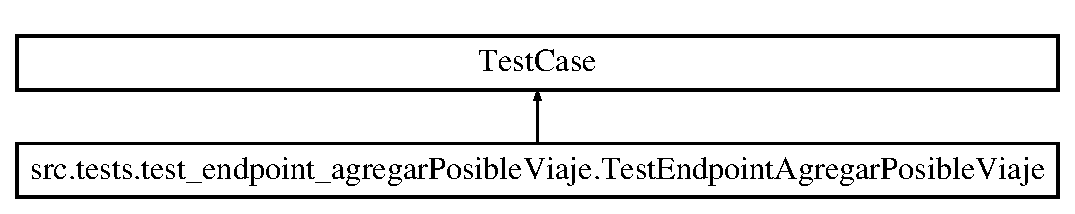
\includegraphics[height=2.000000cm]{classsrc_1_1tests_1_1test__endpoint__agregar_posible_viaje_1_1_test_endpoint_agregar_posible_viaje}
\end{center}
\end{figure}
\subsection*{Métodos públicos}
\begin{DoxyCompactItemize}
\item 
\hypertarget{classsrc_1_1tests_1_1test__endpoint__agregar_posible_viaje_1_1_test_endpoint_agregar_posible_viaje_ae37d0e9f1d9affa8dc009e3b12eca454}{def {\bfseries set\-Up}}\label{classsrc_1_1tests_1_1test__endpoint__agregar_posible_viaje_1_1_test_endpoint_agregar_posible_viaje_ae37d0e9f1d9affa8dc009e3b12eca454}

\item 
\hypertarget{classsrc_1_1tests_1_1test__endpoint__agregar_posible_viaje_1_1_test_endpoint_agregar_posible_viaje_a94024bac1a5d33140db0811f2a08e262}{def {\bfseries get\-Normal}}\label{classsrc_1_1tests_1_1test__endpoint__agregar_posible_viaje_1_1_test_endpoint_agregar_posible_viaje_a94024bac1a5d33140db0811f2a08e262}

\item 
\hypertarget{classsrc_1_1tests_1_1test__endpoint__agregar_posible_viaje_1_1_test_endpoint_agregar_posible_viaje_a3704f3eb0dc802f9e3b9055db4ceb7b3}{def {\bfseries get\-Fallido\-Segunda\-Excepcion}}\label{classsrc_1_1tests_1_1test__endpoint__agregar_posible_viaje_1_1_test_endpoint_agregar_posible_viaje_a3704f3eb0dc802f9e3b9055db4ceb7b3}

\item 
\hypertarget{classsrc_1_1tests_1_1test__endpoint__agregar_posible_viaje_1_1_test_endpoint_agregar_posible_viaje_ac315599fdf63dac17d8b51813dd00568}{def {\bfseries get\-Fallido\-Segunda\-False}}\label{classsrc_1_1tests_1_1test__endpoint__agregar_posible_viaje_1_1_test_endpoint_agregar_posible_viaje_ac315599fdf63dac17d8b51813dd00568}

\item 
\hypertarget{classsrc_1_1tests_1_1test__endpoint__agregar_posible_viaje_1_1_test_endpoint_agregar_posible_viaje_a2eca9e0c799f3fff28c7a3fbb1c6f89c}{def {\bfseries test\-\_\-camino\-\_\-feliz}}\label{classsrc_1_1tests_1_1test__endpoint__agregar_posible_viaje_1_1_test_endpoint_agregar_posible_viaje_a2eca9e0c799f3fff28c7a3fbb1c6f89c}

\item 
\hypertarget{classsrc_1_1tests_1_1test__endpoint__agregar_posible_viaje_1_1_test_endpoint_agregar_posible_viaje_a7f45b399539ada9075cdd666aecfab11}{def {\bfseries test\-\_\-sin\-\_\-json}}\label{classsrc_1_1tests_1_1test__endpoint__agregar_posible_viaje_1_1_test_endpoint_agregar_posible_viaje_a7f45b399539ada9075cdd666aecfab11}

\item 
\hypertarget{classsrc_1_1tests_1_1test__endpoint__agregar_posible_viaje_1_1_test_endpoint_agregar_posible_viaje_aa1dafb37a0abb43a940bbe4e909f3754}{def {\bfseries test\-\_\-token\-\_\-invalido}}\label{classsrc_1_1tests_1_1test__endpoint__agregar_posible_viaje_1_1_test_endpoint_agregar_posible_viaje_aa1dafb37a0abb43a940bbe4e909f3754}

\item 
\hypertarget{classsrc_1_1tests_1_1test__endpoint__agregar_posible_viaje_1_1_test_endpoint_agregar_posible_viaje_a52ccc58f12c3d7a8402a5229dd02c534}{def {\bfseries test\-\_\-estimacion\-\_\-fallida}}\label{classsrc_1_1tests_1_1test__endpoint__agregar_posible_viaje_1_1_test_endpoint_agregar_posible_viaje_a52ccc58f12c3d7a8402a5229dd02c534}

\item 
\hypertarget{classsrc_1_1tests_1_1test__endpoint__agregar_posible_viaje_1_1_test_endpoint_agregar_posible_viaje_a039cd628781df40aa2def5f6df3844c7}{def {\bfseries test\-\_\-pasajero\-\_\-inexistente}}\label{classsrc_1_1tests_1_1test__endpoint__agregar_posible_viaje_1_1_test_endpoint_agregar_posible_viaje_a039cd628781df40aa2def5f6df3844c7}

\item 
\hypertarget{classsrc_1_1tests_1_1test__endpoint__agregar_posible_viaje_1_1_test_endpoint_agregar_posible_viaje_a3533bfab165d9d9b8b287eb4d1a65bb5}{def {\bfseries test\-\_\-fallo\-\_\-al\-\_\-guardar\-\_\-mongodb}}\label{classsrc_1_1tests_1_1test__endpoint__agregar_posible_viaje_1_1_test_endpoint_agregar_posible_viaje_a3533bfab165d9d9b8b287eb4d1a65bb5}

\item 
\hypertarget{classsrc_1_1tests_1_1test__endpoint__agregar_posible_viaje_1_1_test_endpoint_agregar_posible_viaje_a325fa357d0aa1cfdb0410a21ae8ea152}{def {\bfseries test\-\_\-fallo\-\_\-al\-\_\-guardar\-\_\-mongodb\-\_\-excepcion}}\label{classsrc_1_1tests_1_1test__endpoint__agregar_posible_viaje_1_1_test_endpoint_agregar_posible_viaje_a325fa357d0aa1cfdb0410a21ae8ea152}

\item 
\hypertarget{classsrc_1_1tests_1_1test__endpoint__agregar_posible_viaje_1_1_test_endpoint_agregar_posible_viaje_afd377d975b510a457ee0cfc7ea50d439}{def {\bfseries test\-\_\-fallo\-\_\-al\-\_\-obtener\-\_\-ruta\-\_\-excepcion}}\label{classsrc_1_1tests_1_1test__endpoint__agregar_posible_viaje_1_1_test_endpoint_agregar_posible_viaje_afd377d975b510a457ee0cfc7ea50d439}

\item 
\hypertarget{classsrc_1_1tests_1_1test__endpoint__agregar_posible_viaje_1_1_test_endpoint_agregar_posible_viaje_a56aef0ca70267663077608633c204ef4}{def {\bfseries test\-\_\-fallo\-\_\-al\-\_\-obtener\-\_\-ruta\-\_\-false}}\label{classsrc_1_1tests_1_1test__endpoint__agregar_posible_viaje_1_1_test_endpoint_agregar_posible_viaje_a56aef0ca70267663077608633c204ef4}

\end{DoxyCompactItemize}
\subsection*{Atributos públicos}
\begin{DoxyCompactItemize}
\item 
\hypertarget{classsrc_1_1tests_1_1test__endpoint__agregar_posible_viaje_1_1_test_endpoint_agregar_posible_viaje_ab48398059e7f2ce4eb9e299605865fb0}{{\bfseries app}}\label{classsrc_1_1tests_1_1test__endpoint__agregar_posible_viaje_1_1_test_endpoint_agregar_posible_viaje_ab48398059e7f2ce4eb9e299605865fb0}

\item 
\hypertarget{classsrc_1_1tests_1_1test__endpoint__agregar_posible_viaje_1_1_test_endpoint_agregar_posible_viaje_a7054b644acc7c503a9ad06325b884f19}{{\bfseries estimacion}}\label{classsrc_1_1tests_1_1test__endpoint__agregar_posible_viaje_1_1_test_endpoint_agregar_posible_viaje_a7054b644acc7c503a9ad06325b884f19}

\item 
\hypertarget{classsrc_1_1tests_1_1test__endpoint__agregar_posible_viaje_1_1_test_endpoint_agregar_posible_viaje_a3ea88183ffef7e86b255a90b7e326473}{{\bfseries datos\-Pasajero}}\label{classsrc_1_1tests_1_1test__endpoint__agregar_posible_viaje_1_1_test_endpoint_agregar_posible_viaje_a3ea88183ffef7e86b255a90b7e326473}

\item 
\hypertarget{classsrc_1_1tests_1_1test__endpoint__agregar_posible_viaje_1_1_test_endpoint_agregar_posible_viaje_aae380d4b211a2200b599fcbb66e1904a}{{\bfseries datos\-Directions}}\label{classsrc_1_1tests_1_1test__endpoint__agregar_posible_viaje_1_1_test_endpoint_agregar_posible_viaje_aae380d4b211a2200b599fcbb66e1904a}

\end{DoxyCompactItemize}


La documentación para esta clase fue generada a partir del siguiente fichero\-:\begin{DoxyCompactItemize}
\item 
src/tests/test\-\_\-endpoint\-\_\-agregar\-Posible\-Viaje.\-py\end{DoxyCompactItemize}

\hypertarget{classsrc_1_1tests_1_1test__endpoint__auto_por_i_d_1_1_test_endpoint_auto_por_i_d}{\section{Referencia de la Clase src.\-tests.\-test\-\_\-endpoint\-\_\-auto\-Por\-I\-D.\-Test\-Endpoint\-Auto\-Por\-I\-D}
\label{classsrc_1_1tests_1_1test__endpoint__auto_por_i_d_1_1_test_endpoint_auto_por_i_d}\index{src.\-tests.\-test\-\_\-endpoint\-\_\-auto\-Por\-I\-D.\-Test\-Endpoint\-Auto\-Por\-I\-D@{src.\-tests.\-test\-\_\-endpoint\-\_\-auto\-Por\-I\-D.\-Test\-Endpoint\-Auto\-Por\-I\-D}}
}
Diagrama de herencias de src.\-tests.\-test\-\_\-endpoint\-\_\-auto\-Por\-I\-D.\-Test\-Endpoint\-Auto\-Por\-I\-D\begin{figure}[H]
\begin{center}
\leavevmode
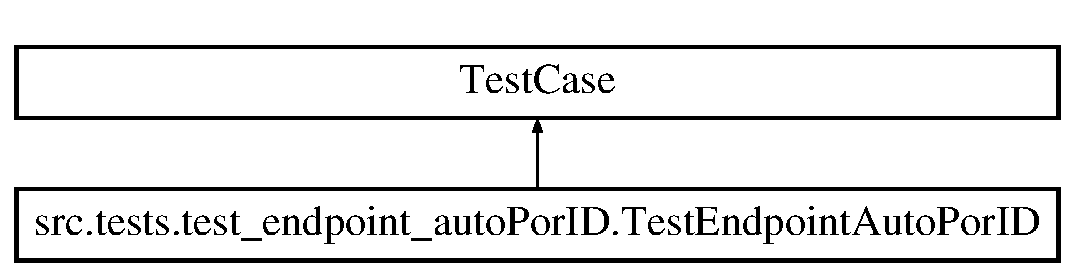
\includegraphics[height=2.000000cm]{classsrc_1_1tests_1_1test__endpoint__auto_por_i_d_1_1_test_endpoint_auto_por_i_d}
\end{center}
\end{figure}
\subsection*{Métodos públicos}
\begin{DoxyCompactItemize}
\item 
\hypertarget{classsrc_1_1tests_1_1test__endpoint__auto_por_i_d_1_1_test_endpoint_auto_por_i_d_a285971f8807370c1fa4bd6c7effcd6f1}{def {\bfseries set\-Up}}\label{classsrc_1_1tests_1_1test__endpoint__auto_por_i_d_1_1_test_endpoint_auto_por_i_d_a285971f8807370c1fa4bd6c7effcd6f1}

\item 
\hypertarget{classsrc_1_1tests_1_1test__endpoint__auto_por_i_d_1_1_test_endpoint_auto_por_i_d_af78c8558cf88684384ed6a5996d657fb}{def {\bfseries test\-\_\-camino\-\_\-feliz}}\label{classsrc_1_1tests_1_1test__endpoint__auto_por_i_d_1_1_test_endpoint_auto_por_i_d_af78c8558cf88684384ed6a5996d657fb}

\item 
\hypertarget{classsrc_1_1tests_1_1test__endpoint__auto_por_i_d_1_1_test_endpoint_auto_por_i_d_a5b3b8fc1a23fe86dc17b77dd24ac540c}{def {\bfseries test\-\_\-sin\-\_\-token}}\label{classsrc_1_1tests_1_1test__endpoint__auto_por_i_d_1_1_test_endpoint_auto_por_i_d_a5b3b8fc1a23fe86dc17b77dd24ac540c}

\item 
\hypertarget{classsrc_1_1tests_1_1test__endpoint__auto_por_i_d_1_1_test_endpoint_auto_por_i_d_a96dd6e9682e4c6de674abc61fa582fbd}{def {\bfseries test\-\_\-token\-\_\-invalido}}\label{classsrc_1_1tests_1_1test__endpoint__auto_por_i_d_1_1_test_endpoint_auto_por_i_d_a96dd6e9682e4c6de674abc61fa582fbd}

\item 
\hypertarget{classsrc_1_1tests_1_1test__endpoint__auto_por_i_d_1_1_test_endpoint_auto_por_i_d_a5d55a58bb4b9191aa97d47e16b708b37}{def {\bfseries test\-\_\-conexion\-\_\-fallida}}\label{classsrc_1_1tests_1_1test__endpoint__auto_por_i_d_1_1_test_endpoint_auto_por_i_d_a5d55a58bb4b9191aa97d47e16b708b37}

\end{DoxyCompactItemize}
\subsection*{Atributos públicos}
\begin{DoxyCompactItemize}
\item 
\hypertarget{classsrc_1_1tests_1_1test__endpoint__auto_por_i_d_1_1_test_endpoint_auto_por_i_d_a0ca8239725f94499916f1b151ae7f560}{{\bfseries app}}\label{classsrc_1_1tests_1_1test__endpoint__auto_por_i_d_1_1_test_endpoint_auto_por_i_d_a0ca8239725f94499916f1b151ae7f560}

\end{DoxyCompactItemize}


La documentación para esta clase fue generada a partir del siguiente fichero\-:\begin{DoxyCompactItemize}
\item 
src/tests/test\-\_\-endpoint\-\_\-auto\-Por\-I\-D.\-py\end{DoxyCompactItemize}

\hypertarget{classsrc_1_1tests_1_1test__endpoint__autos_por_posicion_cercana_1_1_test_endpoint_autos_por_posicion_cercana}{\section{Referencia de la Clase src.\-tests.\-test\-\_\-endpoint\-\_\-autos\-Por\-Posicion\-Cercana.\-Test\-Endpoint\-Autos\-Por\-Posicion\-Cercana}
\label{classsrc_1_1tests_1_1test__endpoint__autos_por_posicion_cercana_1_1_test_endpoint_autos_por_posicion_cercana}\index{src.\-tests.\-test\-\_\-endpoint\-\_\-autos\-Por\-Posicion\-Cercana.\-Test\-Endpoint\-Autos\-Por\-Posicion\-Cercana@{src.\-tests.\-test\-\_\-endpoint\-\_\-autos\-Por\-Posicion\-Cercana.\-Test\-Endpoint\-Autos\-Por\-Posicion\-Cercana}}
}
Diagrama de herencias de src.\-tests.\-test\-\_\-endpoint\-\_\-autos\-Por\-Posicion\-Cercana.\-Test\-Endpoint\-Autos\-Por\-Posicion\-Cercana\begin{figure}[H]
\begin{center}
\leavevmode
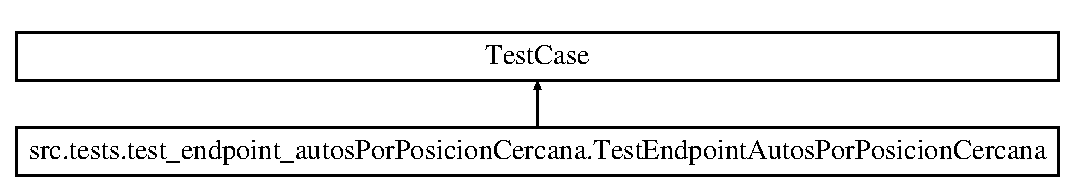
\includegraphics[height=2.000000cm]{classsrc_1_1tests_1_1test__endpoint__autos_por_posicion_cercana_1_1_test_endpoint_autos_por_posicion_cercana}
\end{center}
\end{figure}
\subsection*{Métodos públicos}
\begin{DoxyCompactItemize}
\item 
\hypertarget{classsrc_1_1tests_1_1test__endpoint__autos_por_posicion_cercana_1_1_test_endpoint_autos_por_posicion_cercana_a9af3d0a1d78753c9d057a71d550b3f70}{def {\bfseries set\-Up}}\label{classsrc_1_1tests_1_1test__endpoint__autos_por_posicion_cercana_1_1_test_endpoint_autos_por_posicion_cercana_a9af3d0a1d78753c9d057a71d550b3f70}

\item 
\hypertarget{classsrc_1_1tests_1_1test__endpoint__autos_por_posicion_cercana_1_1_test_endpoint_autos_por_posicion_cercana_a1bfe6984fa124d5a3d7ec10635fbc794}{def {\bfseries test\-\_\-camino\-\_\-feliz}}\label{classsrc_1_1tests_1_1test__endpoint__autos_por_posicion_cercana_1_1_test_endpoint_autos_por_posicion_cercana_a1bfe6984fa124d5a3d7ec10635fbc794}

\item 
\hypertarget{classsrc_1_1tests_1_1test__endpoint__autos_por_posicion_cercana_1_1_test_endpoint_autos_por_posicion_cercana_a82da05aa23f4ebcca0b8c8acab6390fb}{def {\bfseries test\-\_\-sin\-\_\-lat\-\_\-y\-\_\-lng}}\label{classsrc_1_1tests_1_1test__endpoint__autos_por_posicion_cercana_1_1_test_endpoint_autos_por_posicion_cercana_a82da05aa23f4ebcca0b8c8acab6390fb}

\item 
\hypertarget{classsrc_1_1tests_1_1test__endpoint__autos_por_posicion_cercana_1_1_test_endpoint_autos_por_posicion_cercana_a7e7adf43593a098f8c28a6bcb81fc7cc}{def {\bfseries test\-\_\-sin\-\_\-token}}\label{classsrc_1_1tests_1_1test__endpoint__autos_por_posicion_cercana_1_1_test_endpoint_autos_por_posicion_cercana_a7e7adf43593a098f8c28a6bcb81fc7cc}

\item 
\hypertarget{classsrc_1_1tests_1_1test__endpoint__autos_por_posicion_cercana_1_1_test_endpoint_autos_por_posicion_cercana_a1244c763ddfdfe28a75c7939a3701c7b}{def {\bfseries test\-\_\-token\-\_\-invalido}}\label{classsrc_1_1tests_1_1test__endpoint__autos_por_posicion_cercana_1_1_test_endpoint_autos_por_posicion_cercana_a1244c763ddfdfe28a75c7939a3701c7b}

\item 
\hypertarget{classsrc_1_1tests_1_1test__endpoint__autos_por_posicion_cercana_1_1_test_endpoint_autos_por_posicion_cercana_a822e97263311da7f64911b738b333ef2}{def {\bfseries test\-\_\-conexion\-\_\-fallida}}\label{classsrc_1_1tests_1_1test__endpoint__autos_por_posicion_cercana_1_1_test_endpoint_autos_por_posicion_cercana_a822e97263311da7f64911b738b333ef2}

\end{DoxyCompactItemize}
\subsection*{Atributos públicos}
\begin{DoxyCompactItemize}
\item 
\hypertarget{classsrc_1_1tests_1_1test__endpoint__autos_por_posicion_cercana_1_1_test_endpoint_autos_por_posicion_cercana_aeb3b20e83a148ecec20d537719adea86}{{\bfseries app}}\label{classsrc_1_1tests_1_1test__endpoint__autos_por_posicion_cercana_1_1_test_endpoint_autos_por_posicion_cercana_aeb3b20e83a148ecec20d537719adea86}

\end{DoxyCompactItemize}


La documentación para esta clase fue generada a partir del siguiente fichero\-:\begin{DoxyCompactItemize}
\item 
src/tests/test\-\_\-endpoint\-\_\-autos\-Por\-Posicion\-Cercana.\-py\end{DoxyCompactItemize}

\hypertarget{classsrc_1_1tests_1_1test__endpoint__autos_por_usuario_1_1_test_endpoint_autos_por_usuario}{\section{Referencia de la Clase src.\-tests.\-test\-\_\-endpoint\-\_\-autos\-Por\-Usuario.\-Test\-Endpoint\-Autos\-Por\-Usuario}
\label{classsrc_1_1tests_1_1test__endpoint__autos_por_usuario_1_1_test_endpoint_autos_por_usuario}\index{src.\-tests.\-test\-\_\-endpoint\-\_\-autos\-Por\-Usuario.\-Test\-Endpoint\-Autos\-Por\-Usuario@{src.\-tests.\-test\-\_\-endpoint\-\_\-autos\-Por\-Usuario.\-Test\-Endpoint\-Autos\-Por\-Usuario}}
}
Diagrama de herencias de src.\-tests.\-test\-\_\-endpoint\-\_\-autos\-Por\-Usuario.\-Test\-Endpoint\-Autos\-Por\-Usuario\begin{figure}[H]
\begin{center}
\leavevmode
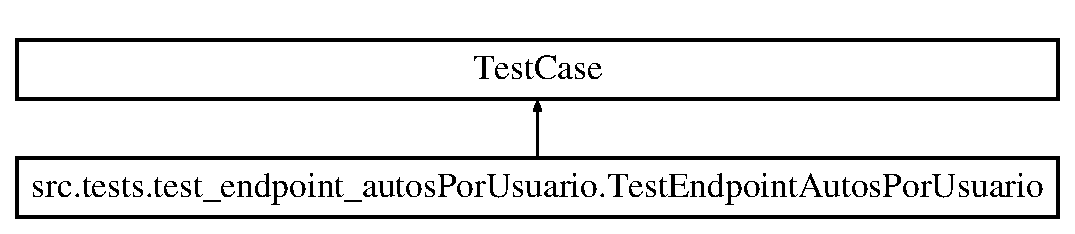
\includegraphics[height=2.000000cm]{classsrc_1_1tests_1_1test__endpoint__autos_por_usuario_1_1_test_endpoint_autos_por_usuario}
\end{center}
\end{figure}
\subsection*{Métodos públicos}
\begin{DoxyCompactItemize}
\item 
\hypertarget{classsrc_1_1tests_1_1test__endpoint__autos_por_usuario_1_1_test_endpoint_autos_por_usuario_a3a4a1f4eaf7c91de538f0da6fb3a1982}{def {\bfseries set\-Up}}\label{classsrc_1_1tests_1_1test__endpoint__autos_por_usuario_1_1_test_endpoint_autos_por_usuario_a3a4a1f4eaf7c91de538f0da6fb3a1982}

\item 
\hypertarget{classsrc_1_1tests_1_1test__endpoint__autos_por_usuario_1_1_test_endpoint_autos_por_usuario_a81f833a96aa23aa8e2c96ef89afdaf64}{def {\bfseries test\-\_\-camino\-\_\-feliz}}\label{classsrc_1_1tests_1_1test__endpoint__autos_por_usuario_1_1_test_endpoint_autos_por_usuario_a81f833a96aa23aa8e2c96ef89afdaf64}

\item 
\hypertarget{classsrc_1_1tests_1_1test__endpoint__autos_por_usuario_1_1_test_endpoint_autos_por_usuario_a370a382ec1951a14be8cae43e0193ad6}{def {\bfseries test\-\_\-sin\-\_\-token}}\label{classsrc_1_1tests_1_1test__endpoint__autos_por_usuario_1_1_test_endpoint_autos_por_usuario_a370a382ec1951a14be8cae43e0193ad6}

\item 
\hypertarget{classsrc_1_1tests_1_1test__endpoint__autos_por_usuario_1_1_test_endpoint_autos_por_usuario_acfc970c6e00e009bd9082756be6dc9fd}{def {\bfseries test\-\_\-token\-\_\-invalido}}\label{classsrc_1_1tests_1_1test__endpoint__autos_por_usuario_1_1_test_endpoint_autos_por_usuario_acfc970c6e00e009bd9082756be6dc9fd}

\item 
\hypertarget{classsrc_1_1tests_1_1test__endpoint__autos_por_usuario_1_1_test_endpoint_autos_por_usuario_ace2136745a04641ef19b0385e66d40f9}{def {\bfseries test\-\_\-conexion\-\_\-fallida}}\label{classsrc_1_1tests_1_1test__endpoint__autos_por_usuario_1_1_test_endpoint_autos_por_usuario_ace2136745a04641ef19b0385e66d40f9}

\end{DoxyCompactItemize}
\subsection*{Atributos públicos}
\begin{DoxyCompactItemize}
\item 
\hypertarget{classsrc_1_1tests_1_1test__endpoint__autos_por_usuario_1_1_test_endpoint_autos_por_usuario_af2da830c2fb295032fc7d5bd93cc86a8}{{\bfseries app}}\label{classsrc_1_1tests_1_1test__endpoint__autos_por_usuario_1_1_test_endpoint_autos_por_usuario_af2da830c2fb295032fc7d5bd93cc86a8}

\end{DoxyCompactItemize}


La documentación para esta clase fue generada a partir del siguiente fichero\-:\begin{DoxyCompactItemize}
\item 
src/tests/test\-\_\-endpoint\-\_\-autos\-Por\-Usuario.\-py\end{DoxyCompactItemize}

\hypertarget{classsrc_1_1tests_1_1test__endpoint__eliminar_auto_usuario_1_1_test_endpoint_eliminar_auto_usuario}{\section{Referencia de la Clase src.\-tests.\-test\-\_\-endpoint\-\_\-eliminar\-Auto\-Usuario.\-Test\-Endpoint\-Eliminar\-Auto\-Usuario}
\label{classsrc_1_1tests_1_1test__endpoint__eliminar_auto_usuario_1_1_test_endpoint_eliminar_auto_usuario}\index{src.\-tests.\-test\-\_\-endpoint\-\_\-eliminar\-Auto\-Usuario.\-Test\-Endpoint\-Eliminar\-Auto\-Usuario@{src.\-tests.\-test\-\_\-endpoint\-\_\-eliminar\-Auto\-Usuario.\-Test\-Endpoint\-Eliminar\-Auto\-Usuario}}
}
Diagrama de herencias de src.\-tests.\-test\-\_\-endpoint\-\_\-eliminar\-Auto\-Usuario.\-Test\-Endpoint\-Eliminar\-Auto\-Usuario\begin{figure}[H]
\begin{center}
\leavevmode
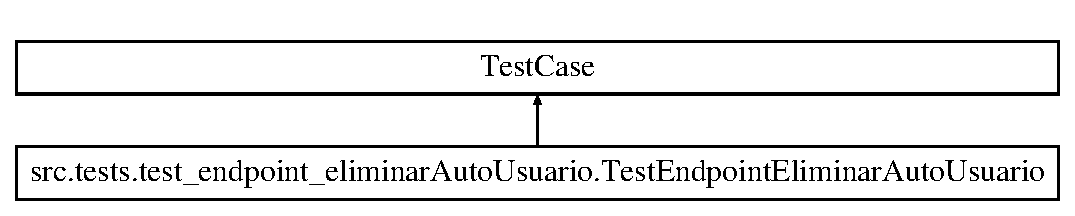
\includegraphics[height=2.000000cm]{classsrc_1_1tests_1_1test__endpoint__eliminar_auto_usuario_1_1_test_endpoint_eliminar_auto_usuario}
\end{center}
\end{figure}
\subsection*{Métodos públicos}
\begin{DoxyCompactItemize}
\item 
\hypertarget{classsrc_1_1tests_1_1test__endpoint__eliminar_auto_usuario_1_1_test_endpoint_eliminar_auto_usuario_af1c8d2726251de97f8b6a48b7de99863}{def {\bfseries set\-Up}}\label{classsrc_1_1tests_1_1test__endpoint__eliminar_auto_usuario_1_1_test_endpoint_eliminar_auto_usuario_af1c8d2726251de97f8b6a48b7de99863}

\item 
\hypertarget{classsrc_1_1tests_1_1test__endpoint__eliminar_auto_usuario_1_1_test_endpoint_eliminar_auto_usuario_acfa8784062cf572dfd1e7f7f536757f3}{def {\bfseries test\-\_\-camino\-\_\-feliz}}\label{classsrc_1_1tests_1_1test__endpoint__eliminar_auto_usuario_1_1_test_endpoint_eliminar_auto_usuario_acfa8784062cf572dfd1e7f7f536757f3}

\item 
\hypertarget{classsrc_1_1tests_1_1test__endpoint__eliminar_auto_usuario_1_1_test_endpoint_eliminar_auto_usuario_a76bbb67fdc9ead13f92e767bbbb31061}{def {\bfseries test\-\_\-camino\-\_\-feliz\-\_\-sin\-\_\-autos\-\_\-al\-\_\-final}}\label{classsrc_1_1tests_1_1test__endpoint__eliminar_auto_usuario_1_1_test_endpoint_eliminar_auto_usuario_a76bbb67fdc9ead13f92e767bbbb31061}

\item 
\hypertarget{classsrc_1_1tests_1_1test__endpoint__eliminar_auto_usuario_1_1_test_endpoint_eliminar_auto_usuario_a2132886ba256f862f41a2ced95135264}{def {\bfseries test\-\_\-sin\-\_\-token}}\label{classsrc_1_1tests_1_1test__endpoint__eliminar_auto_usuario_1_1_test_endpoint_eliminar_auto_usuario_a2132886ba256f862f41a2ced95135264}

\item 
\hypertarget{classsrc_1_1tests_1_1test__endpoint__eliminar_auto_usuario_1_1_test_endpoint_eliminar_auto_usuario_af83c93ae26a82afad736a86420281629}{def {\bfseries test\-\_\-token\-\_\-invalido}}\label{classsrc_1_1tests_1_1test__endpoint__eliminar_auto_usuario_1_1_test_endpoint_eliminar_auto_usuario_af83c93ae26a82afad736a86420281629}

\item 
\hypertarget{classsrc_1_1tests_1_1test__endpoint__eliminar_auto_usuario_1_1_test_endpoint_eliminar_auto_usuario_a9db2210a20093499aca87ff79c4100dc}{def {\bfseries test\-\_\-conexion\-\_\-fallida}}\label{classsrc_1_1tests_1_1test__endpoint__eliminar_auto_usuario_1_1_test_endpoint_eliminar_auto_usuario_a9db2210a20093499aca87ff79c4100dc}

\end{DoxyCompactItemize}
\subsection*{Atributos públicos}
\begin{DoxyCompactItemize}
\item 
\hypertarget{classsrc_1_1tests_1_1test__endpoint__eliminar_auto_usuario_1_1_test_endpoint_eliminar_auto_usuario_a8c2056fb13bae1273d95a0af7ee02f81}{{\bfseries app}}\label{classsrc_1_1tests_1_1test__endpoint__eliminar_auto_usuario_1_1_test_endpoint_eliminar_auto_usuario_a8c2056fb13bae1273d95a0af7ee02f81}

\end{DoxyCompactItemize}


La documentación para esta clase fue generada a partir del siguiente fichero\-:\begin{DoxyCompactItemize}
\item 
src/tests/test\-\_\-endpoint\-\_\-eliminar\-Auto\-Usuario.\-py\end{DoxyCompactItemize}

\hypertarget{classsrc_1_1tests_1_1test__endpoint__modificar_auto_usuario_1_1_test_endpoint_modificar_auto_usuario}{\section{Referencia de la Clase src.\-tests.\-test\-\_\-endpoint\-\_\-modificar\-Auto\-Usuario.\-Test\-Endpoint\-Modificar\-Auto\-Usuario}
\label{classsrc_1_1tests_1_1test__endpoint__modificar_auto_usuario_1_1_test_endpoint_modificar_auto_usuario}\index{src.\-tests.\-test\-\_\-endpoint\-\_\-modificar\-Auto\-Usuario.\-Test\-Endpoint\-Modificar\-Auto\-Usuario@{src.\-tests.\-test\-\_\-endpoint\-\_\-modificar\-Auto\-Usuario.\-Test\-Endpoint\-Modificar\-Auto\-Usuario}}
}
Diagrama de herencias de src.\-tests.\-test\-\_\-endpoint\-\_\-modificar\-Auto\-Usuario.\-Test\-Endpoint\-Modificar\-Auto\-Usuario\begin{figure}[H]
\begin{center}
\leavevmode
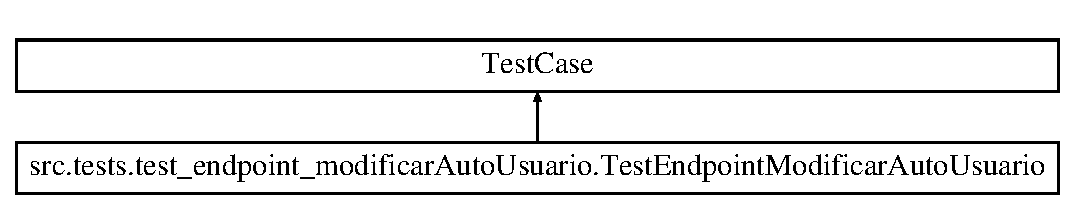
\includegraphics[height=2.000000cm]{classsrc_1_1tests_1_1test__endpoint__modificar_auto_usuario_1_1_test_endpoint_modificar_auto_usuario}
\end{center}
\end{figure}
\subsection*{Métodos públicos}
\begin{DoxyCompactItemize}
\item 
\hypertarget{classsrc_1_1tests_1_1test__endpoint__modificar_auto_usuario_1_1_test_endpoint_modificar_auto_usuario_a50e3f1030d58e5ee28c870d46302082f}{def {\bfseries set\-Up}}\label{classsrc_1_1tests_1_1test__endpoint__modificar_auto_usuario_1_1_test_endpoint_modificar_auto_usuario_a50e3f1030d58e5ee28c870d46302082f}

\item 
\hypertarget{classsrc_1_1tests_1_1test__endpoint__modificar_auto_usuario_1_1_test_endpoint_modificar_auto_usuario_a5ef67795fdc740779e272c717410debc}{def {\bfseries test\-\_\-camino\-\_\-feliz}}\label{classsrc_1_1tests_1_1test__endpoint__modificar_auto_usuario_1_1_test_endpoint_modificar_auto_usuario_a5ef67795fdc740779e272c717410debc}

\item 
\hypertarget{classsrc_1_1tests_1_1test__endpoint__modificar_auto_usuario_1_1_test_endpoint_modificar_auto_usuario_a0831ac6dd310647b3782ec23b7681c0c}{def {\bfseries test\-\_\-sin\-\_\-token}}\label{classsrc_1_1tests_1_1test__endpoint__modificar_auto_usuario_1_1_test_endpoint_modificar_auto_usuario_a0831ac6dd310647b3782ec23b7681c0c}

\item 
\hypertarget{classsrc_1_1tests_1_1test__endpoint__modificar_auto_usuario_1_1_test_endpoint_modificar_auto_usuario_a980a95f7e9d4d82ab24f0f31b1bbda91}{def {\bfseries test\-\_\-sin\-\_\-json}}\label{classsrc_1_1tests_1_1test__endpoint__modificar_auto_usuario_1_1_test_endpoint_modificar_auto_usuario_a980a95f7e9d4d82ab24f0f31b1bbda91}

\item 
\hypertarget{classsrc_1_1tests_1_1test__endpoint__modificar_auto_usuario_1_1_test_endpoint_modificar_auto_usuario_a9485c54519c28249990819d6ffdc3534}{def {\bfseries test\-\_\-token\-\_\-invalido}}\label{classsrc_1_1tests_1_1test__endpoint__modificar_auto_usuario_1_1_test_endpoint_modificar_auto_usuario_a9485c54519c28249990819d6ffdc3534}

\item 
\hypertarget{classsrc_1_1tests_1_1test__endpoint__modificar_auto_usuario_1_1_test_endpoint_modificar_auto_usuario_a78ac3e40946b8e76263b79d0efbebeaf}{def {\bfseries test\-\_\-conexion\-\_\-fallida}}\label{classsrc_1_1tests_1_1test__endpoint__modificar_auto_usuario_1_1_test_endpoint_modificar_auto_usuario_a78ac3e40946b8e76263b79d0efbebeaf}

\end{DoxyCompactItemize}
\subsection*{Atributos públicos}
\begin{DoxyCompactItemize}
\item 
\hypertarget{classsrc_1_1tests_1_1test__endpoint__modificar_auto_usuario_1_1_test_endpoint_modificar_auto_usuario_a159a7f74f65e2661eae3eb55347bd3b0}{{\bfseries app}}\label{classsrc_1_1tests_1_1test__endpoint__modificar_auto_usuario_1_1_test_endpoint_modificar_auto_usuario_a159a7f74f65e2661eae3eb55347bd3b0}

\end{DoxyCompactItemize}


La documentación para esta clase fue generada a partir del siguiente fichero\-:\begin{DoxyCompactItemize}
\item 
src/tests/test\-\_\-endpoint\-\_\-modificar\-Auto\-Usuario.\-py\end{DoxyCompactItemize}

\hypertarget{classsrc_1_1tests_1_1test__endpoint__obtener_posibles_viajes_1_1_test_endpoint_obtener_posibles_viajes}{\section{Referencia de la Clase src.\-tests.\-test\-\_\-endpoint\-\_\-obtener\-Posibles\-Viajes.\-Test\-Endpoint\-Obtener\-Posibles\-Viajes}
\label{classsrc_1_1tests_1_1test__endpoint__obtener_posibles_viajes_1_1_test_endpoint_obtener_posibles_viajes}\index{src.\-tests.\-test\-\_\-endpoint\-\_\-obtener\-Posibles\-Viajes.\-Test\-Endpoint\-Obtener\-Posibles\-Viajes@{src.\-tests.\-test\-\_\-endpoint\-\_\-obtener\-Posibles\-Viajes.\-Test\-Endpoint\-Obtener\-Posibles\-Viajes}}
}
Diagrama de herencias de src.\-tests.\-test\-\_\-endpoint\-\_\-obtener\-Posibles\-Viajes.\-Test\-Endpoint\-Obtener\-Posibles\-Viajes\begin{figure}[H]
\begin{center}
\leavevmode
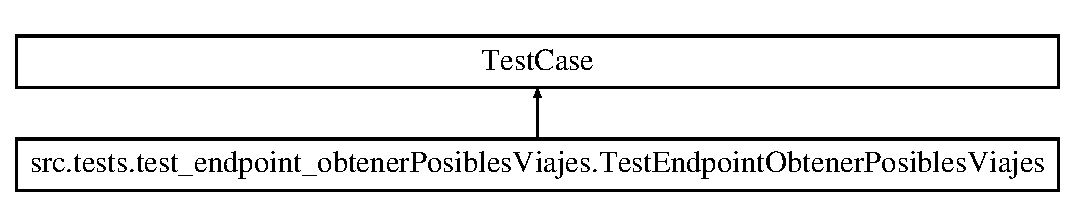
\includegraphics[height=2.000000cm]{classsrc_1_1tests_1_1test__endpoint__obtener_posibles_viajes_1_1_test_endpoint_obtener_posibles_viajes}
\end{center}
\end{figure}
\subsection*{Métodos públicos}
\begin{DoxyCompactItemize}
\item 
\hypertarget{classsrc_1_1tests_1_1test__endpoint__obtener_posibles_viajes_1_1_test_endpoint_obtener_posibles_viajes_a1ef195dcd5af6307b5ffa33913293ea4}{def {\bfseries set\-Up}}\label{classsrc_1_1tests_1_1test__endpoint__obtener_posibles_viajes_1_1_test_endpoint_obtener_posibles_viajes_a1ef195dcd5af6307b5ffa33913293ea4}

\item 
\hypertarget{classsrc_1_1tests_1_1test__endpoint__obtener_posibles_viajes_1_1_test_endpoint_obtener_posibles_viajes_a5d3d69246a3ec69783a4694a7d4c131b}{def {\bfseries test\-\_\-camino\-\_\-feliz}}\label{classsrc_1_1tests_1_1test__endpoint__obtener_posibles_viajes_1_1_test_endpoint_obtener_posibles_viajes_a5d3d69246a3ec69783a4694a7d4c131b}

\item 
\hypertarget{classsrc_1_1tests_1_1test__endpoint__obtener_posibles_viajes_1_1_test_endpoint_obtener_posibles_viajes_a61bd7cae163680abab4d28be9a6411e0}{def {\bfseries test\-\_\-token\-\_\-invalido}}\label{classsrc_1_1tests_1_1test__endpoint__obtener_posibles_viajes_1_1_test_endpoint_obtener_posibles_viajes_a61bd7cae163680abab4d28be9a6411e0}

\item 
\hypertarget{classsrc_1_1tests_1_1test__endpoint__obtener_posibles_viajes_1_1_test_endpoint_obtener_posibles_viajes_a7a9be52a8aec85a7178429e8e1650534}{def {\bfseries test\-\_\-conductor\-\_\-inexistente}}\label{classsrc_1_1tests_1_1test__endpoint__obtener_posibles_viajes_1_1_test_endpoint_obtener_posibles_viajes_a7a9be52a8aec85a7178429e8e1650534}

\end{DoxyCompactItemize}
\subsection*{Atributos públicos}
\begin{DoxyCompactItemize}
\item 
\hypertarget{classsrc_1_1tests_1_1test__endpoint__obtener_posibles_viajes_1_1_test_endpoint_obtener_posibles_viajes_a2b5c770e0a1cf3ecb36ad74f9bdc609a}{{\bfseries app}}\label{classsrc_1_1tests_1_1test__endpoint__obtener_posibles_viajes_1_1_test_endpoint_obtener_posibles_viajes_a2b5c770e0a1cf3ecb36ad74f9bdc609a}

\item 
\hypertarget{classsrc_1_1tests_1_1test__endpoint__obtener_posibles_viajes_1_1_test_endpoint_obtener_posibles_viajes_a861b60d20e96514d0c687c3dd36a09fd}{{\bfseries viajes\-Disponibles}}\label{classsrc_1_1tests_1_1test__endpoint__obtener_posibles_viajes_1_1_test_endpoint_obtener_posibles_viajes_a861b60d20e96514d0c687c3dd36a09fd}

\item 
\hypertarget{classsrc_1_1tests_1_1test__endpoint__obtener_posibles_viajes_1_1_test_endpoint_obtener_posibles_viajes_a289c0da43a33f59ed5440939bb62a850}{{\bfseries salida\-Correcta}}\label{classsrc_1_1tests_1_1test__endpoint__obtener_posibles_viajes_1_1_test_endpoint_obtener_posibles_viajes_a289c0da43a33f59ed5440939bb62a850}

\end{DoxyCompactItemize}


La documentación para esta clase fue generada a partir del siguiente fichero\-:\begin{DoxyCompactItemize}
\item 
src/tests/test\-\_\-endpoint\-\_\-obtener\-Posibles\-Viajes.\-py\end{DoxyCompactItemize}

\hypertarget{classsrc_1_1tests_1_1test__endpoint__token_1_1_test_endpoint_token}{\section{Referencia de la Clase src.\-tests.\-test\-\_\-endpoint\-\_\-token.\-Test\-Endpoint\-Token}
\label{classsrc_1_1tests_1_1test__endpoint__token_1_1_test_endpoint_token}\index{src.\-tests.\-test\-\_\-endpoint\-\_\-token.\-Test\-Endpoint\-Token@{src.\-tests.\-test\-\_\-endpoint\-\_\-token.\-Test\-Endpoint\-Token}}
}
Diagrama de herencias de src.\-tests.\-test\-\_\-endpoint\-\_\-token.\-Test\-Endpoint\-Token\begin{figure}[H]
\begin{center}
\leavevmode
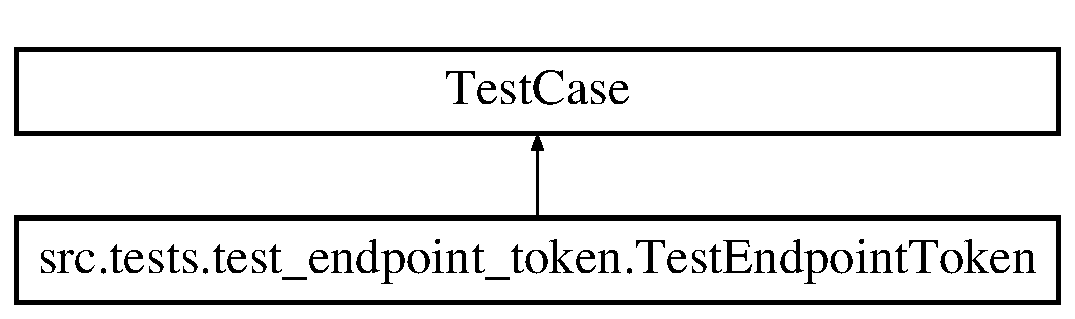
\includegraphics[height=2.000000cm]{classsrc_1_1tests_1_1test__endpoint__token_1_1_test_endpoint_token}
\end{center}
\end{figure}
\subsection*{Métodos públicos}
\begin{DoxyCompactItemize}
\item 
\hypertarget{classsrc_1_1tests_1_1test__endpoint__token_1_1_test_endpoint_token_a9ef8875211f02e65b52192ce2f508fc0}{def {\bfseries set\-Up}}\label{classsrc_1_1tests_1_1test__endpoint__token_1_1_test_endpoint_token_a9ef8875211f02e65b52192ce2f508fc0}

\item 
\hypertarget{classsrc_1_1tests_1_1test__endpoint__token_1_1_test_endpoint_token_aa96aa30f1ff08149cdf5cc1a5f104daf}{def {\bfseries test\-\_\-camino\-\_\-feliz}}\label{classsrc_1_1tests_1_1test__endpoint__token_1_1_test_endpoint_token_aa96aa30f1ff08149cdf5cc1a5f104daf}

\item 
\hypertarget{classsrc_1_1tests_1_1test__endpoint__token_1_1_test_endpoint_token_afd487d45efd20fc735502f562464427f}{def {\bfseries test\-\_\-sin\-\_\-json}}\label{classsrc_1_1tests_1_1test__endpoint__token_1_1_test_endpoint_token_afd487d45efd20fc735502f562464427f}

\item 
\hypertarget{classsrc_1_1tests_1_1test__endpoint__token_1_1_test_endpoint_token_afe3b5018948303f210740c1358081544}{def {\bfseries test\-\_\-fallo\-\_\-token}}\label{classsrc_1_1tests_1_1test__endpoint__token_1_1_test_endpoint_token_afe3b5018948303f210740c1358081544}

\item 
\hypertarget{classsrc_1_1tests_1_1test__endpoint__token_1_1_test_endpoint_token_ad0be9501a49f4781945844312d72f8ff}{def {\bfseries test\-\_\-no\-\_\-existe\-\_\-usuario}}\label{classsrc_1_1tests_1_1test__endpoint__token_1_1_test_endpoint_token_ad0be9501a49f4781945844312d72f8ff}

\item 
\hypertarget{classsrc_1_1tests_1_1test__endpoint__token_1_1_test_endpoint_token_a46767231478e601dd1136ad8bdd61637}{def {\bfseries test\-\_\-no\-\_\-se\-\_\-manda\-\_\-usuario}}\label{classsrc_1_1tests_1_1test__endpoint__token_1_1_test_endpoint_token_a46767231478e601dd1136ad8bdd61637}

\item 
\hypertarget{classsrc_1_1tests_1_1test__endpoint__token_1_1_test_endpoint_token_a2d4d7718c0586f39e1c4043b011619e6}{def {\bfseries test\-\_\-no\-\_\-se\-\_\-manda\-\_\-contrasena}}\label{classsrc_1_1tests_1_1test__endpoint__token_1_1_test_endpoint_token_a2d4d7718c0586f39e1c4043b011619e6}

\end{DoxyCompactItemize}
\subsection*{Atributos públicos}
\begin{DoxyCompactItemize}
\item 
\hypertarget{classsrc_1_1tests_1_1test__endpoint__token_1_1_test_endpoint_token_a35501d42c2a4197c00f7e3ccbf40ee64}{{\bfseries app}}\label{classsrc_1_1tests_1_1test__endpoint__token_1_1_test_endpoint_token_a35501d42c2a4197c00f7e3ccbf40ee64}

\end{DoxyCompactItemize}


La documentación para esta clase fue generada a partir del siguiente fichero\-:\begin{DoxyCompactItemize}
\item 
src/tests/test\-\_\-endpoint\-\_\-token.\-py\end{DoxyCompactItemize}

\hypertarget{classsrc_1_1tests_1_1test__token_1_1_test_token}{\section{Referencia de la Clase src.\-tests.\-test\-\_\-token.\-Test\-Token}
\label{classsrc_1_1tests_1_1test__token_1_1_test_token}\index{src.\-tests.\-test\-\_\-token.\-Test\-Token@{src.\-tests.\-test\-\_\-token.\-Test\-Token}}
}
Diagrama de herencias de src.\-tests.\-test\-\_\-token.\-Test\-Token\begin{figure}[H]
\begin{center}
\leavevmode
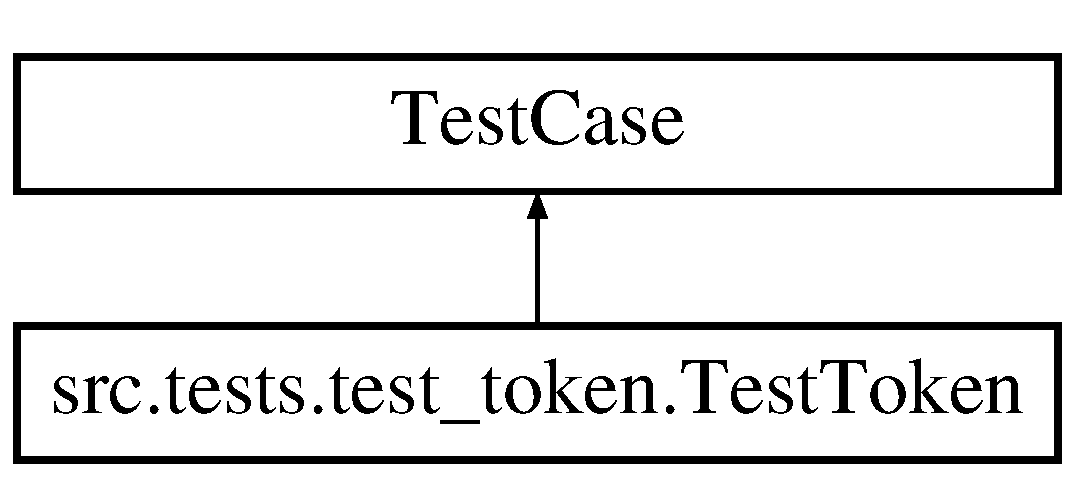
\includegraphics[height=2.000000cm]{classsrc_1_1tests_1_1test__token_1_1_test_token}
\end{center}
\end{figure}
\subsection*{Métodos públicos}
\begin{DoxyCompactItemize}
\item 
\hypertarget{classsrc_1_1tests_1_1test__token_1_1_test_token_a8aba7c3cd985db73a4308906cce602dc}{def {\bfseries test\-\_\-validar\-Token\-\_\-valido}}\label{classsrc_1_1tests_1_1test__token_1_1_test_token_a8aba7c3cd985db73a4308906cce602dc}

\item 
\hypertarget{classsrc_1_1tests_1_1test__token_1_1_test_token_a2422e590a46f5250a9b9cccbe827f9fa}{def {\bfseries test\-\_\-validar\-Token\-\_\-invalido}}\label{classsrc_1_1tests_1_1test__token_1_1_test_token_a2422e590a46f5250a9b9cccbe827f9fa}

\item 
\hypertarget{classsrc_1_1tests_1_1test__token_1_1_test_token_a87957ef104bfeba015dba8bfd7249cca}{def {\bfseries test\-\_\-obtener\-Token\-\_\-token\-Valido}}\label{classsrc_1_1tests_1_1test__token_1_1_test_token_a87957ef104bfeba015dba8bfd7249cca}

\item 
\hypertarget{classsrc_1_1tests_1_1test__token_1_1_test_token_a226ddb6f0540681775777a5b1520a0ac}{def {\bfseries test\-\_\-obtener\-Token\-\_\-token\-Expirado}}\label{classsrc_1_1tests_1_1test__token_1_1_test_token_a226ddb6f0540681775777a5b1520a0ac}

\item 
\hypertarget{classsrc_1_1tests_1_1test__token_1_1_test_token_afd81b1535b8cd821736efda5964b3c59}{def {\bfseries test\-\_\-obtener\-Token\-\_\-token\-Valido\-Datos\-Mal}}\label{classsrc_1_1tests_1_1test__token_1_1_test_token_afd81b1535b8cd821736efda5964b3c59}

\item 
\hypertarget{classsrc_1_1tests_1_1test__token_1_1_test_token_a9fdd70c5fd20ad1ab09d53377857991a}{def {\bfseries test\-\_\-obtener\-Token\-\_\-token\-Expirado\-Mal\-Encodeado}}\label{classsrc_1_1tests_1_1test__token_1_1_test_token_a9fdd70c5fd20ad1ab09d53377857991a}

\item 
\hypertarget{classsrc_1_1tests_1_1test__token_1_1_test_token_acc07ef6db3b245a9d4e0d33a5cb2ec46}{def {\bfseries test\-\_\-obtener\-Token\-\_\-token\-No\-Existente\-En\-Mongo}}\label{classsrc_1_1tests_1_1test__token_1_1_test_token_acc07ef6db3b245a9d4e0d33a5cb2ec46}

\item 
\hypertarget{classsrc_1_1tests_1_1test__token_1_1_test_token_a7e76dfd60722f62319508e396a1dbb94}{def {\bfseries test\-\_\-obtener\-Token\-\_\-token\-No\-Se\-Puede\-Recuperar\-De\-Mongo}}\label{classsrc_1_1tests_1_1test__token_1_1_test_token_a7e76dfd60722f62319508e396a1dbb94}

\item 
\hypertarget{classsrc_1_1tests_1_1test__token_1_1_test_token_af211afce1386a54cb9fde8c07c0036dc}{def {\bfseries test\-\_\-obtener\-Token\-\_\-token\-Driver\-No\-Se\-Puede\-Recuperar\-De\-Mongo}}\label{classsrc_1_1tests_1_1test__token_1_1_test_token_af211afce1386a54cb9fde8c07c0036dc}

\item 
\hypertarget{classsrc_1_1tests_1_1test__token_1_1_test_token_af2ba8ac11b6495774c4a0302fe3b86ad}{def {\bfseries test\-\_\-obtener\-Token\-\_\-token\-No\-Se\-Puede\-Almacenar\-De\-Mongo}}\label{classsrc_1_1tests_1_1test__token_1_1_test_token_af2ba8ac11b6495774c4a0302fe3b86ad}

\item 
\hypertarget{classsrc_1_1tests_1_1test__token_1_1_test_token_af2ba8ac11b6495774c4a0302fe3b86ad}{def {\bfseries test\-\_\-obtener\-Token\-\_\-token\-No\-Se\-Puede\-Almacenar\-De\-Mongo}}\label{classsrc_1_1tests_1_1test__token_1_1_test_token_af2ba8ac11b6495774c4a0302fe3b86ad}

\end{DoxyCompactItemize}


La documentación para esta clase fue generada a partir del siguiente fichero\-:\begin{DoxyCompactItemize}
\item 
src/tests/test\-\_\-token.\-py\end{DoxyCompactItemize}

\hypertarget{classsrc_1_1models_1_1token_1_1_token}{\section{Referencia de la Clase src.\-models.\-token.\-Token}
\label{classsrc_1_1models_1_1token_1_1_token}\index{src.\-models.\-token.\-Token@{src.\-models.\-token.\-Token}}
}


Clase para autenticacion y creacion del \hyperlink{classsrc_1_1models_1_1token_1_1_token}{Token}.  


Diagrama de herencias de src.\-models.\-token.\-Token\begin{figure}[H]
\begin{center}
\leavevmode
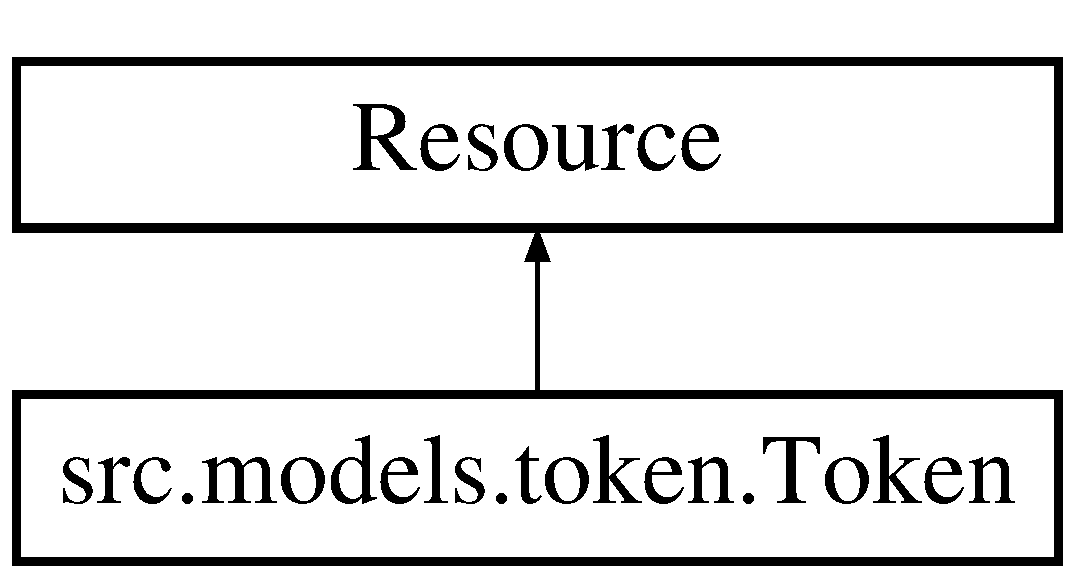
\includegraphics[height=2.000000cm]{classsrc_1_1models_1_1token_1_1_token}
\end{center}
\end{figure}
\subsection*{Métodos públicos}
\begin{DoxyCompactItemize}
\item 
\hypertarget{classsrc_1_1models_1_1token_1_1_token_a673568b00450f5644e8408eff2388cbe}{def {\bfseries \-\_\-\-\_\-init\-\_\-\-\_\-}}\label{classsrc_1_1models_1_1token_1_1_token_a673568b00450f5644e8408eff2388cbe}

\item 
def \hyperlink{classsrc_1_1models_1_1token_1_1_token_a6efab07d00f27b0a50478b27ba1fa920}{obtener\-Token}
\begin{DoxyCompactList}\small\item\em Autentica al usuario una unica vez. \end{DoxyCompactList}\item 
def \hyperlink{classsrc_1_1models_1_1token_1_1_token_aa38dc82b2a162d45ce1f4d492e8bf99c}{validar\-Token}
\begin{DoxyCompactList}\small\item\em Valida el token. \end{DoxyCompactList}\end{DoxyCompactItemize}
\subsection*{Atributos públicos}
\begin{DoxyCompactItemize}
\item 
\hypertarget{classsrc_1_1models_1_1token_1_1_token_af98d64a3e07c1a7104e801cf9ad40172}{{\bfseries C\-L\-A\-V\-E\-\_\-\-U\-L\-T\-R\-A\-S\-E\-C\-R\-E\-T\-A}}\label{classsrc_1_1models_1_1token_1_1_token_af98d64a3e07c1a7104e801cf9ad40172}

\end{DoxyCompactItemize}
\subsection*{Métodos privados}
\begin{DoxyCompactItemize}
\item 
\hypertarget{classsrc_1_1models_1_1token_1_1_token_a3ecc3ba1983a70ec195612df45d4ad3f}{def {\bfseries \-\_\-validar\-Token}}\label{classsrc_1_1models_1_1token_1_1_token_a3ecc3ba1983a70ec195612df45d4ad3f}

\item 
def \hyperlink{classsrc_1_1models_1_1token_1_1_token_a6dae16035576f9945a55ff47f09a56e7}{\-\_\-crear\-\_\-token}
\item 
def \hyperlink{classsrc_1_1models_1_1token_1_1_token_a2bd63e97694f42d32303c6d563d8c65e}{\-\_\-recuperar\-Token}
\begin{DoxyCompactList}\small\item\em Recupera el token de mongo\-D\-B. \end{DoxyCompactList}\item 
def \hyperlink{classsrc_1_1models_1_1token_1_1_token_a90daa7df2e19d41481bb3570a77de2f7}{\-\_\-generar\-Token}
\begin{DoxyCompactList}\small\item\em Genera y devuelve el token de autenticacion del usuario con el appserver. \end{DoxyCompactList}\item 
def \hyperlink{classsrc_1_1models_1_1token_1_1_token_a90eaf9eddea9e6f6b04c7a4b8542b71f}{\-\_\-almacenar\-Token}
\begin{DoxyCompactList}\small\item\em Guarda el token en mongo\-D\-B para accederlo de una. \end{DoxyCompactList}\item 
def \hyperlink{classsrc_1_1models_1_1token_1_1_token_a4f267817c4ea319c779cbbd77783c08d}{\-\_\-validar\-Token\-Login}
\begin{DoxyCompactList}\small\item\em Desempaqueta el token y valida los campos. \end{DoxyCompactList}\end{DoxyCompactItemize}


\subsection{Descripción detallada}
Clase para autenticacion y creacion del \hyperlink{classsrc_1_1models_1_1token_1_1_token}{Token}. 



\subsection{Documentación de las funciones miembro}
\hypertarget{classsrc_1_1models_1_1token_1_1_token_a90eaf9eddea9e6f6b04c7a4b8542b71f}{\index{src\-::models\-::token\-::\-Token@{src\-::models\-::token\-::\-Token}!\-\_\-almacenar\-Token@{\-\_\-almacenar\-Token}}
\index{\-\_\-almacenar\-Token@{\-\_\-almacenar\-Token}!src::models::token::Token@{src\-::models\-::token\-::\-Token}}
\subsubsection[{\-\_\-almacenar\-Token}]{\setlength{\rightskip}{0pt plus 5cm}def src.\-models.\-token.\-Token.\-\_\-almacenar\-Token (
\begin{DoxyParamCaption}
\item[{}]{self, }
\item[{}]{I\-D\-Usuario, }
\item[{}]{tipo\-Usuario, }
\item[{}]{nombre\-Usuario, }
\item[{}]{token}
\end{DoxyParamCaption}
)\hspace{0.3cm}{\ttfamily [private]}}}\label{classsrc_1_1models_1_1token_1_1_token_a90eaf9eddea9e6f6b04c7a4b8542b71f}


Guarda el token en mongo\-D\-B para accederlo de una. 

Devuelve true si se pudo guardar o false si no se pudo porque no existia el usuario


\begin{DoxyParams}{Parámetros}
{\em nombre\-Usuario} & Nombre del usuario. \\
\hline
{\em token} & token a guardar. \\
\hline
\end{DoxyParams}
\hypertarget{classsrc_1_1models_1_1token_1_1_token_a6dae16035576f9945a55ff47f09a56e7}{\index{src\-::models\-::token\-::\-Token@{src\-::models\-::token\-::\-Token}!\-\_\-crear\-\_\-token@{\-\_\-crear\-\_\-token}}
\index{\-\_\-crear\-\_\-token@{\-\_\-crear\-\_\-token}!src::models::token::Token@{src\-::models\-::token\-::\-Token}}
\subsubsection[{\-\_\-crear\-\_\-token}]{\setlength{\rightskip}{0pt plus 5cm}def src.\-models.\-token.\-Token.\-\_\-crear\-\_\-token (
\begin{DoxyParamCaption}
\item[{}]{self, }
\item[{}]{I\-D\-Usuario, }
\item[{}]{tipo\-Usuario, }
\item[{}]{nombre\-Usuario, }
\item[{}]{contrasena}
\end{DoxyParamCaption}
)\hspace{0.3cm}{\ttfamily [private]}}}\label{classsrc_1_1models_1_1token_1_1_token_a6dae16035576f9945a55ff47f09a56e7}
\begin{DoxyVerb}"Se crea un nuevo token.\end{DoxyVerb}
 \hypertarget{classsrc_1_1models_1_1token_1_1_token_a90daa7df2e19d41481bb3570a77de2f7}{\index{src\-::models\-::token\-::\-Token@{src\-::models\-::token\-::\-Token}!\-\_\-generar\-Token@{\-\_\-generar\-Token}}
\index{\-\_\-generar\-Token@{\-\_\-generar\-Token}!src::models::token::Token@{src\-::models\-::token\-::\-Token}}
\subsubsection[{\-\_\-generar\-Token}]{\setlength{\rightskip}{0pt plus 5cm}def src.\-models.\-token.\-Token.\-\_\-generar\-Token (
\begin{DoxyParamCaption}
\item[{}]{self, }
\item[{}]{nombre\-Usuario, }
\item[{}]{contrasena}
\end{DoxyParamCaption}
)\hspace{0.3cm}{\ttfamily [private]}}}\label{classsrc_1_1models_1_1token_1_1_token_a90daa7df2e19d41481bb3570a77de2f7}


Genera y devuelve el token de autenticacion del usuario con el appserver. 


\begin{DoxyParams}{Parámetros}
{\em nombre\-Usuario} & Nombre del usuario. \\
\hline
{\em contrasena} & Contrasena del usuario hasheada. \\
\hline
\end{DoxyParams}
\hypertarget{classsrc_1_1models_1_1token_1_1_token_a2bd63e97694f42d32303c6d563d8c65e}{\index{src\-::models\-::token\-::\-Token@{src\-::models\-::token\-::\-Token}!\-\_\-recuperar\-Token@{\-\_\-recuperar\-Token}}
\index{\-\_\-recuperar\-Token@{\-\_\-recuperar\-Token}!src::models::token::Token@{src\-::models\-::token\-::\-Token}}
\subsubsection[{\-\_\-recuperar\-Token}]{\setlength{\rightskip}{0pt plus 5cm}def src.\-models.\-token.\-Token.\-\_\-recuperar\-Token (
\begin{DoxyParamCaption}
\item[{}]{self, }
\item[{}]{nombre\-Usuario}
\end{DoxyParamCaption}
)\hspace{0.3cm}{\ttfamily [private]}}}\label{classsrc_1_1models_1_1token_1_1_token_a2bd63e97694f42d32303c6d563d8c65e}


Recupera el token de mongo\-D\-B. 

Devuelve el token o false.


\begin{DoxyParams}{Parámetros}
{\em nombre\-Usuario} & Nombre del usuario. \\
\hline
\end{DoxyParams}
\hypertarget{classsrc_1_1models_1_1token_1_1_token_a4f267817c4ea319c779cbbd77783c08d}{\index{src\-::models\-::token\-::\-Token@{src\-::models\-::token\-::\-Token}!\-\_\-validar\-Token\-Login@{\-\_\-validar\-Token\-Login}}
\index{\-\_\-validar\-Token\-Login@{\-\_\-validar\-Token\-Login}!src::models::token::Token@{src\-::models\-::token\-::\-Token}}
\subsubsection[{\-\_\-validar\-Token\-Login}]{\setlength{\rightskip}{0pt plus 5cm}def src.\-models.\-token.\-Token.\-\_\-validar\-Token\-Login (
\begin{DoxyParamCaption}
\item[{}]{self, }
\item[{}]{nombre\-Usuario, }
\item[{}]{contrasena, }
\item[{}]{token}
\end{DoxyParamCaption}
)\hspace{0.3cm}{\ttfamily [private]}}}\label{classsrc_1_1models_1_1token_1_1_token_a4f267817c4ea319c779cbbd77783c08d}


Desempaqueta el token y valida los campos. 

Devuelve true o false.


\begin{DoxyParams}{Parámetros}
{\em nombre\-Usuario} & Nombre del usuario. \\
\hline
{\em contrasena} & Contrasena del usuario hasheada. \\
\hline
{\em token} & token a validar. \\
\hline
\end{DoxyParams}
\hypertarget{classsrc_1_1models_1_1token_1_1_token_a6efab07d00f27b0a50478b27ba1fa920}{\index{src\-::models\-::token\-::\-Token@{src\-::models\-::token\-::\-Token}!obtener\-Token@{obtener\-Token}}
\index{obtener\-Token@{obtener\-Token}!src::models::token::Token@{src\-::models\-::token\-::\-Token}}
\subsubsection[{obtener\-Token}]{\setlength{\rightskip}{0pt plus 5cm}def src.\-models.\-token.\-Token.\-obtener\-Token (
\begin{DoxyParamCaption}
\item[{}]{self, }
\item[{}]{I\-D\-Usuario, }
\item[{}]{tipo\-Usuario, }
\item[{}]{nombre\-Usuario, }
\item[{}]{contrasena}
\end{DoxyParamCaption}
)}}\label{classsrc_1_1models_1_1token_1_1_token_a6efab07d00f27b0a50478b27ba1fa920}


Autentica al usuario una unica vez. 

Si el usuario no tenia un token anterior o expiro se crea uno y se almacena, sino se devuelve el que ya tenia asignado. \hypertarget{classsrc_1_1models_1_1token_1_1_token_aa38dc82b2a162d45ce1f4d492e8bf99c}{\index{src\-::models\-::token\-::\-Token@{src\-::models\-::token\-::\-Token}!validar\-Token@{validar\-Token}}
\index{validar\-Token@{validar\-Token}!src::models::token::Token@{src\-::models\-::token\-::\-Token}}
\subsubsection[{validar\-Token}]{\setlength{\rightskip}{0pt plus 5cm}def src.\-models.\-token.\-Token.\-validar\-Token (
\begin{DoxyParamCaption}
\item[{}]{self, }
\item[{}]{token}
\end{DoxyParamCaption}
)}}\label{classsrc_1_1models_1_1token_1_1_token_aa38dc82b2a162d45ce1f4d492e8bf99c}


Valida el token. 


\begin{DoxyParams}{Parámetros}
{\em token} & \hyperlink{classsrc_1_1models_1_1token_1_1_token}{Token} a validar. \\
\hline
\end{DoxyParams}


La documentación para esta clase fue generada a partir del siguiente fichero\-:\begin{DoxyCompactItemize}
\item 
src/models/token.\-py\end{DoxyCompactItemize}

\hypertarget{classsrc_1_1models_1_1user_1_1_user}{\section{Referencia de la Clase src.\-models.\-user.\-User}
\label{classsrc_1_1models_1_1user_1_1_user}\index{src.\-models.\-user.\-User@{src.\-models.\-user.\-User}}
}
Diagrama de herencias de src.\-models.\-user.\-User\begin{figure}[H]
\begin{center}
\leavevmode
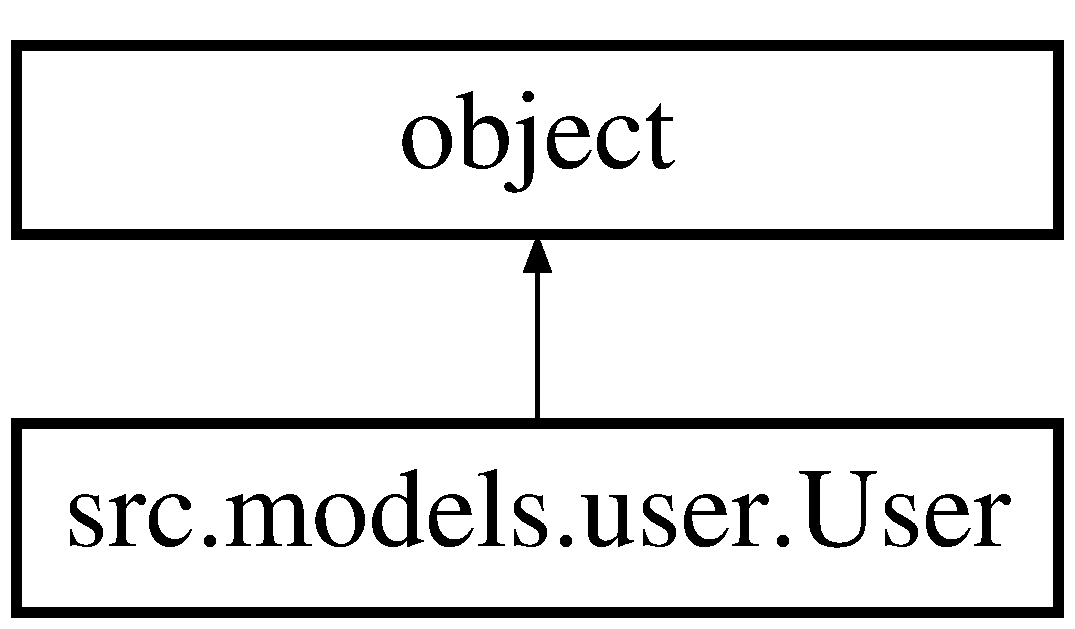
\includegraphics[height=2.000000cm]{classsrc_1_1models_1_1user_1_1_user}
\end{center}
\end{figure}
\subsection*{Métodos públicos}
\begin{DoxyCompactItemize}
\item 
\hypertarget{classsrc_1_1models_1_1user_1_1_user_a700cd275668883b1a33ba8748e2fa9b5}{def {\bfseries \-\_\-\-\_\-init\-\_\-\-\_\-}}\label{classsrc_1_1models_1_1user_1_1_user_a700cd275668883b1a33ba8748e2fa9b5}

\item 
\hypertarget{classsrc_1_1models_1_1user_1_1_user_a0017f93a5236a16c2e8cda903b287cf2}{def {\bfseries exists\-\_\-by\-\_\-username}}\label{classsrc_1_1models_1_1user_1_1_user_a0017f93a5236a16c2e8cda903b287cf2}

\item 
\hypertarget{classsrc_1_1models_1_1user_1_1_user_af6852baecb9f07aad7fa526b92d4fc03}{def {\bfseries exists\-\_\-by\-\_\-id}}\label{classsrc_1_1models_1_1user_1_1_user_af6852baecb9f07aad7fa526b92d4fc03}

\item 
\hypertarget{classsrc_1_1models_1_1user_1_1_user_ab86bb8e7b6e3b095773df938c80e2fbd}{def {\bfseries stored\-\_\-user\-\_\-in\-\_\-shared\-\_\-server}}\label{classsrc_1_1models_1_1user_1_1_user_ab86bb8e7b6e3b095773df938c80e2fbd}

\item 
\hypertarget{classsrc_1_1models_1_1user_1_1_user_a113d7cb1094a9fe8cf3756e6399a1a74}{def {\bfseries modify\-\_\-user\-\_\-in\-\_\-shared\-\_\-server}}\label{classsrc_1_1models_1_1user_1_1_user_a113d7cb1094a9fe8cf3756e6399a1a74}

\end{DoxyCompactItemize}
\subsection*{Atributos públicos}
\begin{DoxyCompactItemize}
\item 
\hypertarget{classsrc_1_1models_1_1user_1_1_user_a2a6520a054dbf86c2b8b95cc2bddd485}{{\bfseries user\-Id}}\label{classsrc_1_1models_1_1user_1_1_user_a2a6520a054dbf86c2b8b95cc2bddd485}

\item 
\hypertarget{classsrc_1_1models_1_1user_1_1_user_a8c48786e6e354ab921618a995b7a3644}{{\bfseries tipo}}\label{classsrc_1_1models_1_1user_1_1_user_a8c48786e6e354ab921618a995b7a3644}

\item 
\hypertarget{classsrc_1_1models_1_1user_1_1_user_a9f71617c28c98830fc5ab3c759cf7a1d}{{\bfseries usr}}\label{classsrc_1_1models_1_1user_1_1_user_a9f71617c28c98830fc5ab3c759cf7a1d}

\item 
\hypertarget{classsrc_1_1models_1_1user_1_1_user_ae94bf8f97ad07d3938e4f0f2839a0f45}{{\bfseries pwd}}\label{classsrc_1_1models_1_1user_1_1_user_ae94bf8f97ad07d3938e4f0f2839a0f45}

\item 
\hypertarget{classsrc_1_1models_1_1user_1_1_user_a0860e9aa254a148eb3cfefca4d495a9d}{{\bfseries fb}}\label{classsrc_1_1models_1_1user_1_1_user_a0860e9aa254a148eb3cfefca4d495a9d}

\item 
\hypertarget{classsrc_1_1models_1_1user_1_1_user_a891a862565bbc72c7f514c41e67ce692}{{\bfseries name}}\label{classsrc_1_1models_1_1user_1_1_user_a891a862565bbc72c7f514c41e67ce692}

\item 
\hypertarget{classsrc_1_1models_1_1user_1_1_user_a2681cfd922c69240eb6e27822a365b6a}{{\bfseries lastname}}\label{classsrc_1_1models_1_1user_1_1_user_a2681cfd922c69240eb6e27822a365b6a}

\item 
\hypertarget{classsrc_1_1models_1_1user_1_1_user_a32e1ec8137a307663b5041f97122031d}{{\bfseries email}}\label{classsrc_1_1models_1_1user_1_1_user_a32e1ec8137a307663b5041f97122031d}

\item 
\hypertarget{classsrc_1_1models_1_1user_1_1_user_a8c53cca4fcf93a9aae21f91de418b032}{{\bfseries birthdate}}\label{classsrc_1_1models_1_1user_1_1_user_a8c53cca4fcf93a9aae21f91de418b032}

\end{DoxyCompactItemize}


\subsection{Descripción detallada}
\begin{DoxyVerb}docstring for User\end{DoxyVerb}
 

La documentación para esta clase fue generada a partir del siguiente fichero\-:\begin{DoxyCompactItemize}
\item 
src/models/user.\-py\end{DoxyCompactItemize}

\hypertarget{classsrc_1_1resources_1_1user_control_1_1_user_controller}{\section{Referencia de la Clase src.\-resources.\-user\-Control.\-User\-Controller}
\label{classsrc_1_1resources_1_1user_control_1_1_user_controller}\index{src.\-resources.\-user\-Control.\-User\-Controller@{src.\-resources.\-user\-Control.\-User\-Controller}}
}


Clase para modificar, eliminar y obtener un usuario.  


Diagrama de herencias de src.\-resources.\-user\-Control.\-User\-Controller\begin{figure}[H]
\begin{center}
\leavevmode
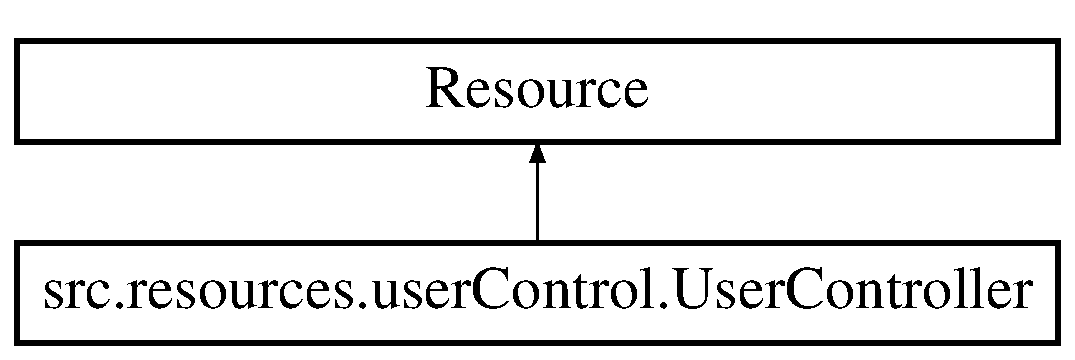
\includegraphics[height=2.000000cm]{classsrc_1_1resources_1_1user_control_1_1_user_controller}
\end{center}
\end{figure}
\subsection*{Métodos públicos}
\begin{DoxyCompactItemize}
\item 
\hypertarget{classsrc_1_1resources_1_1user_control_1_1_user_controller_af3100a3a699d047532e44bf0156af1c8}{def \hyperlink{classsrc_1_1resources_1_1user_control_1_1_user_controller_af3100a3a699d047532e44bf0156af1c8}{put}}\label{classsrc_1_1resources_1_1user_control_1_1_user_controller_af3100a3a699d047532e44bf0156af1c8}

\begin{DoxyCompactList}\small\item\em Put\-: modifica un usuario. \end{DoxyCompactList}\item 
\hypertarget{classsrc_1_1resources_1_1user_control_1_1_user_controller_afc4fd14e1b864baf878d7a731abb75ab}{def \hyperlink{classsrc_1_1resources_1_1user_control_1_1_user_controller_afc4fd14e1b864baf878d7a731abb75ab}{get}}\label{classsrc_1_1resources_1_1user_control_1_1_user_controller_afc4fd14e1b864baf878d7a731abb75ab}

\begin{DoxyCompactList}\small\item\em Get\-: obtiene info de un usuario. \end{DoxyCompactList}\item 
\hypertarget{classsrc_1_1resources_1_1user_control_1_1_user_controller_ac47a7ebe7f6e2791222681665cd7d021}{def \hyperlink{classsrc_1_1resources_1_1user_control_1_1_user_controller_ac47a7ebe7f6e2791222681665cd7d021}{delete}}\label{classsrc_1_1resources_1_1user_control_1_1_user_controller_ac47a7ebe7f6e2791222681665cd7d021}

\begin{DoxyCompactList}\small\item\em Delete\-: elimina un usuario. \end{DoxyCompactList}\end{DoxyCompactItemize}


\subsection{Descripción detallada}
Clase para modificar, eliminar y obtener un usuario. 

La documentación para esta clase fue generada a partir del siguiente fichero\-:\begin{DoxyCompactItemize}
\item 
src/resources/user\-Control.\-py\end{DoxyCompactItemize}

\hypertarget{classsrc_1_1resources_1_1usuario_modificar_posicion_1_1_usuario_modificar_posicion}{\section{Referencia de la Clase src.\-resources.\-usuario\-Modificar\-Posicion.\-Usuario\-Modificar\-Posicion}
\label{classsrc_1_1resources_1_1usuario_modificar_posicion_1_1_usuario_modificar_posicion}\index{src.\-resources.\-usuario\-Modificar\-Posicion.\-Usuario\-Modificar\-Posicion@{src.\-resources.\-usuario\-Modificar\-Posicion.\-Usuario\-Modificar\-Posicion}}
}


Clase para actualizar la posicion de un usuario.  


Diagrama de herencias de src.\-resources.\-usuario\-Modificar\-Posicion.\-Usuario\-Modificar\-Posicion\begin{figure}[H]
\begin{center}
\leavevmode
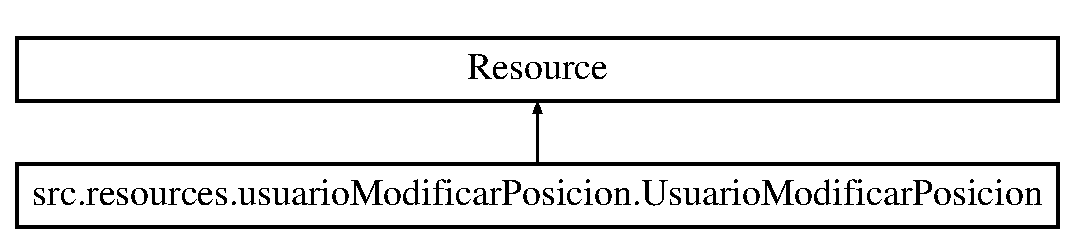
\includegraphics[height=2.000000cm]{classsrc_1_1resources_1_1usuario_modificar_posicion_1_1_usuario_modificar_posicion}
\end{center}
\end{figure}
\subsection*{Métodos públicos}
\begin{DoxyCompactItemize}
\item 
\hypertarget{classsrc_1_1resources_1_1usuario_modificar_posicion_1_1_usuario_modificar_posicion_a3510528dc54022281dbc9a5756507bec}{def {\bfseries \-\_\-\-\_\-init\-\_\-\-\_\-}}\label{classsrc_1_1resources_1_1usuario_modificar_posicion_1_1_usuario_modificar_posicion_a3510528dc54022281dbc9a5756507bec}

\item 
def \hyperlink{classsrc_1_1resources_1_1usuario_modificar_posicion_1_1_usuario_modificar_posicion_aa836c3ed2ae1d5124b5f093b99c789d0}{put}
\begin{DoxyCompactList}\small\item\em Actualiza los datos de posicion de un usuario. \end{DoxyCompactList}\end{DoxyCompactItemize}
\subsection*{Atributos públicos}
\begin{DoxyCompactItemize}
\item 
\hypertarget{classsrc_1_1resources_1_1usuario_modificar_posicion_1_1_usuario_modificar_posicion_a45af22de264a650894690011ae1a1489}{{\bfseries autenticador}}\label{classsrc_1_1resources_1_1usuario_modificar_posicion_1_1_usuario_modificar_posicion_a45af22de264a650894690011ae1a1489}

\end{DoxyCompactItemize}
\subsection*{Métodos privados}
\begin{DoxyCompactItemize}
\item 
def \hyperlink{classsrc_1_1resources_1_1usuario_modificar_posicion_1_1_usuario_modificar_posicion_aae13c7944d856a343f6125fd2e4421c4}{\-\_\-get\-\_\-data\-\_\-from\-\_\-request}
\begin{DoxyCompactList}\small\item\em Obtiene la propiedad del json contenido de la request. \end{DoxyCompactList}\item 
def \hyperlink{classsrc_1_1resources_1_1usuario_modificar_posicion_1_1_usuario_modificar_posicion_a54d77c4941b97883c98d55b1cddc5930}{\-\_\-validate\-\_\-request}
\begin{DoxyCompactList}\small\item\em Valida que haya una request completa. \end{DoxyCompactList}\item 
def \hyperlink{classsrc_1_1resources_1_1usuario_modificar_posicion_1_1_usuario_modificar_posicion_a4e9232f8e1f36581c5bac7a79c825f76}{\-\_\-validar\-\_\-token}
\begin{DoxyCompactList}\small\item\em Valida al usuario. \end{DoxyCompactList}\item 
def \hyperlink{classsrc_1_1resources_1_1usuario_modificar_posicion_1_1_usuario_modificar_posicion_ae6aa1e259bed2ae4e47f89c3ee86a28d}{\-\_\-actualizar\-\_\-posicion\-\_\-usuario}
\end{DoxyCompactItemize}


\subsection{Descripción detallada}
Clase para actualizar la posicion de un usuario. 



\subsection{Documentación de las funciones miembro}
\hypertarget{classsrc_1_1resources_1_1usuario_modificar_posicion_1_1_usuario_modificar_posicion_ae6aa1e259bed2ae4e47f89c3ee86a28d}{\index{src\-::resources\-::usuario\-Modificar\-Posicion\-::\-Usuario\-Modificar\-Posicion@{src\-::resources\-::usuario\-Modificar\-Posicion\-::\-Usuario\-Modificar\-Posicion}!\-\_\-actualizar\-\_\-posicion\-\_\-usuario@{\-\_\-actualizar\-\_\-posicion\-\_\-usuario}}
\index{\-\_\-actualizar\-\_\-posicion\-\_\-usuario@{\-\_\-actualizar\-\_\-posicion\-\_\-usuario}!src::resources::usuarioModificarPosicion::UsuarioModificarPosicion@{src\-::resources\-::usuario\-Modificar\-Posicion\-::\-Usuario\-Modificar\-Posicion}}
\subsubsection[{\-\_\-actualizar\-\_\-posicion\-\_\-usuario}]{\setlength{\rightskip}{0pt plus 5cm}def src.\-resources.\-usuario\-Modificar\-Posicion.\-Usuario\-Modificar\-Posicion.\-\_\-actualizar\-\_\-posicion\-\_\-usuario (
\begin{DoxyParamCaption}
\item[{}]{self, }
\item[{}]{I\-D\-Usuario, }
\item[{}]{x, }
\item[{}]{y}
\end{DoxyParamCaption}
)\hspace{0.3cm}{\ttfamily [private]}}}\label{classsrc_1_1resources_1_1usuario_modificar_posicion_1_1_usuario_modificar_posicion_ae6aa1e259bed2ae4e47f89c3ee86a28d}
\begin{DoxyVerb}Convierte a metros\end{DoxyVerb}
 \hypertarget{classsrc_1_1resources_1_1usuario_modificar_posicion_1_1_usuario_modificar_posicion_aae13c7944d856a343f6125fd2e4421c4}{\index{src\-::resources\-::usuario\-Modificar\-Posicion\-::\-Usuario\-Modificar\-Posicion@{src\-::resources\-::usuario\-Modificar\-Posicion\-::\-Usuario\-Modificar\-Posicion}!\-\_\-get\-\_\-data\-\_\-from\-\_\-request@{\-\_\-get\-\_\-data\-\_\-from\-\_\-request}}
\index{\-\_\-get\-\_\-data\-\_\-from\-\_\-request@{\-\_\-get\-\_\-data\-\_\-from\-\_\-request}!src::resources::usuarioModificarPosicion::UsuarioModificarPosicion@{src\-::resources\-::usuario\-Modificar\-Posicion\-::\-Usuario\-Modificar\-Posicion}}
\subsubsection[{\-\_\-get\-\_\-data\-\_\-from\-\_\-request}]{\setlength{\rightskip}{0pt plus 5cm}def src.\-resources.\-usuario\-Modificar\-Posicion.\-Usuario\-Modificar\-Posicion.\-\_\-get\-\_\-data\-\_\-from\-\_\-request (
\begin{DoxyParamCaption}
\item[{}]{self, }
\item[{}]{nombre\-Propiedad}
\end{DoxyParamCaption}
)\hspace{0.3cm}{\ttfamily [private]}}}\label{classsrc_1_1resources_1_1usuario_modificar_posicion_1_1_usuario_modificar_posicion_aae13c7944d856a343f6125fd2e4421c4}


Obtiene la propiedad del json contenido de la request. 

\hypertarget{classsrc_1_1resources_1_1usuario_modificar_posicion_1_1_usuario_modificar_posicion_a4e9232f8e1f36581c5bac7a79c825f76}{\index{src\-::resources\-::usuario\-Modificar\-Posicion\-::\-Usuario\-Modificar\-Posicion@{src\-::resources\-::usuario\-Modificar\-Posicion\-::\-Usuario\-Modificar\-Posicion}!\-\_\-validar\-\_\-token@{\-\_\-validar\-\_\-token}}
\index{\-\_\-validar\-\_\-token@{\-\_\-validar\-\_\-token}!src::resources::usuarioModificarPosicion::UsuarioModificarPosicion@{src\-::resources\-::usuario\-Modificar\-Posicion\-::\-Usuario\-Modificar\-Posicion}}
\subsubsection[{\-\_\-validar\-\_\-token}]{\setlength{\rightskip}{0pt plus 5cm}def src.\-resources.\-usuario\-Modificar\-Posicion.\-Usuario\-Modificar\-Posicion.\-\_\-validar\-\_\-token (
\begin{DoxyParamCaption}
\item[{}]{self}
\end{DoxyParamCaption}
)\hspace{0.3cm}{\ttfamily [private]}}}\label{classsrc_1_1resources_1_1usuario_modificar_posicion_1_1_usuario_modificar_posicion_a4e9232f8e1f36581c5bac7a79c825f76}


Valida al usuario. 

\hypertarget{classsrc_1_1resources_1_1usuario_modificar_posicion_1_1_usuario_modificar_posicion_a54d77c4941b97883c98d55b1cddc5930}{\index{src\-::resources\-::usuario\-Modificar\-Posicion\-::\-Usuario\-Modificar\-Posicion@{src\-::resources\-::usuario\-Modificar\-Posicion\-::\-Usuario\-Modificar\-Posicion}!\-\_\-validate\-\_\-request@{\-\_\-validate\-\_\-request}}
\index{\-\_\-validate\-\_\-request@{\-\_\-validate\-\_\-request}!src::resources::usuarioModificarPosicion::UsuarioModificarPosicion@{src\-::resources\-::usuario\-Modificar\-Posicion\-::\-Usuario\-Modificar\-Posicion}}
\subsubsection[{\-\_\-validate\-\_\-request}]{\setlength{\rightskip}{0pt plus 5cm}def src.\-resources.\-usuario\-Modificar\-Posicion.\-Usuario\-Modificar\-Posicion.\-\_\-validate\-\_\-request (
\begin{DoxyParamCaption}
\item[{}]{self}
\end{DoxyParamCaption}
)\hspace{0.3cm}{\ttfamily [private]}}}\label{classsrc_1_1resources_1_1usuario_modificar_posicion_1_1_usuario_modificar_posicion_a54d77c4941b97883c98d55b1cddc5930}


Valida que haya una request completa. 

\hypertarget{classsrc_1_1resources_1_1usuario_modificar_posicion_1_1_usuario_modificar_posicion_aa836c3ed2ae1d5124b5f093b99c789d0}{\index{src\-::resources\-::usuario\-Modificar\-Posicion\-::\-Usuario\-Modificar\-Posicion@{src\-::resources\-::usuario\-Modificar\-Posicion\-::\-Usuario\-Modificar\-Posicion}!put@{put}}
\index{put@{put}!src::resources::usuarioModificarPosicion::UsuarioModificarPosicion@{src\-::resources\-::usuario\-Modificar\-Posicion\-::\-Usuario\-Modificar\-Posicion}}
\subsubsection[{put}]{\setlength{\rightskip}{0pt plus 5cm}def src.\-resources.\-usuario\-Modificar\-Posicion.\-Usuario\-Modificar\-Posicion.\-put (
\begin{DoxyParamCaption}
\item[{}]{self, }
\item[{}]{I\-D\-Usuario}
\end{DoxyParamCaption}
)}}\label{classsrc_1_1resources_1_1usuario_modificar_posicion_1_1_usuario_modificar_posicion_aa836c3ed2ae1d5124b5f093b99c789d0}


Actualiza los datos de posicion de un usuario. 



La documentación para esta clase fue generada a partir del siguiente fichero\-:\begin{DoxyCompactItemize}
\item 
src/resources/usuario\-Modificar\-Posicion.\-py\end{DoxyCompactItemize}

%--- End generated contents ---

% Index
\newpage
\phantomsection
\addcontentsline{toc}{chapter}{Índice}
\printindex

\end{document}
